 \documentclass[review]{elsarticle}
\usepackage[utf8]{inputenc}
\providecommand{\tightlist}{%
  \setlength{\itemsep}{0pt}\setlength{\parskip}{0pt}}
\textwidth 6.75in
\oddsidemargin -0.15in
\evensidemargin -0.15in
\textheight 9in
\topmargin -0.5in
\usepackage{hyperref}%lineno,
%\modulolinenumbers[1]
\usepackage{amssymb,amsmath}
\renewcommand*{\appendixname}{}
%\include{../bootstrap/initial/software/Latex}
%\journal{Fisheries research}

%%%%%%%%%%%%%%%%%%%%%%%
%% Elsevier bibliography styles
%%%%%%%%%%%%%%%%%%%%%%%
%% To change the style, put a % in front of the second line of the current style and
%% remove the % from the second line of the style you would like to use.
%%%%%%%%%%%%%%%%%%%%%%%

%% Numbered
%\bibliographystyle{model1-num-names}

%% Numbered without titles
%\bibliographystyle{model1a-num-names}

%% Harvard
\bibliographystyle{model2-names.bst}\biboptions{authoryear}

%% Vancouver numbered
%\usepackage{numcompress}\bibliographystyle{model3-num-names}

%% Vancouver name/year
%\usepackage{numcompress}\bibliographystyle{model4-names}\biboptions{authoryear}

%% APA style
%\bibliographystyle{model5-names}\biboptions{authoryear}

%% AMA style
%\usepackage{numcompress}\bibliographystyle{model6-num-names}

%% `Elsevier LaTeX' style
%\bibliographystyle{natbib}
%%%%%%%%%%%%%%%%%%%%%%%

\usepackage{Sweave}
\begin{document}
\Sconcordance{concordance:Assessment2023prov_May8.tex:Assessment2023prov_May8.Rnw:%
1 48 1 1 0 185 1 1 1219 730 1 1 54 432 1 1 68 616 1}


\begin{frontmatter}

\title{Gadget for anchovy 9a South: Model description and results to provide catch advice and reference points (WGHANSA-1 2023)}
%%\tnotetext[mytitlenote]{Fully documented templates are available in the elsarticle package on \href{http://www.ctan.org/tex-archive/macros/latex/contrib/elsarticle}{CTAN}.}

%% Group authors per affiliation:
\author[a]{Margarita Mar{\'i}a Rinc{\'o}n\corref{cor1}}
\ead{margarita.rincon@ieo.csic.es}
%\address[a]{Department of Coastal Ecology and Management, Instituto de Ciencias Marinas de Andaluc{\'i}a, Consejo Superior de Investigaciones Cient{\'i}ficas, Avda Rep{\'u}blica Saharaui 2, 11519 Puerto Real, C{\'a}diz, Spain}
\address[a]{Instituto Español de Oceanograf{\'i}a (IEO-CSIC), Centro Oceanográfico de Cádiz, Puerto
pesquero, Muelle de Levante s/n, Apdo. 2609, 11006 Cádiz, Spain}
 \cortext[cor1]{Corresponding author}
 

\author[a]{Fernando Ramos}

\author[a]{Jorge Tornero}  

\author[b]{Susana Garrido}

\address[b]{Instituto Portugues do Mar e da Atmosfera-IPMA, Av. Brasília, 6, 1449-006 Lisboa, Portugal}

\author[c]{Bjarki Elvarsson}

\address[c]{Marine and Freshwater Research Institute, Fornubúdum 5
220 Hafnarfjördur, Iceland}

\author[c]{Jamie Lentin}

%\address[d]{Shuttlethread}

%\begin{abstract}
%This template helps you to create a properly formatted \LaTeX\ manuscript.
%\end{abstract}

%\begin{keyword}
%\texttt{elsarticle.cls}\sep \LaTeX\sep Elsevier \sep template
%\MSC[2010] 00-01\sep  99-00
%\end{keyword}

\end{frontmatter}

%\linenumbers

\section{Background}

The model specifications presented below correspond to those benchmarked in WKPELA 2018. The main difference is that results are presented now for the end of the second quarter of each year instead of be presented at the end of the fourth quarter. This responds to practical modifications in the definition of the assessment year, now it goes from July 1st to June 30th of the next year. Specific model assumptions for this year are presented in section \ref{obser} and \ref{Remark}, as well as estimated parameters after optimization in Table \ref{Symbols}.


\section{Model Description}




%A Gadget model works making forward simulations and minimizing an objective (negative weighted log-likelihood) function that measures the difference between the model and data, the discrepancy is presented as a likelihood score for each time period and model component. Gadget structure and options are described in \citet{begley_overview_2004}.



%ThereAs mentioned before last years represent a stable period for the fishery in terms of anthropogenic and environmental forces. 
 %There is a change in catches selectivity pattern in year 2001sFrom catches length distribution time series selectivity pattern changes.
 
 
 Gadget is an age-length-structured model that integrates different sources of information in order to produce a diagnose of the stock dynamics.  It works making forward simulations and minimizing an objective (negative log-likelihood) function that measures the difference between the model and data, the discrepancy is presented as a likelihood score for each time period and model component.% Gadget structure and options are described in \citet{begley_overview_2004}.
 
 
 
 % that implements forward simulations while minimizing an objective function (negative log-likelihood) that measures the difference between the model and data. Discrepancies between model and data are presented as a likelihood score for each time period and model component. %Gadget structure and options are described in detail at \citet{begley_overview_2004}.

 
 The general Gadget model description and all the options available can be found in Gadget manual \citep{begley_gadget_2004} and some specific examples can be found in \citet{taylor_simple_2007}, \citet{elvarsson_bootstrap_2014} and WKICEMSE assessment for Ling (Elvarsson, 2017).  The latest was used as a guide for this document.
 
 The Gadget model implementation consists in three parts, a simulation of biological dynamics of the population (simulation model), a fitting of the model to observed data using a weighted log-likelihood function (observation model) and the optimization of the parameters using different iterative algorithms.   

%The simple models chosen are part of a summary of data-limited methods described in \textbf{DLMtool manual} and there is an interactive way to use them available at \url{http://www.datalimitedtoolkit.org/}

A list of the symbols used and estimated parameters is presented in  Table \ref{Symbols} and a graph with the Gadget model structure presented in the last benchmark (WKPELA 2018) is available at \href{http://prezi.com/j8rinhq5kstg/?utm_campaign=share&utm_medium=copy}{Gadget structure graph}.





 
 % Gadget is a tool that integrates different sources of information in order to produce a diagnose of the stock dynamics. Gadget is an age-length-structured model that implements forward simulations while minimizing an objective function (negative log-likelihood) that measures the difference between the model and data. Discrepancies between model and data are presented as a likelihood score for each time period and model component. Gadget structure and options are described in detail at \citet{begley_overview_2004}.




 
 





 
 
 
 
%  \begin{equation}
% \label{eq:inlen}
% \Delta l =(l_\infty - l)(1-e^{k\Delta t}),
% \end{equation}
% 
% where $\Delta t$ is the length of the timestep, $l_\infty$ is the terminal length and $k$ is the growth rate parameter.
% 
% The corresponding increase in weight of the stock is given by:
% 
% \begin{equation}
% \label{eq:inwei}
% \Delta w=a ((l + \Delta l)^b - l^b),
% \end{equation}

% \subsection{Simulation model}
% %\end{itemize}
% 
% The model consists of one stock component of anchovy (\textit{Engraulis encrasicolus}) in the ICES subdivision, IX.a South-Atlantic Iberian waters, Gulf of Cádiz. Gadget works by keeping track of the number of individuals, $N_{a,l,y,t},$ at ages $a = 0, \dots,3$, at lengths $l = 3,3.5,4,4.5, \dots,22$, at years $y=1989,\dots,2015$, and each year divided into quarters $t =1, \dots, 4.$. The last time step of a year involves increasing the age by one year, except for the last age group, which its age remains unchanged and the age group next to is added to it, like a 'plus group' including all ages from the oldest age onwards \citep{taylor_simple_2007}.



% specific region defined by $ r $ = IXa (Division 9.a South-Atlantic Iberian waters, Gulf of Cádiz). Gadget works by keeping track of the number of individual and mean weight at age $ a$ = 0.3, at reference weight  , at length $l$ = 3.22 with a step size$ dl $= 0.5 between each length group, with a specified timestep$ t $= 4 for each year ($y$) from 1988 to 2015. The length of the timestep is denoted by $\Delta t$.

% \subsubsection*{Growth}
%  
%  
% Growth in terms of length and weight were formulated as $\Delta l =(l_\infty - l)(1-e^{k\Delta t})$ and $\Delta w=a ((l + \Delta l)^b - l^b)$, respectively, where $\Delta t$ is the length of the timestep, $l_\infty$ assumed as fixed and equal to 19 $cm$ is the terminal length and $k$ is the growth rate parameter. Parameters  $l_{\infty}, a=2.9e^{-5}$ and $b=3.3438,$ were obtained for this stock by \citep{millan_reproductive_1999}. Natural mortality at age, $M_{0}=1.17$ and $M_{1}=0.43,$ was derived from anchovy mortality in the Alboran Sea \textbf{GFCM2009}. The values for $M_{2}$ and $M_{3}$ were chosen high enough to be consistent with catches at age data, where individuals older than two years are rarely found. Gadget integrates data and processes to produce a quarterly diagnose of recruits which is added to the smallest age group each quarter. Size restrictions to the fishery were incepted in 2000. As a consequence, selectivity paramenters are divided into two periods: 1998-2000 and 2001-2015.

% Likelihood files were prepared for Gadget format using the \textit{mfdb} R package and, weighting of likelihood components and forecasting procedures were implemented in R with the gadget.iterative and gadget.forward function, respectively, from \textit{Rgadget} package. The gadget.iterative function follows the approach presented in \citet{taylor_simple_2007},  based on the iterative reweighting scheme of \citet{stefansson_comparing_1998,stefansson_issues_2003}. %It compares the results from a gadget run using the inverse 
% This method runs Gadget several times to get a likelihood score of each likelihood component, in each iteration the weigth of a dataset is greatly increased while the others remain constant and equal to one.  The gadget.forward function performs a Gadget simulation, using the parameter values found after optimization. It was necessary to modify the original function to include different recruitment assumptions.

% Weighting of likelihood components were done following the approach presented in \citet{taylor_simple_2007} and in the apppendix of \citet{elvarsson_bootstrap_2014} based on the iterative reweighting scheme of \citet{stefansson_comparing_1998} and \citet{stefansson_issues_2003}. %It compares the results from a gadget run using the inverse 
%Forecasting was implemented  by using the parameter values found after minimizing the objective weighted function and assuming a constant effort equal to 0.85.% (negative weighted log-likelihood) function (negative weighted log-likelihood) function an optimization run 


%in each iteration one dataset weight is greatly increased while the others remain constant and equal to one. 

% Forecasting were implemented performing a Gadget simulation, using the parameter values found after optimization, while
% weighting of likelihood components were done following the approach presented in \citet{taylor_simple_2007},  based on the iterative reweighting scheme of \citet{stefansson_comparing_1998,stefansson_issues_2003}. %It compares the results from a gadget run using the inverse 
% This method runs Gadget several times to get a likelihood score of each likelihood component, in each iteration the weigth of a dataset is greatly increased while the others remain constant and equal to one. 

% Input data, weighting and forecasting processes were implemented in R using the \textit{mfdb} R package and, gadget.iterative and gadget.forward function from \textit{Rgadget} package, respectively. Further details of model implementation and weighting of likelihood components are presented below



% \subsubsection{Data}
% 
% The following information was extracted from ICES reports (public) and from IEO datasets (non public).  The following datasets are used in Gadget for likelihood components. Gadget classify this information as different types of components, time period and component are specified  in parenthesis:
% \begin{itemize}
%  \item Length distribution of landings (1998-2015, catchdistribution)
% \item Age distribution of landings (1998-2015, catchdistribution)
% \item Landings mean length at age of landings(1988-2015, catchstatistics)
% \item Biomass survey indexes from ECOCADIZ survey. (Second quarter 2004, 2006; third quarter 2007, 2009, 2010, 2013 and 2014, surveyindexes)
% \item Age and length distribution of survey ECOCADIZ (Second quarter 2004, 2006; third quarter 2007, 2009, 2010, 2013 and 2014, catchdistribution)
% \item Biomass survey indexes from PELAGO survey. (First quarter 1999, 2001-2003, second quarter 2005-2010, 2014, surveyindexes)
% \item Age and length distribution of survey PELAGO (First quarter 1999, 2001-2003, second quarter 2005-2010, 2014, catchdistribution)
% \item Biomass survey indexes from SAR survey. (Last quarter 1998, 2000,2001, 2007 and 2012, surveyindexes)
% \end{itemize}
% 
% Quaterly catches in numbers are used for the fleet information, which is assumed by Gadget as a predator.


% \subsubsection{Assumptions}
% \begin{itemize}
% \item Some parameter values as $L_{\infty}=19$ and $a=2.9e^{-5}, b=3.3438,$ were extracted from data of the Gulf of Cádiz sistematically sampled during 4 years \citep{millan_reproductive_1999}. They were assumed fixed in the following equations accounting for growth in terms of length and weight, respectively:  
% $L(t)=L_{\infty}(1-\exp^{tK})$ and $W(t)=aL(t)^b.$
% 
% \item Natural mortality at age was also considered fixed with $M_{0}=1.17$ and $M_{1}=0.43,$ using data from anchovy mortality in Alboran Sea \citep{GFCM2009}. The values for $M_{2}$ and $M_{3}$ were chosen higher enough to be coherent with catches at age data, where there is rarely to find individuals older than two years.  
% 
% \item A number (calculated by the model) of individuals considered as recruits, is added once each year to the smallest age group each quarter.
% 
% \item There was a size restriction from 1995, that were only effective until 2001. As a consequence it was neccesary to define different parameters for two different selectivity patterns. One from 1988 to 2000, and the other from 2001 to 2015. 
% 
% \end{itemize}
% 
% 
% \subsubsection{Implementation and weighting procedure}
% 
% Likelihood files were prepared for Gadget format using the \textit{mfdb} R package and, running and weighting procedures were implemented in R with the gadget.iterative function from \textit{Rgadget} package. This function follows the approach presented in \citet{taylor_simple_2007},  based on the iterative reweighting scheme of \citet{stefansson_comparing_1998,stefansson_issues_2003}. %It compares the results from a gadget run using the inverse 
% This method runs Gadget several times to get a likelihood score of each likelihood component, in each iteration the weigth of a dataset is greatly increased while the others remain constant and equal to one.



 

\begin{table}[h]

\centering

\small\small

\label{Symbols}

\renewcommand{\arraystretch}{0.8}

\begin{tabular}{|l|l l|}

\hline

\textbf{Index}   \\

\it a & Age, $ a $ = 0,\dots,3  \\

\it l & Length, $ l $ = 3,3.5,4,4.5,\dots,22  \\

\it y & Years, $ y $ = 1989,\dots,2023 \\

\it t & Quartely timestep, $ t $ = 1,\dots,4 \\

\it T & $T$ = 1 for period 1989-2000, $T$ = 2 for period 2001-2022 \\

\textbf{Parameters}    \\

\textit{Fixed} \\

$a$ &   Parameter of weight-length relationship $w=al^{b}$, $a=3.128958 \times 10^{-6}$ \\

$b$ &   Parameter of weight-length relationship $w=al^{b}$, $b = 3.277667619$   \\

%$l_\infty$  &   Asympthotic length, $l_\infty = 19 $  \\

$\mu_{a}$ & Initial population mean length at age \\
& $\mu_{0}=9.99,\mu_{1}=12.1, \mu_{2}=15.2, \mu_{3}=16.1$ \\
$\sigma_{a}$ & Initial population standard deviation for length at age \\
& $\sigma_{0}=0.836, \sigma_1=0.5,\sigma_2=1,\sigma_3=1.2$\\
$M_{a}$ & Natural mortality, $M_{0}=2.21, M_{1}=1.3, M_{2}=1.3,M_{3}=1.3$ \\
$n$ & Maximum number of length classes that an individual is supposed to grow $n=5$ \\

\textit{Estimated} \\

$l_\infty$  &   Asympthotic length, $l_\infty$=29.1744  \\

\it $k$       &   Annual growth rate, $k$ = 0.0831751    \\

$\beta$ & Beta-binomial parameter, $\beta$ = 5000 \\

$\nu_{a}$ & Age factor, $\nu_{0} = 120000, \nu_{1} = 118000,$\\
& $\nu_{2} = 0.0601, \nu_{3} = 1.25e-07$ \\

$\mu$ & Recruitment mean length, $\mu$ = 9.86671 \\

$\sigma_t$ & Recruitment length standard deviation by quarter, $\sigma_2$ = 2.98305,  $\sigma_3$ = 1.67904, $\sigma_4$ = 4 \\

$l_{50,T}$ & Length with a 50\% probability of predation during period T,\\
& $l_{50,1}^{seine}$ = 10.6, $l_{50,2}^{seine}$ = 10.9, $l_{50,3}^{ECO}$ = 12.8,  $l_{50,3}^{PEL}$ = 14.3 \\

$\alpha_{T}$ & Shape of function, $\alpha_{1}^{seine}$ = 0.407, $\alpha_{2}^{seine}$ = 0.865, $\alpha_{3}^{ECO}$ = 1.41,    $\alpha_{3}^{PEL}$ = 0.459\\

\textbf{Observed Data}        \\

\it $E_{y,t}$   & Number or biomass landed at year $y$ and quarter $t$ \\

%$N_{a,l,y,t}$    &     Number of individuals of length $l$ in the stock  \\

$W_{l}$   &     Weight at length \\

$I_{y,t}$  &  Observed survey index at year $y$ and quarter $t$ \\

$P_{a,l,y,t}$  &    Proportion of the data sample over all ages and lengths for timestep/age/length combination      \\

$O_{a,l,y,t}$ & Observed data sample for time/age/length combination \\

$x_{a,y,t}$  &  Sample mean weight from the data for the timestep/age combination  \\

\textbf{Others}   &  \\

$\Delta l $ &   Length increase \\

$\Delta w$  &   Weight increase \\

$\Delta t$ & Length of timestep \\
$N_{a,l,y,t}$    &     Number of individuals of age $a,$ length $l$  in the stock at year and quarter $y$ and $t,$ respectively.  \\
%$N_{a,l,1,1}$ & Stock population in numbers at lengthgroup $l = 3,3.5,\dots,20$, $y$ = 1988 and $t$ = 1 \\

$q_{a,l}$ & Proportion in lengthgroup $l$ for each age group \\

%$N_{0,l,y,t}$ & Recruits for $t$ = 3,4 enter to age 0 \\

%$N_{1,l,y,t}$ & Recruits for $t$ = 1,2 enter to age 1 \\

$R_{y,t}$ & Recruitment at year $y$ and quarter $t$ \\

$p_{l,t}$ & Proportion in lengthgroup $l$ that is recruited at quarter $t$ \\

$C_{l,y,t}$ & Total amount in biomass landed by surveys and in number caught by commercial fleet (discards 2014-2019)    \\

$S_{l,T}$  &    Proportion of prey of length $l$ that the fleet/predator is willing to consume during period $T$  \\

%$N_{y,t} $ &  Population abundance at year $y$ and quarter $t$ calculated within the model  \\

$\pi_{a,l,y,t}$ & Proportion of the model sample  over all ages and lengths for that timestep/age/length combination \\

$\mu_{a,y,t}$  & Mean length at age  for the timestep/age combination \\

%$N_{a,y,t}$  &  Number of individuals or the timestep/age combination \\

$U_{t}$  & Understocking for  timestep $t$ \\

$lw_i$ and $uw_i$   &  Weights applied when the parameter exceeds the lower or upper bound         \\

$lb_i$ and $ ub_i $  &  Lower and upper bound defined for the parameter \\

$val_i $    &   Value of the parameter           \\

 

\hline

\end{tabular}

\caption{List of Symbols used in model specification and parameter estimates after optimization}

\end{table}




% \section{Model description}
% 
% The general Gadget model description and all the options available can be found in Gadget manual \citep{begley_gadget_2004} and some specific examples can be found in \citet{taylor_simple_2007} and \citet{elvarsson_bootstrap_2014}. The Gadget model implementation consists in three parts, a simulation of biological dynamics of the population (simulation model), a fitting of the model to observed data using a weighted log-likelihood function (observation model) and the optimization of the parameters using different iterative algorithms.   
% 
% %The simple models chosen are part of a summary of data-limited methods described in \textbf{DLMtool manual} and there is an interactive way to use them available at \url{http://www.datalimitedtoolkit.org/}
% 
% A list of the symbols used and a graph with the Gadget model structure are presented in  Table \ref{Symbols} and Figure \ref{fig:Diagram}, respectively.
% 




\subsection{Simulation model}
%\end{itemize}

The model consists of one stock component of anchovy (\textit{Engraulis encrasicolus}) in the ICES subdivision, 9.a South-Atlantic Iberian waters, Gulf of Cádiz. Gadget works by keeping track of the number of individuals, $N_{a,l,y,t},$ at age $a = 0, \dots,3$, at length $l = 3,3.5,4,4.5, \dots,22$, at year $y=1989,\dots,2023$, and each year divided into quarters $t =1, \dots, 4.$. The last time step of a year involves increasing the age by one year, except for the last age group, which its age remains unchanged and the age group next to is added to it, like a 'plus group' including all ages from the oldest age onwards \citep{taylor_simple_2007}.



% specific region defined by $ r $ = IXa (Division 9.a South-Atlantic Iberian waters, Gulf of Cádiz). Gadget works by keeping track of the number of individual and mean weight at age $ a$ = 0.3, at reference weight  , at length $l$ = 3.22 with a step size$ dl $= 0.5 between each length group, with a specified timestep$ t $= 4 for each year ($y$) from 1988 to 2015. The length of the timestep is denoted by $\Delta t$.

\subsubsection*{Growth}
The growth function is a simplified version of the Von Bertalanffy growth equation, defined in \citet{begley_gadget_2004} as the LengthVBSimple Growth Function (\textit{lengthvbsimple}).
Length increase for each length group of the stock is given by the equation below:

\begin{equation}
\label{eq:inlen}
\Delta l =(l_\infty - l)(1-e^{k\Delta t}),
\end{equation}

where $\Delta t$ is the length of the timestep, $l_\infty=19$ $cm$ (fixed) is the terminal length and $k$ is the growth rate parameter.

The corresponding increase in weight (in $Kg$) of the stock is given by:

\begin{equation}
\label{eq:inwei}
\Delta w=a ((l + \Delta l)^b - l^b),
\end{equation}

with $a=3.128958e^{-6}$ and  $b=3.277667619$ set as fixed and extracted from all the samples available in third and fourth quarters from 2003 to 2017.
The growth functions described above calculate the mean growth for the stock within the model. In a second step the growth is translated into a beta-binomial distribution of actual growths around that mean with parameters $\beta$ and $n$. The first is fitted by the model as described in  \citet{taylor_simple_2007} and the second represents the number of length classes that an individual is allowed to grow in a quarter and it is fixed and equal to 5.% with a parameter $\beta$ to be fitted by the model and defined as in the appendix of \citet{elvarsson_bootstrap_2014}. 



\subsubsection*{Initial abundance and recruitment}

Stock population in numbers at the starting point of the simulation is defined as:
$$N_{a,l,1,1}=10000\nu_{a}q_{a,l}, \quad a=0,\dots,3, l=3,\dots,20$$

Where $\nu_{a}$ is an age factor to be calculated by the model and $q_{a,l}$ is the proportion at lengthgroup $l$ that is determined by a normal density with a specified mean length and standard deviation for each age group. Mean length at age ($\mu_{a}$) and its standard deviation ($\sigma_{a}$) were extracted from all the data available from 1989 to 2018 including three surveys that are not included in the model: ARSA, ECOCADIZ-RECLUTAS and SAR survey (See table \ref{Symbols}). The mean weight at age for this initial population is calculated by multiplying a reference weight corresponding to the length by a relative condition factor assumed as 1. This reference weight at length was calculated using the formula $w=al^{b}$, with $a$ and $b$ as defined before. In Gadget files this was specified as a normal condition distribution (\textit{Normalcondfile}).

% \begin{table}[ht]
% \caption{Initial mean and standard deviation in length by age} \label{tbl:sigmas}
% \vspace{0.2cm}
% %\resizebox{\columnwidth}{!}{%
% \begin{tabular}{l|r|l|r|l|r}
% \toprule
% Age &  $\sigma_a$ & Age &  $\sigma_a$ & Age &  $\sigma_a$  \\ \hline
%<<sigmas,echo=FALSE,results='asis',message=FALSE,error=FALSE,warning=FALSE>>=
% % devtools::install_github("mareframe/mfdb", ref = "3.x")
% % library(mfdb)
% % mdb_compiz <- mfdb('Ibera', db_params=list(dbname="mf"))
% %   mfdb_dplyr_sample(mdb_compiz) %>% 
% %   dplyr::filter(species == 'ANE',!is.na(length))  %>% 
% %   dplyr::select(age,length) %>% 
% %   dplyr::collect(n=Inf) %>% 
% %   dplyr::group_by(age) %>% 
% %   dplyr::summarise(ms=sd(length,na.rm=TRUE)) %>% 
% %   dplyr::mutate(ms=ifelse(age>17,24.14,ms),
% %                 ms=sprintf('%s & %.2f',age,ms),
% %                 split = (age-3)%/%5,
% %                 id = (age-3)%%5) %>% 
% %    dplyr::select(-age) %>% 
% %    tidyr::spread(split,ms,fill='') %>% 
% %    dplyr::select(-id) %>% 
% %   tidyr::unite(col,matches("."),sep=' & ') %>% 
% %    (function(x){
% %      paste(x$col,collapse = '\\\\ \n')
% %    }) %>% 
% %    paste0('\\\\') %>% 
% %    cat()
 @
% \hline
% \end{tabular}
% %}
% \end{table}

% 
% 
% The initial conditions section of stock file specifies the stock population at the start of the simu-
% lation (ie. at the beginning of the first timestep specified in the ”time” file). This includes setting
% up the population size, the length distribution and the mean weight for each length group. This
% is done by specifying the minimum and maximum age and length for the stock on this timestep,
% and either specifying parameters to allow Gadget to create a stock distribution based on a Normal
% distribution, or the numbers that make up the stock distribution required.
% The format for the initial conditions section of the stock file is given below:
% initialconditions
% minage <minimum age for the initial stock>
% maxage <maximum age for the initial stock>
% minlength <minimum length for the initial stock>
% maxlength <maximum length for the initial stock>
% dl <step size for the initial length groups>
% sdev <standard deviation multiplier>
% <initial stock distribution data>
% The optional
% <
% sdev
% >
% value is used to scale the standard deviation of the length of the initial
% stock. The standard deviation used in calculating the length distribution will be multiplied by
% this value. If it is not specified, then it is assumed to have a value of 1 (ie, no scaling will take
% place). The optional
% <
% dl
% >
% value is used to set the length group divisions for the initial stock
% population. If this is not specified, then it is assumed that the initial population will have the
% same value for
% <
% dl
% >
% as for the stock, as specified in the main stock file.
% There are three formats for the initial stock distribution data, as given below:
% Normal Condition - use a Normal function to generate the length distribution, with a relative
% condition factor to assign a mean weight to the initial population
% 
% 
% 
% A Normal function is applied to generate the length distribution, with a relative condition factor to assign to the mean weight of the initial population. The first step will be the construction of a population of 10,000 fish for each age group that is then multiplied by an age weighting factor and an area weighting factor to get to the initial population used in the model. Afetr that, a Normal distribution is applied to a specified mean length with a specified standard deviation in order to generate length groups for these age groups. The mean weight for this initial population is calculated by multiplying the reference weight by a relative conditioning factor \cite{bellido2000use}.


Similarly to the process of calculate the initial abundance described above, the recruitment specifies how the stock will be renewed. Recruits enter to the age 0 population at quarters 2, 3, 4  (because of the Gadget order of calculations for each time step this is equivalent to have recruitment one quarter later, i.e. in quarters 3,4 and 1 of the next year) of all years, respectively, as follows: $$N_{0,l,y,t}=p_{l,t}R_{y,t}, \quad t=2,3,4, l=3, \dots,15,$$ where $R_{y,t}$ represents recruitment at year $y$ and quarter $t,$ and $p_{l,t}$ the proportion in lengthgroup $l$ that is recruited at quarter $t$ which is sampled from a normal density with mean ($\mu$) and standard deviation ($\sigma_t$) calculated by the model. The mean weight for these recruits is calculated by multiplying the reference weight corresponding to the length by a relative condition factor assumed as 1. Reference weight at age was the same used to calculate the initial population mean weight at age explained above.  In Gadget files this was specified also as a normal condition distribution (\textit{Normalcondfile}).


% \subsubsection*{Natural mortality}
% 
% In the simulation the natural mortality is simply modelled as the proportion of the stock that is removed due to these additional causes from each age group, on each timestep, as shown in equation below:
% 
% \begin{equation}
% \label{eq:natmor}
% N_a = e^{- M_a \Delta t}
% \end{equation}
% 
% The natural mortality parameters $M_a$  are specified as a vector, with one parameter per age group.

\subsubsection*{Fleet operations}

In the model the fleets act as predators.  There are three fleets inside the model: two for surveys (ECOCADIZ acoustic survey and PELAGO acoustic survey) and one for commercial landings including all fleets: Spanish purse-seine, trawlers, Portuguese purse-seine,  and others. The main fleet  is Spanish purse-seine representing more than a 90 \% of all the catches from 2001 to 2016 and more than a 80 \% from 1989 to 2000. It is also the only fleet with a lenght distribution available, then we decide to include all commercial reported data in the same fleet which is mostly the Spanish purse-seine. 

Surveys fleets are assumed to remove 1 $Kg$ in each of the quarters when the surveys take place while the commercial fleet is assumed to remove the reported number of individuals each quarter. This total amount of biomass (for the surveys) or numbers (for the commercial fleet) landed is then split between the length groups according to the equations \ref{eq:totfleet} and \ref{eq:nfleet}  respectively, as follows:


% Catches from these three fleets are simulated based on those numbers and a length based suitability function %. Then,
% %landings in number. A suitability function is also to be defined for the predation of the stocks in the model.
%   that splits the total amount landed by surveys (1 $Kg$ in biomass, totalfleet)  and the commercial fleet (in numbers, numberfleet) between the length groups, according to equations \ref{eq:totfleet} and \ref{eq:nfleet}  respectively, as follows:


\begin{equation}
\label{eq:totfleet}
C_{l,y,t}  =  \frac{E_{y,t} S_{l,T} N_{l,y,t} W_{l}}{\sum\limits_l S_{l,T} N_{l,y,t} W_{l} },
\end{equation}
and
\begin{equation}
\label{eq:nfleet}
C_{l,y,t}  =  \frac{E_{y,t} S_{l,T} N_{l,y,t} }{\sum\limits_l S_{l,T} N_{l,y,t} }, 
%C_{ns(l)} = \frac{E_b S_{s(l)} N_{sl}}{\sum\limits_s \sum\limits_l S_{s(l)} N_{sl} }
\end{equation}

where $E_{y,t}$ represents biomass landed (in $Kg$) at year $y$ and quarter $t$ in equation \ref{eq:totfleet} and numbers landed in equation \ref{eq:nfleet}, $W_l$ corresponds to weight at length and $S_{l,T}$ represents the suitability function that determines the proportion of prey of length $l$ that the fleet is willing to consume during period $T, T=1,2,3$ where $T=1$ corresponds to the period 1989-2000, $T=2$ to 2001-\textbf{2022} and $T=3$ to 1989-\textbf{2022}.

%how the fleets act on the stock and it is defined as:
For this model the suitability function chosen for the fleet and surveys is specified in Gadget manual as an ExponentialL50 function (\textit{expsuitfuncl50}), and it is defined as follows:

\begin{equation}
\label{eq:sut}
S_{l,T}  =  \frac{1}{1+e^{\alpha_{T} (l-l_{50,T})}} 
\end{equation}

where $l_{50,T}$ is the length of the prey with a 50\% probability of predation during period T and $\alpha_{T}$ a parameter related to the shape of the function, both parameters are estimated from the data within the Gadget model. The whole model time period (1989-\textbf{2022}) has been splited into two different periods for suitability parameters of the commercial fleet because of changes in size regulation for the fishery around 1995 that become effective around 2001. 

%Parameters $\alpha$ and $l_{50}  Parameters 


% in th and $S_{s(l)}$ is the suitability function of length group that determines how the predators act on the preys, defined according to the equation below:
% 
% \begin{equation}
% \label{eq:sut}
% S_{s(l)} = \frac{1}{1+e^{-4 \alpha (l-l_{50})}}
% \end{equation}
% 
% This is a suitability function that has no dependence on the length of the predator, and a logarithmic dependence on the length of the prey.
% 
% In a different manner to the equation (4) above the catches for commercial fleets are simulated based on reported total landings by number and for length group l they are calculated as:
% 
% 
% 
% where E is the number caught by the fleet and S is the suitability function of length group defined in the equation (5).

%\begin{itemize}
\subsection{Observation model}\label{obser}
%\end{itemize}

Data are assimilated by Gadget using a weighted log-likelihood function.  The model uses as likelihood components two biomass survey indices: ECOCADIZ acoustic survey and PELAGO acoustic survey; age - length keys from the commercial fleet (Spanish purse-seine), PELAGO survey and the ECOCADIZ survey;  and length distributions for the commercial fleet, PELAGO and ECOCADIZ surveys (see Table \ref{likedesc} for a detailed description of the likelihood data used in the model). 


\begin{table}[h]
\centering
\small\small
\label{likedesc}
\begin{tabular}{l| l l l}
Data source & type & Timespan & Likelihood function  \\
\hline
Commercial catches  & Length distribution & All quarters, 1989-\textbf{2022} & See eq. \ref{eq:catdis}\\
(discards from 2014 onwards) & Age-length key & All quarters, 1989-\textbf{2022} &  See eq. \ref{eq:catdis}\\
ECOCADIZ acoustic survey & Biomass survey indexes & Second quarter 2004, 2006 & see eq. \ref{eq:surind}\\
& & third quarter 2007, 2009, 2010, 2013-2020 & \\
& Length distribution & Second quarter 2004, 2006 & see eq. \ref{eq:catdis}\\
& & third quarter 2007, 2009, 2010, 2013-2020 & \\
& Age-length key & Second quarter 2004, 2006 & see eq. \ref{eq:catdis}\\
& & third quarter 2007, 2009, 2010, 2013-2020 & \\
%ECOCADIZ-RECLUTAS acoustic survey & Biomass survey indexes & Last quarter 2012, 2014-2016 & see eq. \ref{eq:surind}\\
%& Age-length distribution &  Last quarter 2012, 2014-2016 & see eq. \ref{eq:catdis}\\
PELAGO acoustic survey & Biomass survey indexes & First quarter 1999, 2001-2003 &  see eq. \ref{eq:surind}\\
& & second quarter 2005-2010 and 2013-2023 & \\
& length distribution &  First quarter 1999, 2001-2003 &  see eq. \ref{eq:catdis}\\
& & second quarter 2005-2010, 2013-2023 & \\
& Age-length key &  second quarter 2014-2023 &  see eq. \ref{eq:catdis}\\
%ARSA bottom trawl survey  & Biomass survey indexes & Last quarter 1993, 1997-2016 &  see eq. \ref{eq:surind}\\
%& length distribution &  Last quarter 1993, 1997-2016 &  see eq. \ref{eq:catdis}\\
%BOCADEVA DEPM survey  &  Biomass survey indexes  & Second quarter 2005,2008 &  see eq. \ref{eq:surind}\\
%& & third quarter 2011,2014 & \\
%SAR survey  & Biomass survey indexes & Last quarter 1998, 2000,2001 and 2007 &  see eq. \ref{eq:surind}\\
\hline
\end{tabular}
\caption{Overview of the likelihood data used in the model. Important remark: Due to lack of information of length distributions and Age-length keys for commercial catches in the first and second quarter of 2020, the length distribution was approximated using the joint distribution of 2018 and 2019 and the Age-length key used was the one for the PELAGO 2020 survey. }
\end{table}











%  The model was implemented quarterly from 1989 to 2016. Purse-seine fleet catches (in numbers) was used as predator data and the following datasets were combined in the objective function as likelihood components: 
%  
%  \begin{itemize}
%  \item Length distribution of landings (1989-2016)
% \item Age-length sample distribution of landings (1989-2016)
% \item Landings mean length at age (1989-2015)
% \item Biomass indexes from ECOCADIZ scientific survey. (Second quarter 2004, 2006; third quarter 2007, 2009, 2010, 2013 and 2014)
% \item Age and length distribution of scientific survey ECOCADIZ (Second quarter 2004, 2006; third quarter 2007, 2009, 2010, 2013 and 2014)
% \item Biomass indexes from PELAGO scientific survey. (First quarter 1999, 2001-2003, second quarter 2005-2010, 2014)
% \item Age and length distribution of scientific survey PELAGO (First quarter 1999, 2001-2003, second quarter 2005-2010, 2014)
% \item Biomass indexes from SAR scientific survey. (Last quarter 1998, 2000,2001, 2007 and 2012).
% \end{itemize}
%  
% Quaterly catches in numbers are used for the fleet information, which is assumed by Gadget as a predator.
% 


\subsubsection*{Biomass Survey indices}

The survey indices are defined as the total biomass of fish caught in a survey. The survey index is compared to the modelled abundance using a log linear regression with slope  equal to 1  (\textit{fixedslopeloglinearfit}), as follows:

\begin{equation}
\label{eq:surind}
\ell=\sum\limits_t (\log(I_{y,t}) - (\alpha+\log(N_{y,t}))^2
\end{equation}

where $ I_{y,t}$ is the observed survey index at year $y$ and quarter $t$ and $ N_{y,t}$ is the corresponding population biomass calculated within the model. Note that the intercept of the log-linear regression, $\alpha=\log (q),$ with $q$ as the catchability of the fleet (i.e $I_{y,t}=q N_{y,t}$).

\subsubsection*{Catch distribution}

Age-length distributions are compared using $l$ lengthgroup at age $a$ and time-step $y,t$ for both, commercial and survey fleets with a sum of squares likelihood function (\textit{sumofsquares}):

\begin{equation}
\label{eq:catdis}
\ell= \sum\limits_y \sum\limits_t \sum\limits_l (P_{a,l,y,t} - \pi_{a,l,y,t})^2
\end{equation}

where $P_{a,l,t,y}$ is the proportion of the data sample for that time/age/length combination, while $\pi_{a,l,t,y}$ is the proportion of the model sample for the same combination, as follows:
\begin{equation}
P_{a,l,t,y}=\frac{O_{a,l,y,t}}{\sum\limits_a \sum\limits_l  O_{a,l,y,t} }
\end{equation}
and
\begin{equation}
\pi_{a,l,t,y}=\frac{ N_{a,l,y,t}}{\sum\limits_a \sum\limits_l  N_{a,l,y,t} },
\end{equation}
where  $O_{a,l,y,t}$ corresponds to observed data. 


When only length or age distribution is available. It is compared using equation \ref{eq:catdis} described above but considering all ages or all lengths, respectively.


% \subsubsection*{Catch statistic}
% 
% Mean length at age for commercial fleets are compared using an unweighted sum of squares of mean length likelihood function (\textit{lengthnostddev}):
% 
% \begin{equation}
% \label{eq:catstat}
% \ell=\sum\limits_y \sum\limits_t \sum\limits_a ((x_{a,y,t} - \mu_{a,y,t})^2 N_{a,y,t})
% \end{equation}
% 
% where $x_{a,y,t}$ is the sample mean weight from the data for the timestep/age combination, $\mu_{a,y,t}$ is the mean lenght at age calculated from the model for the same combination and $N_{a,y,t}$ is the number of individuals for the same combination.

\subsubsection*{Understocking}
If the total consumption of fish by all the predators (fleets in this case) amounts to more than the biomass of prey available, then the model runs into "understocking". In this case, the consumption by the predators is adjusted so that no more than 95\% of the available prey biomass is consumed, and a penalty, given by the equation \ref{eq:under}  below, is applied to the likelihood score obtained from the simulation (Stefansson 2005, sec 4.1.)

\begin{equation}
\label{eq:under}
\ell=\sum\limits_t  U_{t}^{2}
\end{equation}

where $U_{t}$ is the understocking that has occurred in the model for that timestep.

\subsubsection*{Penalties}
The BoundLikelihood likelihood component is used to give a penalty weight to parameters that have moved beyond the bounds in the optimisation process. This component does specify the penalty that is to be applied when these bounds are exceeded.


\begin{equation*}
\ell_i= \begin {cases}
lw_i(val_i - lb_i)^{2} &\text{if $val_i < lb_i$} \\
uw_i(val_i - ub_i)^{2} & \text{if $val_i > ub_i$} \\
0 & otherwise
\end{cases}
\end{equation*}

Where $lw_i=10000$ and $uw_i=10000$ are the weights applied when the parameter exceeds the lower and upper bounds, respectively, $val_i$ is the value of the parameter and, $lb_i$ and $ub_{i}$ are the lower and upper bounds defined for the parameter.














% \begin{table}[h]
% 
% \centering
% 
% \small\small
% 
% \label{Symbols}
% 
% \renewcommand{\arraystretch}{0.8}
% 
% \begin{tabular}{|l|l l|}
% 
% \hline
% 
% \textbf{Index}   \\
% 
% \it a & Age, $ a $ = 0,\dots,3  \\
% 
% \it l & Length, $ l $ = 3,3.5,4,4.5,\dots,22  \\
% 
% \it y & Years, $ y $ = 1988,\dots,2015 \\
% 
% \it t & Quartely timestep, $ t $ = 1,\dots,4 \\
% 
% \it T & $T$ = 1 for period 1988-2000 \\
% 
%       & $T$ = 2 for period 2001-2015 \\
% 
% \textbf{Parameters}    \\
% 
% \textit{Fixed} \\
% 
% $a$ &   Upper asymptote, $a = 2.9 \times 10^{-5}$ \\
% 
% $b$ &   Growth range, $b = 3.3438$   \\
% 
% $l_\infty$  &   Terminal length, $l_\infty = 19 $  \\
% 
% \textit{Estimated} \\
% 
% \it k       &   Annual growth rate, $k$ = 0.077272023    \\
% 
% $\beta$ & Beta-binomial parameter, $\beta$ = 0.94735941 \\
% 
% $\nu_{a}$ & Age factor, $\nu_{0} = 1.0000211 \times 10^{-6}, \nu_{1} = 1.0000153 \times 10^{-6},$\\
% & $\nu_{2} = 1.0000101 \times 10^{-6}, \nu_{3} = 0.026851203$ \\
% 
% $\mu$ & Mean, $\mu$ = 10.587297 \\
% 
% $\sigma_t$ & Standard deviation, $\sigma_1$ = 2.1231715, $\sigma_2$ = 0.8514417, $\sigma_3$ = 1.6764533, $\sigma_4$ = 1.546367 \\
% 
% $l_{50,T}$ & Length with a 50\% probability of predation during period T, $l_{50,1}$ = 5.201724, $l_{50,2}$ = 6 \\
% 
% $\alpha_{T}$ & Shape of function, $\alpha_{1}$ = 0.8, $\alpha_{2}$ = 0.8 \\
% 
% \textbf{Observed Data}        \\
% 
% \it $E_{y,t}$   & Number or biomass landed at year $y$ and quarter $t$ \\
% 
% %$N_{a,l,y,t}$    &     Number of individuals of length $l$ in the stock  \\
% 
% $W_{l}$   &     Weight at length \\
% 
% $I_{y,t}$  &  Observed survey index at year $y$ and quarter $t$ \\
% 
% $P_{a,l,y,t}$  &    Proportion of the data sample over all ages and lengths for timestep/age/length combination      \\
% 
% $O_{a,l,y,t}$ & Observed data sample for time/age/length combination \\
% 
% $x_{a,y,t}$  &  Sample mean weight from the data for the timestep/age combination  \\
% 
% \textbf{Others}   &  \\
% 
% $\Delta l $ &   Length increase \\
% 
% $\Delta w$  &   Weight increase \\
% 
% $\Delta t$ & Length of timestep \\
% $N_{a,l,y,t}$    &     Number of individuals of age $a,$ length $l$  in the stock at year and quarter $y$ and $t,$ respectively.  \\
% %$N_{a,l,1,1}$ & Stock population in numbers at lengthgroup $l = 3,3.5,\dots,20$, $y$ = 1988 and $t$ = 1 \\
% 
% $q_{a,l}$ & Proportion in lengthgroup $l$ for each age group \\
% 
% %$N_{0,l,y,t}$ & Recruits for $t$ = 3,4 enter to age 0 \\
% 
% %$N_{1,l,y,t}$ & Recruits for $t$ = 1,2 enter to age 1 \\
% 
% $R_{y,t}$ & Recruitment at year $y$ and quarter $t$ \\
% 
% $p_{l,t}$ & Proportion in lengthgroup $l$ that is recruited at quarter $t$ \\
% 
% $C_{l,y,t}$ & Total amount in biomass landed by surveys and in number landed by commercial fleet    \\
% 
% $S_{l,T}$  &    Proportion of prey of length $l$ that the fleet/predator is willing to consume during period $T$  \\
% 
% %$N_{y,t} $ &  Population abundance at year $y$ and quarter $t$ calculated within the model  \\
% 
% $\pi_{a,l,y,t}$ & Proportion of the model sample  over all ages and lengths for that timestep/age/length combination \\
% 
% $\mu_{a,y,t}$  & Mean length at age  for the timestep/age combination \\
% 
% %$N_{a,y,t}$  &  Number of individuals or the timestep/age combination \\
% 
% $U_{t}$  & Understocking for  timestep $t$ \\
% 
% $lw_i$ and $uw_i$   &  Weights applied when the parameter exceeds the lower or upper bound         \\
% 
% $lb_i$ and $ ub_i $  &  Lower and upper bound defined for the parameter \\
% 
% $val_i $    &   Value of the parameter           \\
% 
%  
% 
% \hline
% 
% \end{tabular}
% 
% \caption{List of Symbols used in model specification}
% 
% \end{table}

 

% \begin{table}[h]
% \centering
% \small\small
% \label{Symbols}
% \begin{tabular}{l l l}
% \textbf{Index}   \\
% \it t & Timestep, $ t $= 1,...,4 \\
% \it r & Area, $ IX_a$ South division \\
% \it a & Age, $ a $ = 0,...,3  \\
% \it l & Length, $ l $ = 3,...,22 with step size for lenght group $ dl $ = 0.5                    \\                              \it    s       &    Anchovy Stock                              \\
%  \it b       &    Biomass                                    \\
% \it n       &    Number                                     \\
% \textbf{Parameters}    \\
% $m_a$  &   Natural mortality parameters    \\
% $\alpha$ &   Upper asymptote          \\
% $\beta  $ &     Growth range                            \\
% \it k       &   Annual growth rate               \\
% $ l_\infty$  &   Terminal length                \\
% $l_{50} $ & Length of the prey with a 50 \% probability of predation \\
% $P_i$    &  Power coefficient (which should be 2 for sum of squares fit)                \\
% $lw_i$ and $uw_i$   &  Weight applied when the parameter exceeds the lower and upper bound            \\
% $lb_i$ and $ ub_i $  &  Lower and upper bound            \\
% $val_i $    &   Value of the parameter           \\
% \textbf{Data}        \\
% \it $E_n$   & Number catch by commercial fleet \\
% \it $E_b  $ & Biomass catch by survey fleet \\
% $N_{sl}$    &     Number of stock in the length group \\
% $W_{sl}$   &     Mean weight of the stock in the length group \\
% $P_{tral}$  &    Proportion of the data sample for that time/area/age/length combination      \\
% $I_t$  &  Observed survey index \\
% $x_{tra}$  &  Sample mean length from the data   \\
% \textbf{Others}   &  \\  
% $C_{ns(l)}$ &    Number fleet, catches number at stock $ s $ and at lengthgroup $ l $ of commercial fleet          \\
% $C_{bs(l)} $&    Total fleet, catches biomass at stock $ s $ and at lengthgroup $ l $ of survey fleet         \\
% $S_{s(l)}$  &    Suitability of lengthgroup $ l $           \\
% R  &    Recruitment     \\
% $w_l$ & Reference weight of the stock for various length groups \\
% $N_a $  &    Natural mortality \\
% $\Delta L $ &   Increase in the length for each length group   \\
% $\Delta W$  &   Increase in weight  \\
% $U_{trp}$  & Understocking that has occurred in the model  \\
% $\pi_{tral}$ &      Proportion of the model sample for that time/area/age/length combination   \\
% $\mu_{tra}$  & Mean length calculated from model \\
% $N_{tra}$  &  Sample size \\
% $N_t $ &  Survey index calculated in the Gadget  \\
% 
% \end{tabular}
% \caption{List of Symbols used in model specification}
% \end{table}

% \begin{figure}[h]
% \centering
% \includegraphics[page=1,angle=90,width=0.95\textwidth]{Gadget_dia.pdf} 
% \caption{Graph Gadget model}
% \label{fig:Diagram}
% \end{figure}

\subsection{Order of calculations}
The order of calculations is as follows:
\begin{enumerate}
\item \textbf{Printing}: model output at the beginning of the time-step
\item \textbf{Consumption}: by the fleets
\item \textbf{Natural mortality}
\item \textbf{Growth}
\item \textbf{Recruitment}: new individuals enter to the population
\item \textbf{Likelihood comparison}: Comparison of estimated and observed data, a likelihood score is calculated
\item \textbf{Printing}: model output at the end of the time-step
\item \textbf{Ageing}: if this is the end of year the age is increased
\end{enumerate}
Because of this order of calculations the time step of indexes, age-length keys and length distributions of the surveys are  defined in Gadget a quarter before.  



\subsection{Implementation, weighting procedure}

Input data (Likelihood files) were prepared for Gadget format using the \textit{mfdb} R package \citep{mfdb_2014}, running and weighting procedures were implemented in R with the gadget.iterative function from \textit{Rgadget} package. This function follows the approach presented in \citet{taylor_simple_2007} and in the appendix of \citet{elvarsson_bootstrap_2014} based on the iterative reweighting scheme of \citet{stefansson_comparing_1998} and \citet{stefansson_issues_2003}, which is summarized as follows:
%. %It compares the results from a gadget run using the inverse 
%This method runs Gadget several times to get a likelihood score of each likelihood component, in each iteration the weigth of a dataset is greatly increased while the others remain constant and equal to one.
 
% Input data, weighting and forecasting processes were implemented in R using the \textit{mfdb} R package and, gadget.iterative and gadget.forward function from \textit{Rgadget} package, respectively. Further details of model implementation and weighting of likelihood components are presented below

 
 
%\subsection*{Iterative  re-weighting}


 %The weight for each component is determined with an iterative process following the approach presented in \citet{taylor_simple_2007} and in the apppendix of \citet{elvarsson_bootstrap_2014} 
Let $\mathbf{w_{r}}$ be a vector of length $L$ with the weights of the likelihood components (excluding understocking and penalties) for the run $r,$ and $SS_{i,r}, i=1,\dots,L,$ the likelihood score of component $i$ after run $r.$  First, a Gadget optimization run is performed  to get a likelihood score ($SS_{i,1}$) for each likelihood component assuming that all components have a weight equal to one, i.e., $\mathbf{w_{1}}=(1,1,\dots, 1).$  Then, a separated optimization run for each of the components ($L$ optimization runs) is performed  using  the following weight vectors:
$$\mathbf{w_{i+1}}=(1/SS_{1,1},\dots, (1/SS_{i,1})*10000,1/SS_{i+1,1},\dots,1/SS_{L,1}), i=1, \dots,L.$$
Resulting likelihood scores $SS_{i,i+1}$ are then used to calculate the residual variance, $\hat{\sigma}_{i}^{2}=SS_{i,i+1}/df^*$ for each component, that is used to define the final weight vector as $$\mathbf{w}=(1/\hat{\sigma}_{1}^{2},\dots, 1/\hat{\sigma}_{L}^{2}).$$

Where degrees of freedom $df^*$ are approximated by the number of non-zero data points in the observed data for each component.
Finally, the total objective function is the sum of all likelihoods components multiplied by their respective weights according to the vector $\mathbf{w}$ .

In order to assign weights to the individual likelihood components (See table \ref{likedesc}) in the procedure described above, all the survey indices were grouped together.

\subsection{Initial parameters and optimization}
Initial parameter values with their boundaries and settings for the optimising
algorithms can be found in \href{https://github.com/mmrinconh/recovery-results-2020/blob/main/Anchovy2022_def_estesi_4run_shortopt/params.in}{initial values for parameters file} and \href{https://github.com/mmrinconh/recovery-results-2020/blob/main/Anchovy2022_def_estesi_4run_shortopt/optfile}{optimization file}. The optimization algorithms converged in individual and weighted runs.


\section{Remarkable Model Assumptions (in bold the terms associated to the more recent assumptions)}\label{Remark}
\begin{itemize}
\item Due to lack of information of length distributions and Age-length keys for commercial catches in the first and second quarter of 2020, for this year assessment, the length distribution of those quarters in year 2020 was approximated using the joint distribution of 2018 and 2019. For the Age-length key the one for the PELAGO 2020 survey was used.
\item Due to discrepancies on mean lenght and weight at age in PELAGO survey for 2023 a crossvalidation for age composition was required. This crossvalidation reveals some missestimations in the otolith reading suggesting that more analysis is needed to agreed on the definitive age composition. For this reason age distribution of PELAGO survey in 2023 was removed from the model.
\item Due to technical problems there are no data available for ECOCADIZ survey in 2021 and 2022.
\item The model was implemented quarterly from 1989 to the second quarter of \textbf{2023}. 
\item All commercial fleets where grouped into only one from 1989 to \textbf{2023} second quarter: The Spanish purse-seine. The Spanish purse-seine which represents more than a 90 \% of all the catches from 2001 to 2016 and more than a 80 \% from 1989 to 2000. It is also the only fleet with a lenght distribution available. For the first two quarters of year \textbf{2023}, provisional catches estimations of Spanish (until May 18th) purse-seine fleet were used and catches for June were estimated as the \textbf{39\%} of January to May catches based on historical records from 2009 to \textbf{2022}. There were not any catches for Portuguese purse-seine in these two quarters. 
\item It was decided to include also discards (available from 2014 onwards) in WGHANSA-1-2020. This decision was taken because they were already accounted for some years in the previous assessments to 2020 but we did not notice about that. Since then we include discards in catches data.
\item The parameters for weight-length relationship equation ($w=al^b,$) were assumed fixed and defined as $a=3.128958e^{-6}$ and  $b=3.277667619.$  Those values were calculated from all the samples available in third and fourth quarters from 2003 to 2017.
\item Natural mortality at age was also considered fixed with $M_{0}=2.21$ and $M_{1},M_{2},M_{3}=1.3,$.  
\item There was a minimum landing size restriction from 1995, that were only effective until 2001. As a consequence it was neccesary to define different suitability parameters for two different periods. One from 1989 to 2000, and the other from 2001 to \textbf{2022}.
\item Age 0 individuals were removed for \textbf{all} the data input corresponding to ECOCADIZ survey. It was noticed that age 0 was not removed from the length distribution in the assessments prior to 2021.
\item It was noticed that the length distribution for year 2020 in ECOCADIZ survey was not included in the model used for 2021 assessment. We include that missing information in the model described in this document.
%\item PELAGO Age-length key for 2017 were available for the time of the assessment in 2018 (only for Spanish samples, no Portuguese information available) but it was not included in that assessment. For this year it has been included and also a sensitivity analysis was conducted to see the consequences of this missing data in 2018 assessment (See Model comparison at the end of the present document). Results of this analysis show that this missing data had not remarkable consequences in stock estimations for 2018.  
\item Recruits enter to the age 0 population at quarters 2, 3 and 4  (because of the Gadget order of calculations for each time step this is equivalent to have recruitment one quarter later, i.e. in quarters 3,4 and 1 of the next year) of all years except the last year, because at the end of June there are no recruits (zero age individuals). Then, biomass and abundance estimates at the end of the second quarter need to be corrected removing age 0 individuals.

% This also implies that the value for recommended catches for year 2018 needs to be recalculated removing age 0 individuals from the estimated biomass by the assessment model of 2018. With this removal, the recalculation of recommended catches according to the Stock Annex in 2018 would be $\hat{C}_{2018}=4476$ tonnes, derived as follows: $$C_{2018}=1.2C_{2017}=1.2*3730=4476,$$ where $C_{y}$ represents the sum of landings and discards from July of year $y-1$ to June of year $y,$ and the factor 1.2 corresponds to the uncertainty cap because the following ratio value is higher than 1.2: $$\frac{B_{2018}}{\overline{B_{2017}+B_{2016}}}=3730*\frac{3632}{(1795+2463)/2}=1.7,$$ where $B$ represents the estimated biomass removing age 0 individuals. % by the model as shown in Figure \ref{biomassts} and %4476 tonnes ($\hat{C}=4476$).

\end{itemize}

\section{Natural mortality selection}

 Natural mortality selection is justified by the following arguments:
 \begin{itemize}
\item  Natural mortality was preferred to be selected from classical indirect formulations based on life history parameters. For it we used the R package \textit{FSA} to obtain empirical estimates of natural mortality.  
\item For the estimation of the  natural mortality rate, the Von Bertalanffy growth parameters and the maximum age that the species can live were used. Growth parameters of the Von Bertalanffy function were taken from \citet{Bellido2000} ($l_{\infty} =18.95, k =  0.89, t_{0} = -0.02$), and for the maximum observed age, we explored a range from age 3 to 5, but finally age 4 was considered adequate. A total of 13 estimators were produced using the R package \textit{FSA} and the a value of $M=1.3$ was undertaken (midway between the median and the mean of the available estimates for Agemax=4).  
\item Currently is generally accepted that Natural mortality may decrease with age, as far as it presumed to be particularly greater at the juvenile phase. It was agreed to adopt for the adult ages of anchovy (ages 1 to 4) the constant natural mortality estimated before (1.3), but for the juveniles (age 0) a greater one in proportion to the ratio of natural mortality at ages 0 and 1 ($M_{0}/M_{1}$) resulting from the application of the \citet{gislason2010size} method for modelling natural mortality as a function of the growth parameters.  For it we used four vectors of length-at-age: derived from the Von Bertalanffy growth function in \citet{Bellido2000} for ages 1-5, from the ECOCADIZ-RECLUTAS survey  for ages 0-3, the average of the length-at-age in the catches from 1987 to 2016 and the average of the length-at-age in the catches from 2007 to 2016. There was no major basis to select one or the other, we directly choosed the pattern shown by the ECOCADIZ-RECLUTAS data just because it seemed to be smoothest one (particularly for age 1 onwards as presumed here). The ratio $M_{0}/M_{1}$ is 2.722670/ 1.595922 = 1.7. Therefore $M_0=1.3*1.7= 2.21.$
\item In summary for anchovy 9a South, the adopted natural mortality by ages are $M_0=2.21, M_1=1.3$ and $M_2^+=1.3$ (similar at any older age).
\end{itemize}


% \begin{figure}[h!]
%  \centering
%  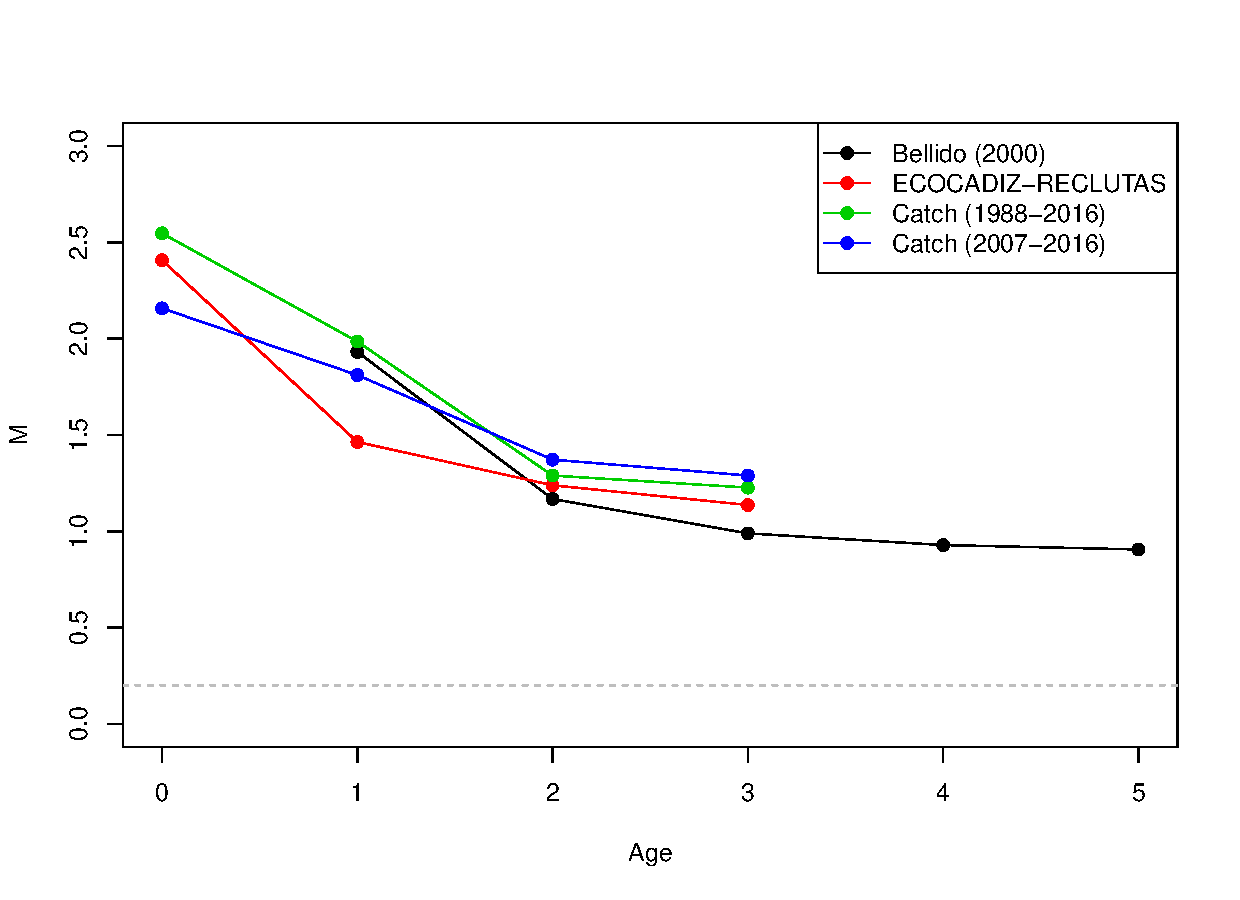
\includegraphics[bb=0 0 595 288]{./Natmort.pdf}
%  % lendist.pdf: 667x841 pixel, 72dpi, 23.53x29.67 cm, bb=0 0 667 841
%  \caption{Estimated natural mortality using Gislason approach and different reference time series to calculate length at age relationship}
%  \label{Natmort}
% \end{figure}





%inverse of SS for each component as weight and then this run is compared with those from the iterative reweighting scheme of \citet{stefansson_comparing_1998,stefansson_issues_2003}. The general idea is to use the inverse variance of the residuals of the former comparison are assigned as weights .
% Modeling details can be found in the appendix.
%
%
%
%
%
% Sea surface temperature (SST), discharges from the Alcal{\'a} del R{\'i}o reservoir and wind from 1996 to 2004, were obtained as follows: SST was extracted from  the Advanced Very High Resolution Radiometer (AVHRR) sensor data. The nighttime AVHRR PATHFINDER SST v5 weekly means with $4 \times 4 \quad km^{2}$ pixel resolution were taken from NASA PO.DAAC website (http://podaac.jpl.nasa.gov/). The  region of interest was acquired from the global image and arithmetic means were calculated based on all pixels within this region. Discharges  were provided by Confederaci{\'o}n Hidrogr{\'a}fica del Guadalquivir. They correspond to the monthly accumulated cubic hectometers that are discharged from the reservoir each month. Wind data are the weekly accumulated time (in days) that easterlies faster than $30 \quad km h^{-1}$ have been recorded in the meteorological station of C{\'a}diz.
%
%
% obtained from public databases
% Historical records of environmental covariates
%
% Individuals that have survived for five months, % $B_{t,s}(5),$
% are  considered  recruits and  are included in the stock population size owing to their availability to the fishery. The fishery closes from November to February approximately each year to allow growth of individuals spawned from May to September \citep{ices2012}.
%
%
%
%
%
% Gadget implementation
% combines a large pool of data from diverse sources to diagnose the stock dynamics.
%
%
%
% In this section we give a general description of the %data,
% models and data used, as well as the
%
%
% models, and indicators upon which we \textit{have} focused. We have chosen %two
% \textit{some models used for the assessment of data poor stocks}
% %models, a data limited methods (DLMtool)
% and a Gadget model.
%
% % DLMtool is a free R software package for management strategy evaluation and implementation of data-limited fishery stock assessment methods. The simple models used in this case study are models previously developed for data-limited approaches. A user-friendly tool, the Data-Limited Methods Toolkit \url{http://www.datalimitedtoolkit.org}, recognizes which of the acceptable methods can be applied to the data for the stock and then implement them, eventually, estimating indicators.
%
% Gadget is a parametric and deterministic \textit{age-length-structured} forward population dynamics simulation model\textit{. It} %that
% estimates population dynamics parameters based on fisheries data %and allows the coupling of a model with
% \textit{allowing the use of} an extensive set of data comparison and optimisation routines. Gadget works by running \textit{several times} an internal model based on many parameters, and then comparing the data from the output of this model to observed data to get
% \textit{the best}
% %a
% goodness-of-fit
% %likelihood score
% %The parameters can then be adjusted, and the model re-run, until an optimum is found, which corresponds to the model with the lowest likelihood score. Each stock is de???ned by specifying the length groups, age groups, and length-weight relationship to be used, along with the functions required to simulate the biological processes that affect the stock
% \cite{begley&howell2005}. %Gadget models have been developed using a specialised R-package, Rgadget.
% The standard model and the detail of the general model are described in \cite{begley2004gadget} and in \cite{taylor2007simple}.
%
% DLMtool is a free R software package for management strategy evaluation and implementation of data-limited fishery stock assessment methods. The simple models used in this case study are models previously developed for data-limited approaches. A user-friendly tool, the Data-Limited Methods Toolkit \url{http://www.datalimitedtoolkit.org}, recognizes which of the acceptable methods can be applied to the data for the stock and then implement them, eventually, estimating indicators.

%The comparisons across models must be based on value resulting from the estimates, which are called indicators. The indicators were calculated based on the output produced by the models. All the models estimate indicators with different approach to calculate the TAC value. The value obtained were then used to perform model comparisons. We focus upon two comparisons, one using real data and one using a MSE approach with simulated data.


\section{Fit to data}

A summary of likelihood scores is presented in Figure \ref{like} while a comparison of estimated versus observed data is summarized in the following Figures:

\subsubsection*{Length distributions}
\begin{itemize}
\item Figure \ref{lendist}: Length distribution of the commercial fleet.
\item Figure \ref{ecodist}: Length distribution of the ECOCADIZ acoustic survey. 
\item Figure \ref{peldist}: Length distribution of the PELAGO acoustic survey.
%\item Figure \ref{arsadist}: Length distribution of the ARSA bottom trawl survey.
\item Figure \ref{resildist}: Summary of residuals for length distributions.
\end{itemize}
\subsubsection*{Age distributions}
\begin{itemize}
\item Figure \ref{agedist}: Age distribution of the commercial fleet.
\item Figure \ref{ecoagedist}: Age distribution of the ECOCADIZ acoustic survey. 
%\item Figure \ref{ecorecdist}: Age distribution of the ECOCADIZ-RECLUTAS acoustic survey.
\item Figure \ref{pelagedist}: Age distribution of the PELAGO acoustic survey.
\item Figure \ref{resialdist}: Summary of residuals for age distributions.
\end{itemize}


% \subsubsection*{Age-length distributions}
% \begin{itemize}
% \item Figure \ref{alseine}: Fitted length at age by quarter compared to observed values from the spanish purse-seine samples
% \item Figure \ref{aleco}: Fitted length at age by quarter compared to observed values from the ECOCADIZ acoustic survey samples
% %\item Figure \ref{alecorec}: Fitted length at age by quarter compared to observed values from the ECOCADIZ-RECLUTAS acoustic survey samples
% \item Figure \ref{alpel}: Fitted length at age by quarter compared to observed values from the PELAGO acoustic survey samples
% \end{itemize}


\subsubsection*{Biomass survey indices fit}
\begin{itemize}
\item Figure \ref{surveyfit}: Summary of biomass survey indices fit. 
\end{itemize}

\begin{figure}[h!]
 \centering
 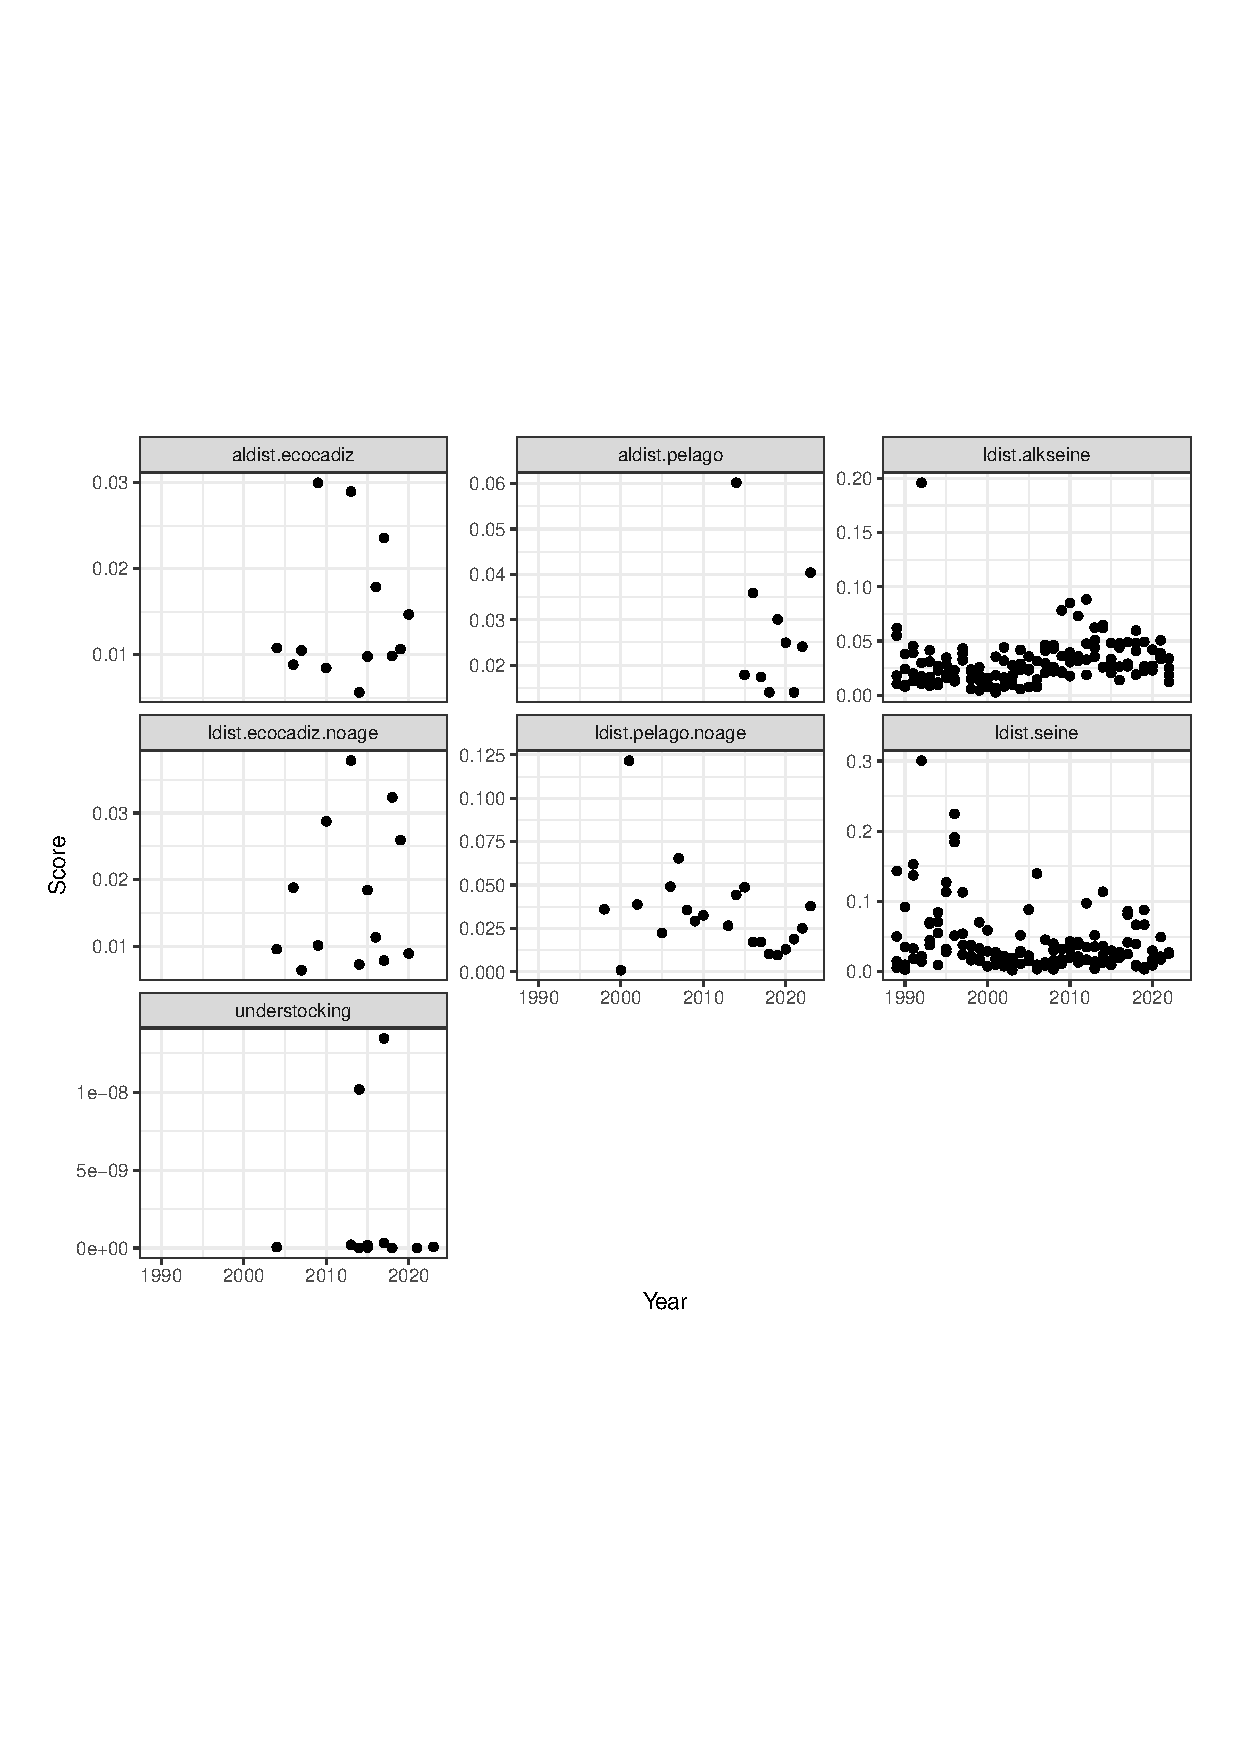
\includegraphics[bb=0 0 595 841]{./likelihood.pdf}
  \caption{Likelihood scores for age-length key of ECOCADIZ survey, PELAGO survey and commercial landings (Upper panel) and length distribution of ECOCADIZ survey, PELAGO survey and landings. Dots represent the score for each quarter.}
 \label{like}
 % likelihood.pdf: 523x379 pixel, 72dpi, 18.45x13.37 cm, bb=0 0 523 379
\end{figure}


% The following shows the  likelihood component scores from the different stages of the iterative reweighting run normalised with the minimum score for each component


\begin{figure}[h!]
 \centering
 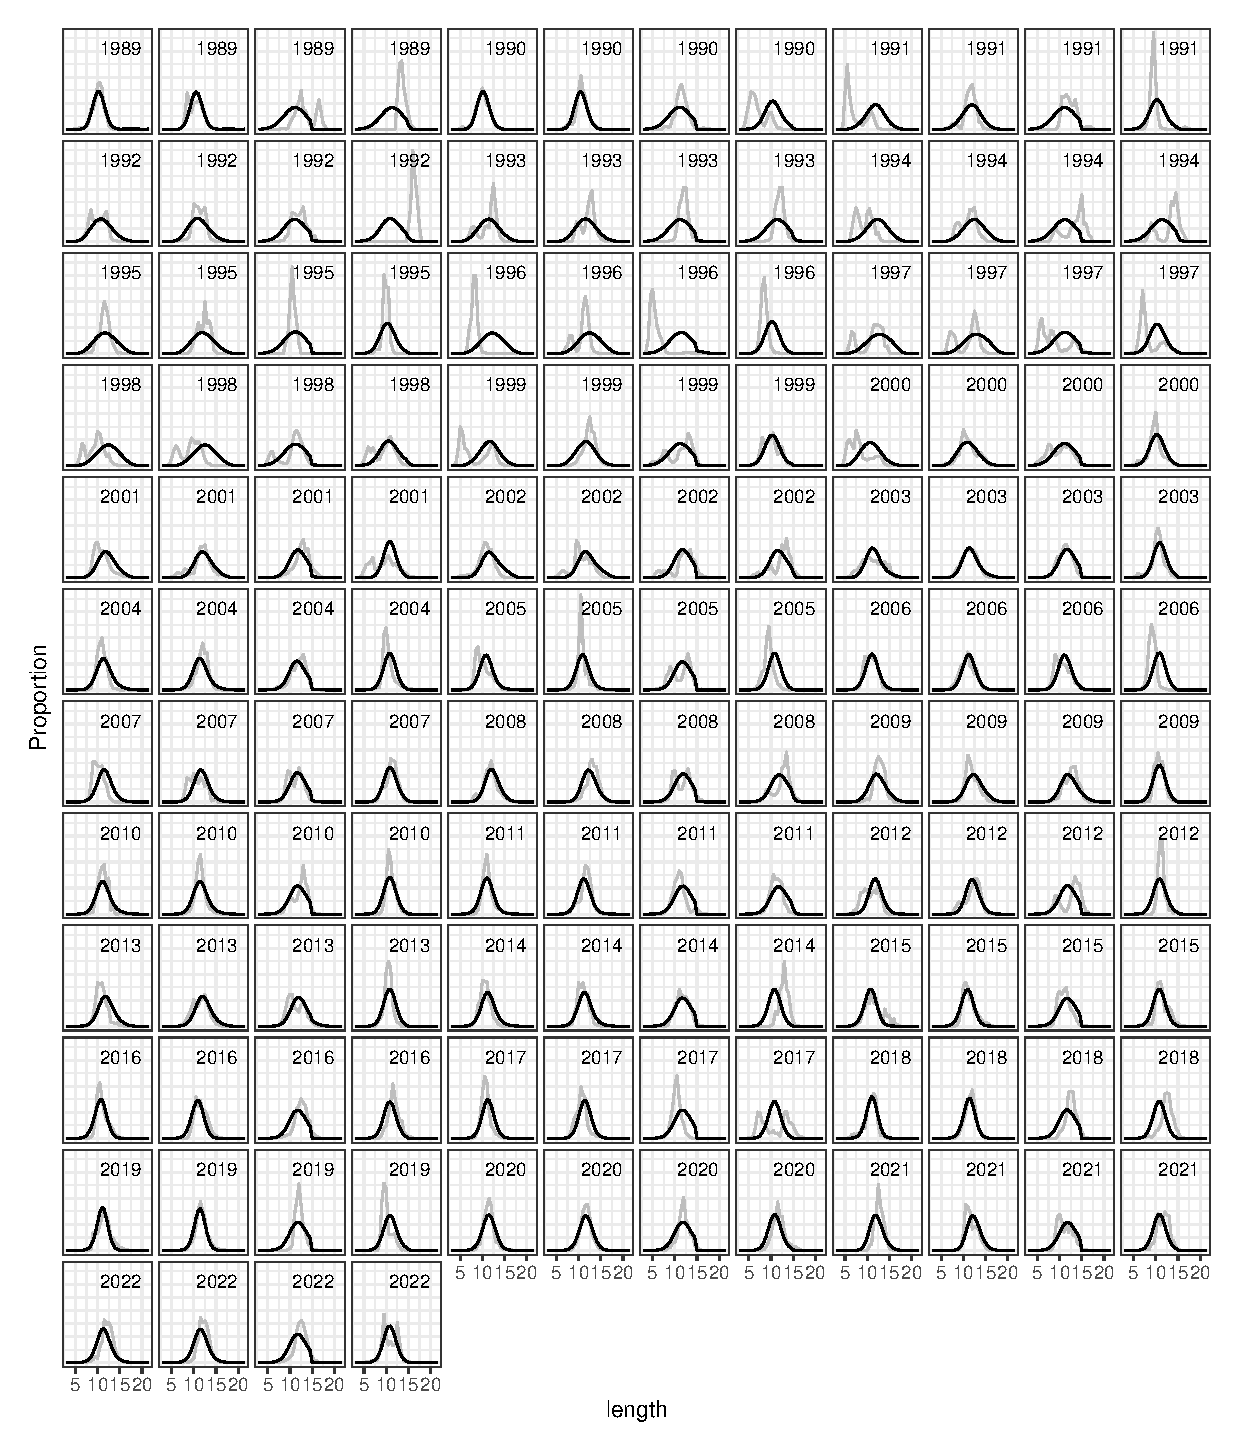
\includegraphics[bb=0 0 595 697]{./lendist.pdf}
 % lendist.pdf: 667x841 pixel, 72dpi, 23.53x29.67 cm, bb=0 0 667 841
 \caption{ Comparison between observed and estimated catches length distribution. Black lines represent estimated data while gray lines represent observed data}
 \label{lendist}
\end{figure}

\begin{figure}[h!]
 \centering
 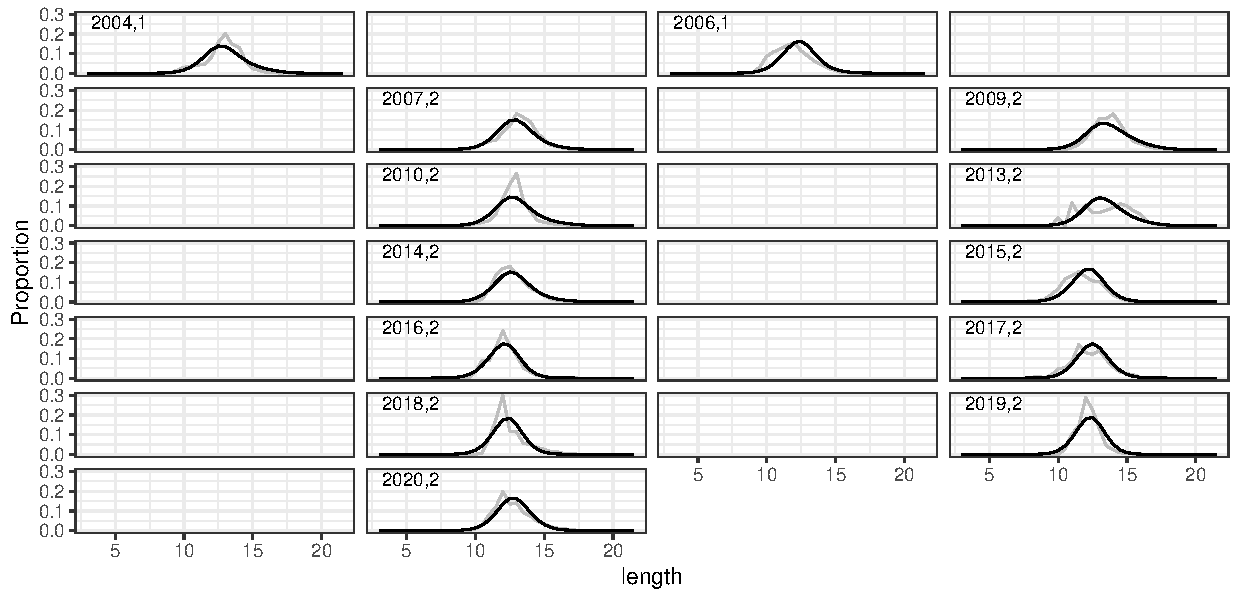
\includegraphics[bb=0 0 595 697]{./ecodist.pdf}
 % lendist.pdf: 667x841 pixel, 72dpi, 23.53x29.67 cm, bb=0 0 667 841
 \caption{ Comparison between observed and estimated catches length distribution for ECOCADIZ survey. Black lines represent estimated data while gray lines represent observed data}
 \label{ecodist}
\end{figure}

\begin{figure}[h!]
 \centering
 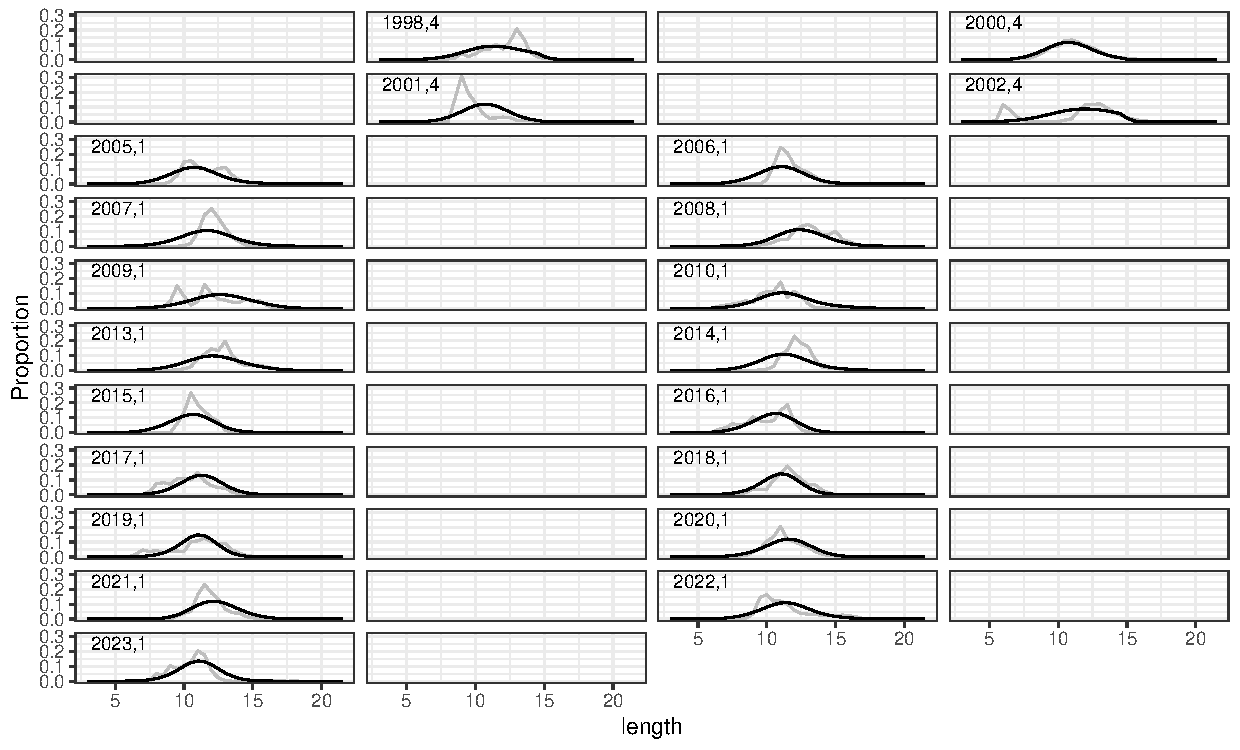
\includegraphics[bb=0 0 595 697]{./peldist.pdf}
 % lendist.pdf: 667x841 pixel, 72dpi, 23.53x29.67 cm, bb=0 0 667 841
 \caption{ Comparison between observed and estimated catches length distribution for PELAGO survey. Black lines represent estimated data while gray lines represent observed data}
 \label{peldist}
\end{figure}



% \begin{figure}[h!]
%  \centering
%  \includegraphics[bb=0 0 595 504]{./arsadist.pdf}
%  % lendist.pdf: 667x841 pixel, 72dpi, 23.53x29.67 cm, bb=0 0 667 841
%  \caption{ Comparison between observed and estimated ARSA bottom trawl survey length distribution. Black lines represent estimated data while gray lines represent observed data}
%  \label{arsadist}
% \end{figure}


\begin{figure}[h!]
 \centering
 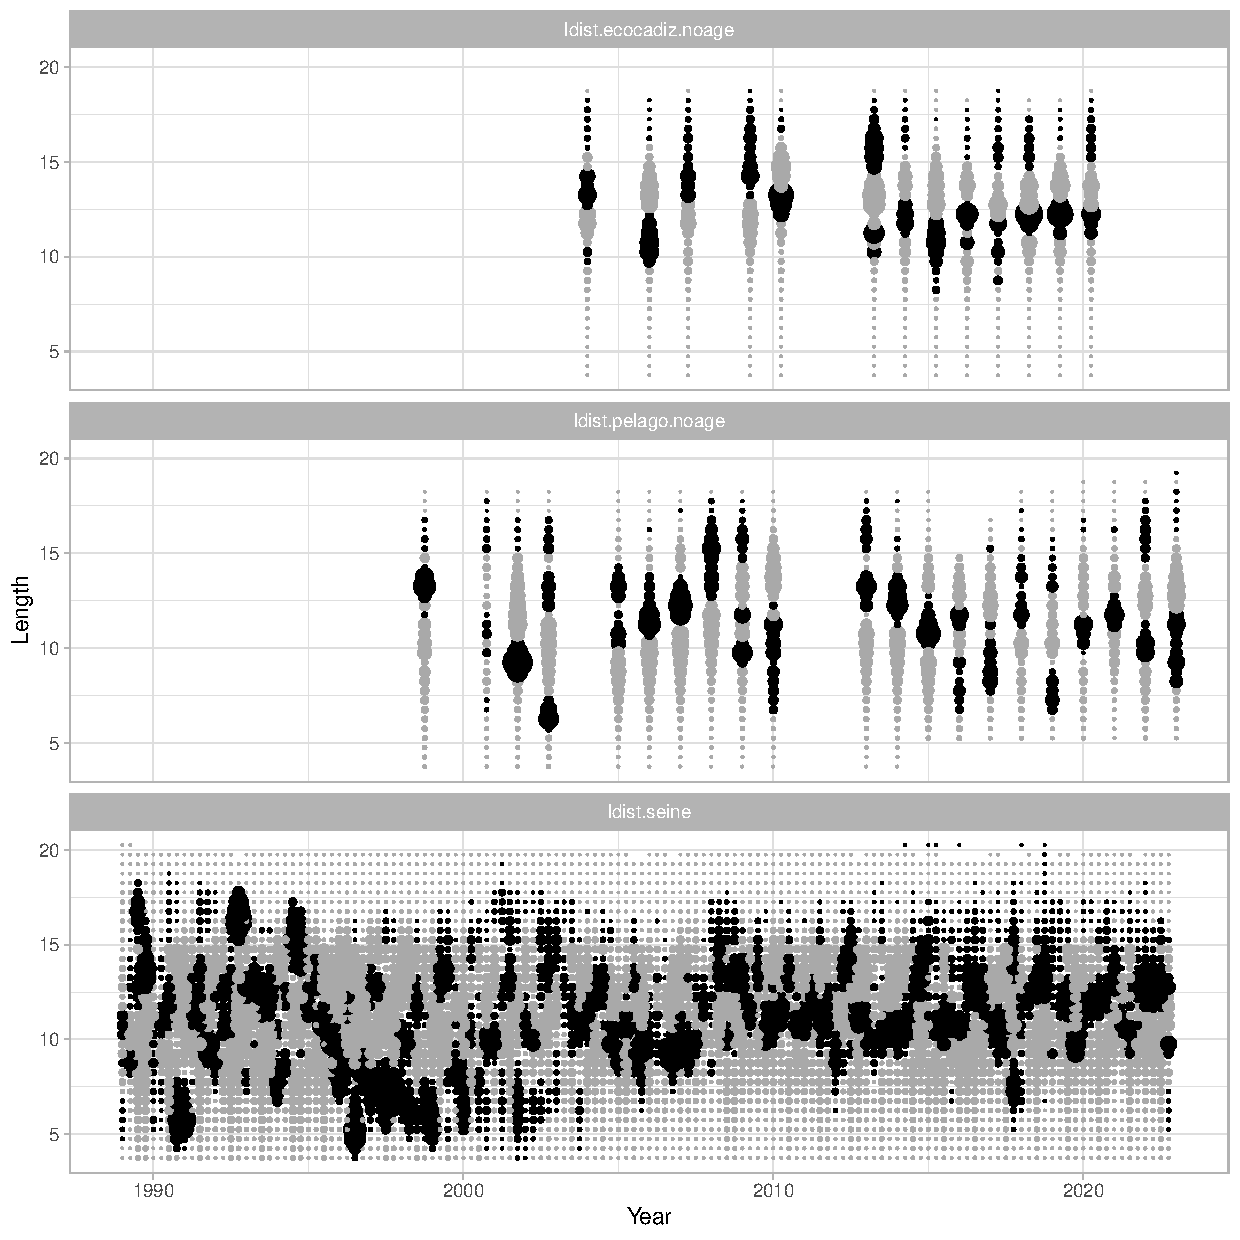
\includegraphics{./resildist.pdf}
 %lendist.pdf: 667x841 pixel, 72dpi, 23.53x29.67 cm, bb=0 0 667 841
 \caption{ Standardised residual plots for the fitted length distribution
from the ECOCADIZ survey, PELAGO survey and commercial landings. Black points denote a model underestimate and
gray points an overestimated. The size of the points denote the scale of the standardised
residual.}
 \label{resildist}
\end{figure}





\begin{figure}
\centering
 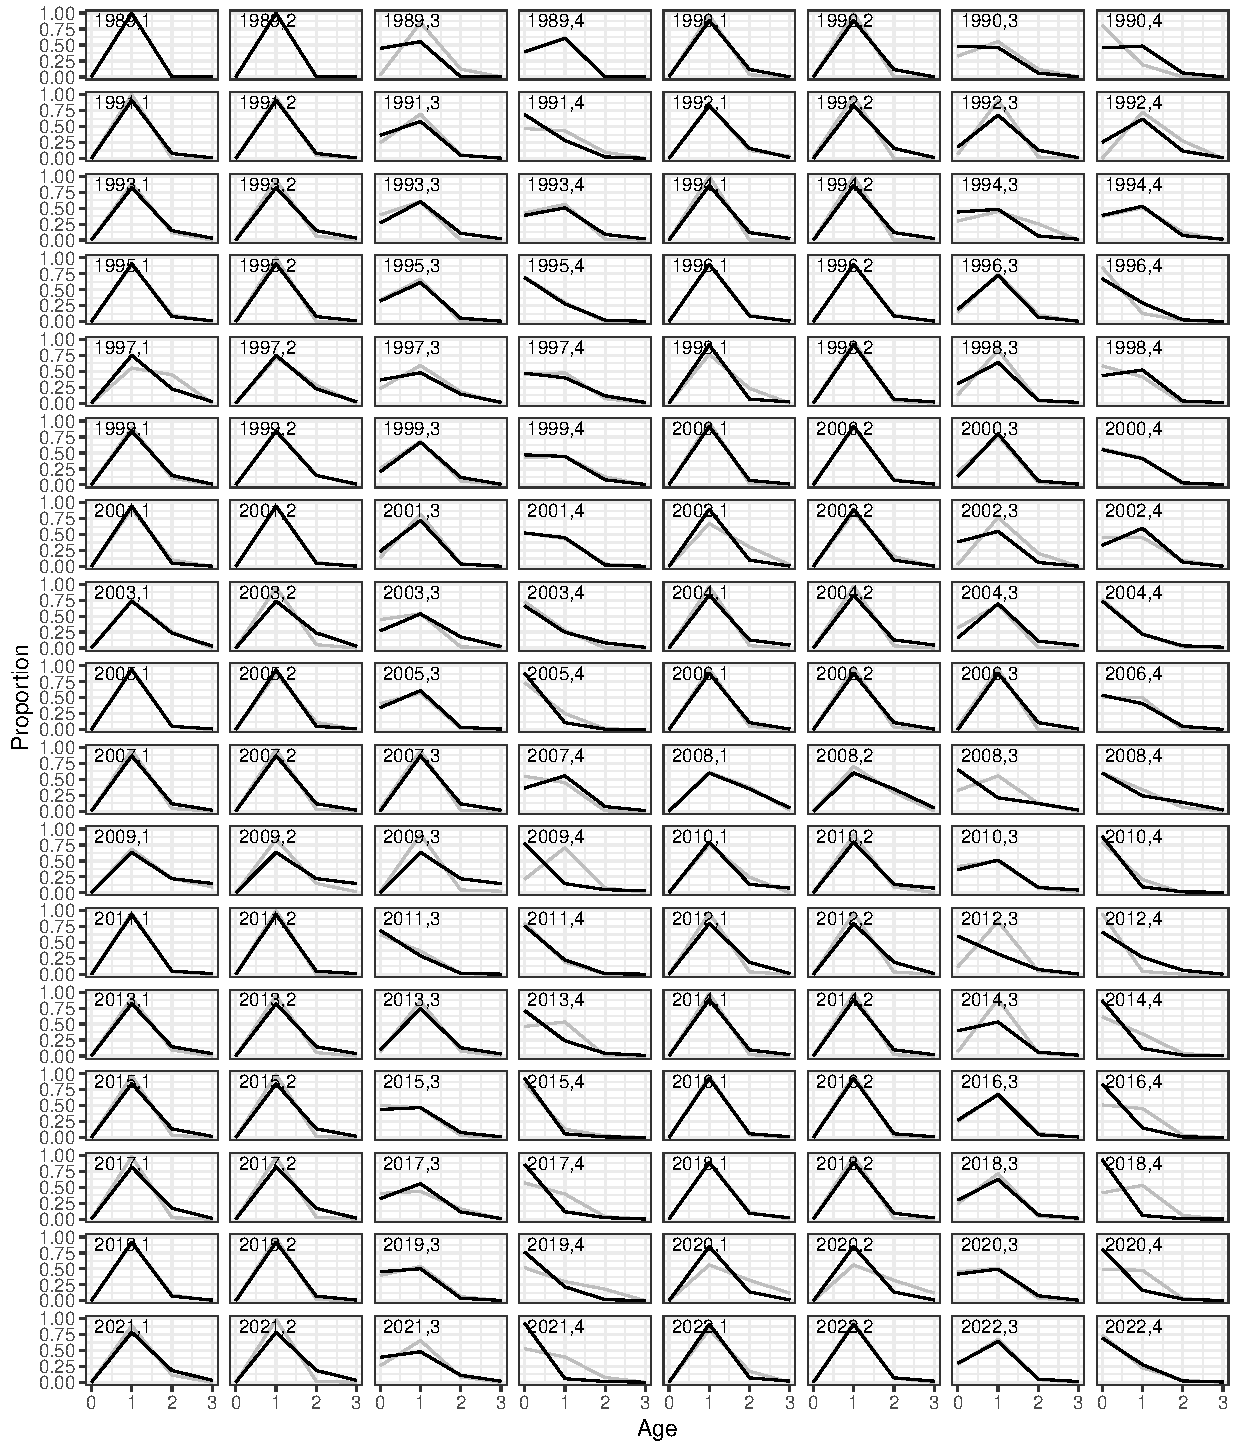
\includegraphics[bb=0 0 595 697]{./agedist.pdf}
 % agedist.pdf: 667x841 pixel, 72dpi, 23.53x29.67 cm, bb=0 0 667 841
 \caption{ Comparison between observed and estimated catches age distribution. Black lines represent estimated data while gray lines represent observed data.}
 \label{agedist}
\end{figure}

\begin{figure}
\centering
 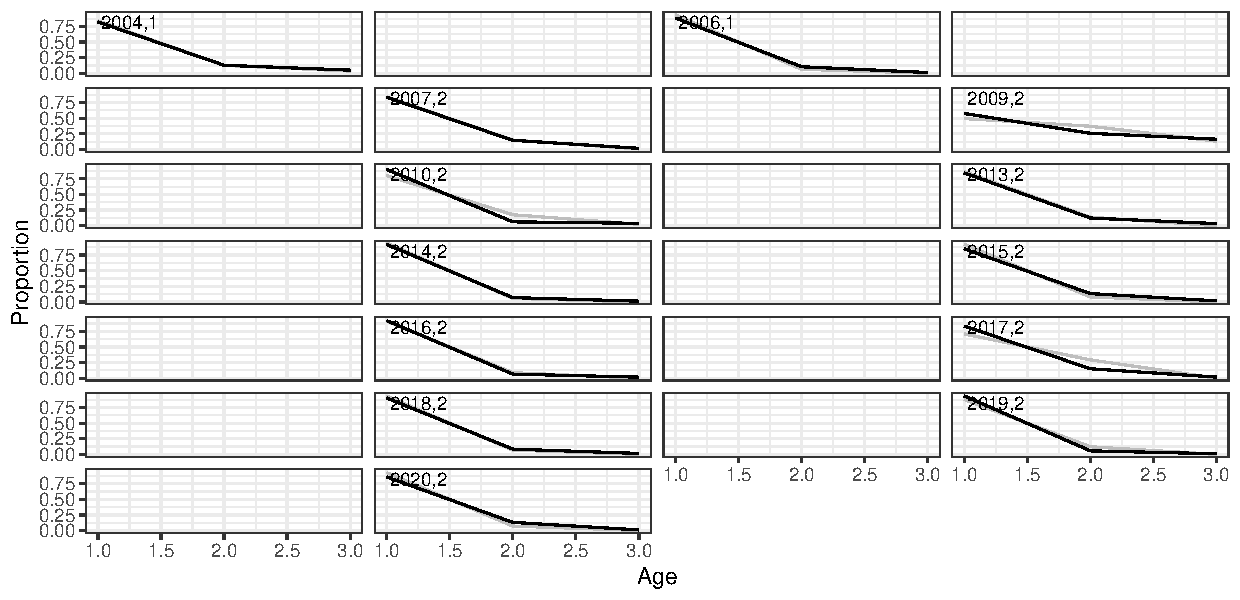
\includegraphics[bb=0 0 595 288]{./ecoagedist.pdf}
 % agedist.pdf: 667x841 pixel, 72dpi, 23.53x29.67 cm, bb=0 0 667 841
 \caption{ Comparison between observed and estimated ECOCADIZ survey age distribution. Black lines represent estimated data while gray lines represent observed data.}
 \label{ecoagedist}
\end{figure}


% \begin{figure}
% \centering
%  \includegraphics[bb=0 0 595 144]{./ecorecdist.pdf}
%  % agedist.pdf: 667x841 pixel, 72dpi, 23.53x29.67 cm, bb=0 0 667 841
%  \caption{ Comparison between observed and estimated ECOCADIZ-RECLUTAS survey age distribution. Black lines represent estimated data while gray lines represent observed data.}
%  \label{ecorecdist}
% \end{figure}


\begin{figure}
\centering
 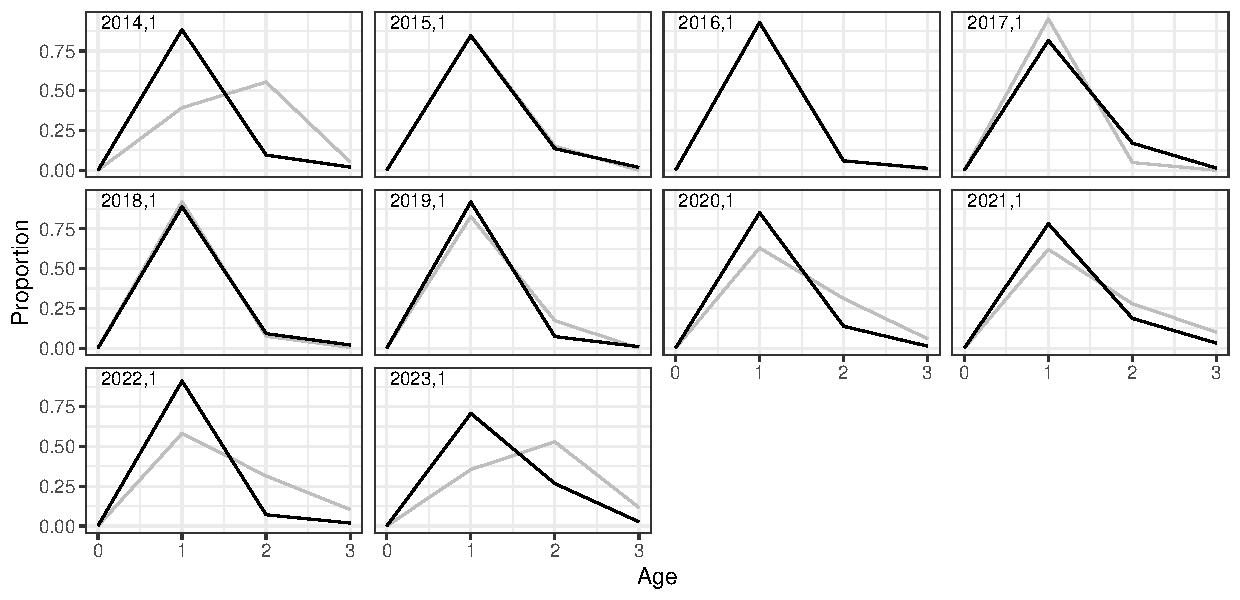
\includegraphics[bb=0 0 595 360]{./pelagedist.pdf}
 % agedist.pdf: 667x841 pixel, 72dpi, 23.53x29.67 cm, bb=0 0 667 841
 \caption{ Comparison between observed and estimated PELAGO survey age distribution. Black lines represent estimated data while gray lines represent observed data.}
 \label{pelagedist}
\end{figure}


% \begin{figure}
% \centering
%  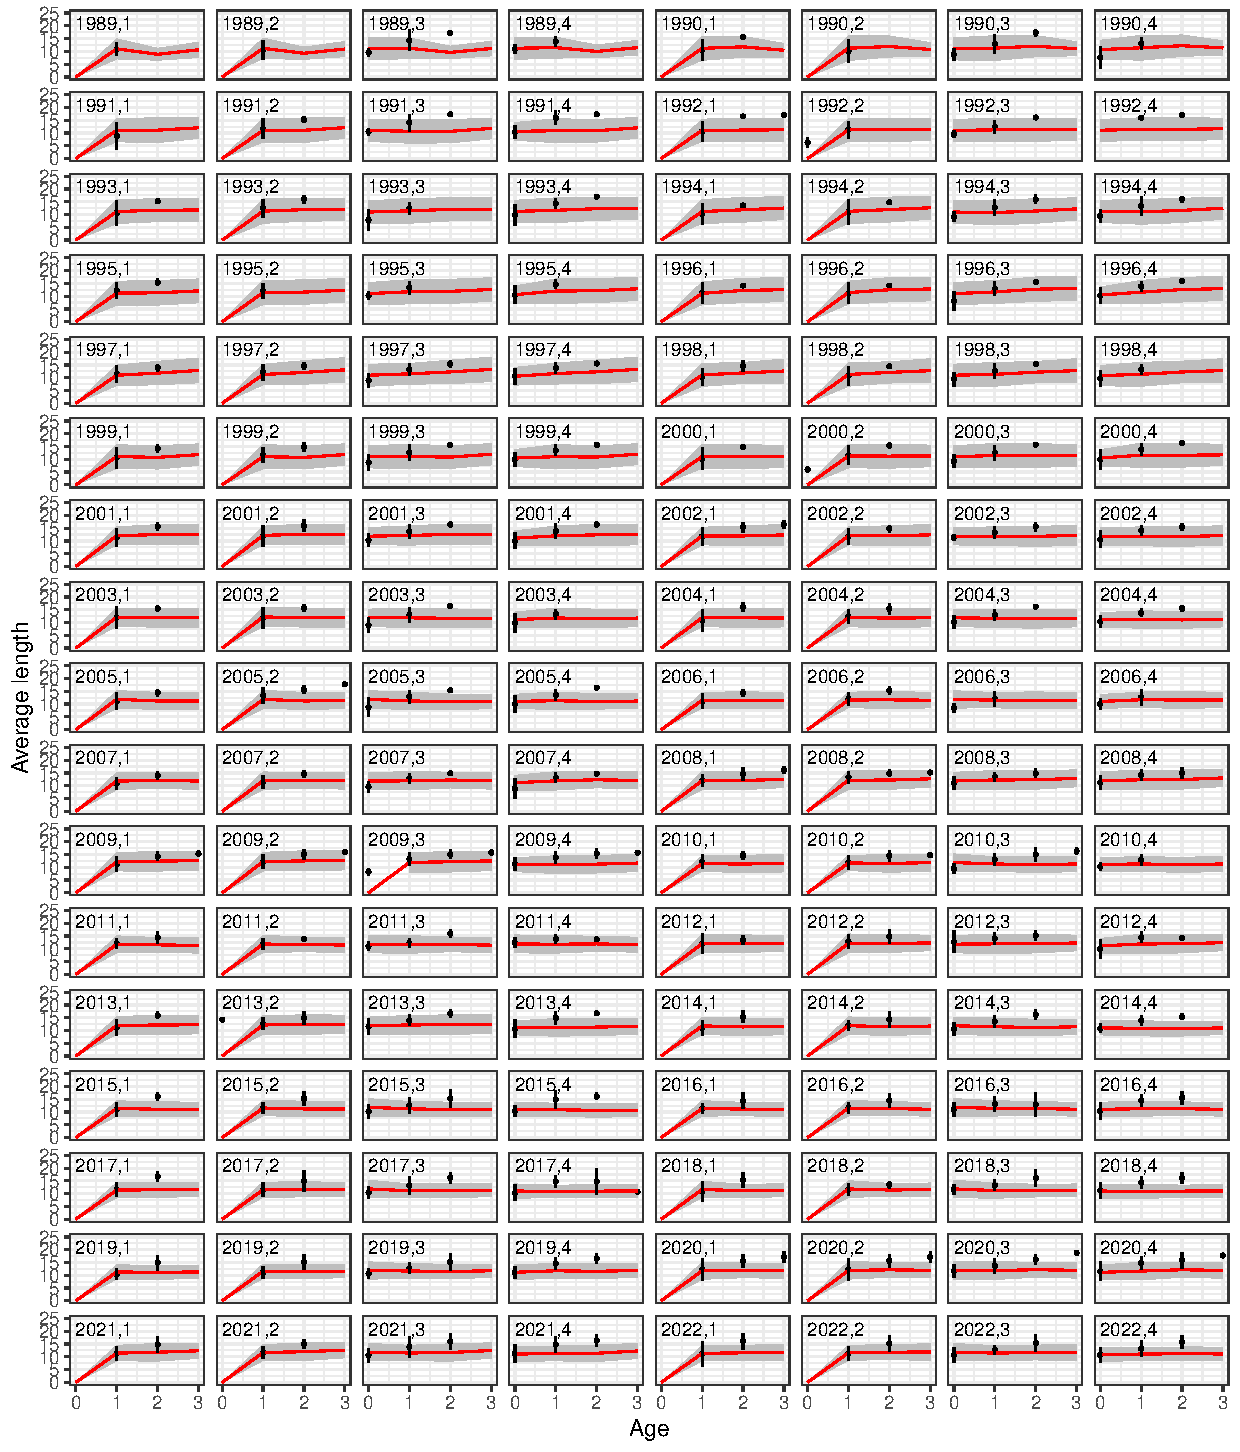
\includegraphics[bb=0 0 595 697]{./alseine.pdf}
%  % agedist.pdf: 667x841 pixel, 72dpi, 23.53x29.67 cm, bb=0 0 667 841
%  \caption{Fitted length at age by quarter compared to observed values from the spanish purse-seine samples. The black point and vertical bar denotes the observed mean and 95\% confidence intervals of length at age, while the grey ribbon and red line indicates the model estimates.}
%  \label{alseine}
% \end{figure}

% \begin{figure}
% \centering
%  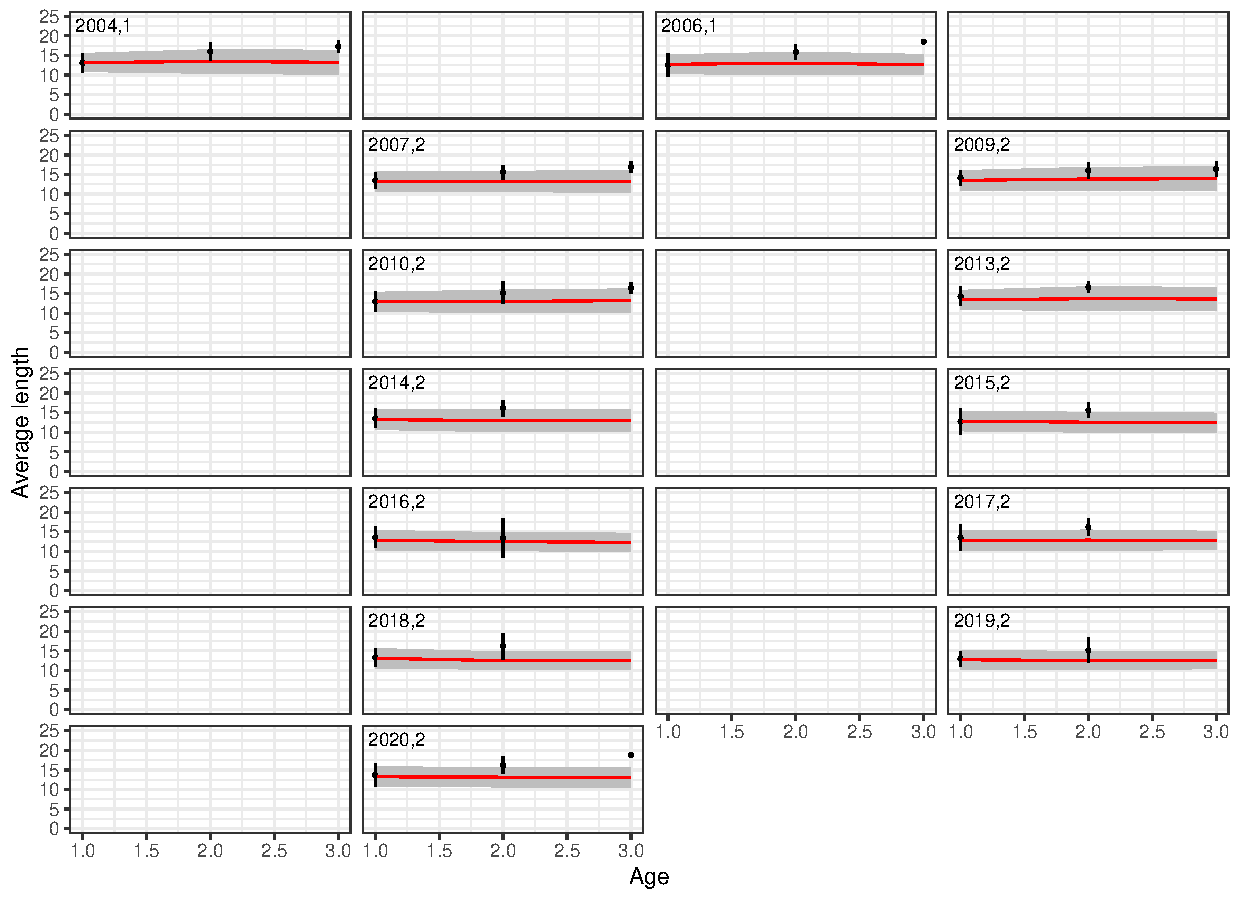
\includegraphics[bb=0 0 595 697]{./aleco.pdf}
%  % agedist.pdf: 667x841 pixel, 72dpi, 23.53x29.67 cm, bb=0 0 667 841
%  \caption{Fitted length at age by quarter compared to observed values from the ECOCADIZ survey samples. The black point and vertical bar denotes the observed mean and 95\% confidence intervals of length at age, while the grey ribbon and red line indicates the model estimates.}
%  \label{aleco}
% \end{figure}

% \begin{figure}
% \centering
%  \includegraphics[bb=0 0 595 697]{./alecorec.pdf}
%  % agedist.pdf: 667x841 pixel, 72dpi, 23.53x29.67 cm, bb=0 0 667 841
%  \caption{Fitted length at age by quarter compared to observed values from the ECOCADIZ-RECLUTAS survey samples. The black point and vertical bar denotes the observed mean and 95\% confidence intervals of length at age, while the grey ribbon and red line indicates the model estimates.}
%  \label{alecorec}
% \end{figure}

% \begin{figure}
% \centering
%  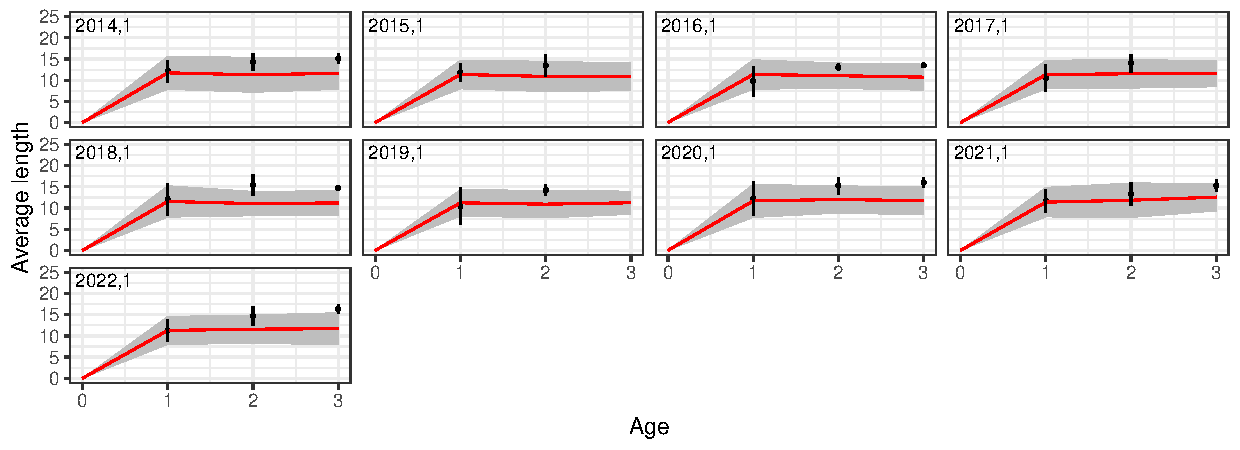
\includegraphics[bb=0 0 595 697]{./alpel.pdf}
%  % agedist.pdf: 667x841 pixel, 72dpi, 23.53x29.67 cm, bb=0 0 667 841
%  \caption{Fitted length at age by quarter compared to observed values from the PELAGO survey samples. The black point and vertical bar denotes the observed mean and 95\% confidence intervals of length at age, while the grey ribbon and red line indicates the model estimates.}
%  \label{alpel}
% \end{figure}

\begin{figure}
\centering
 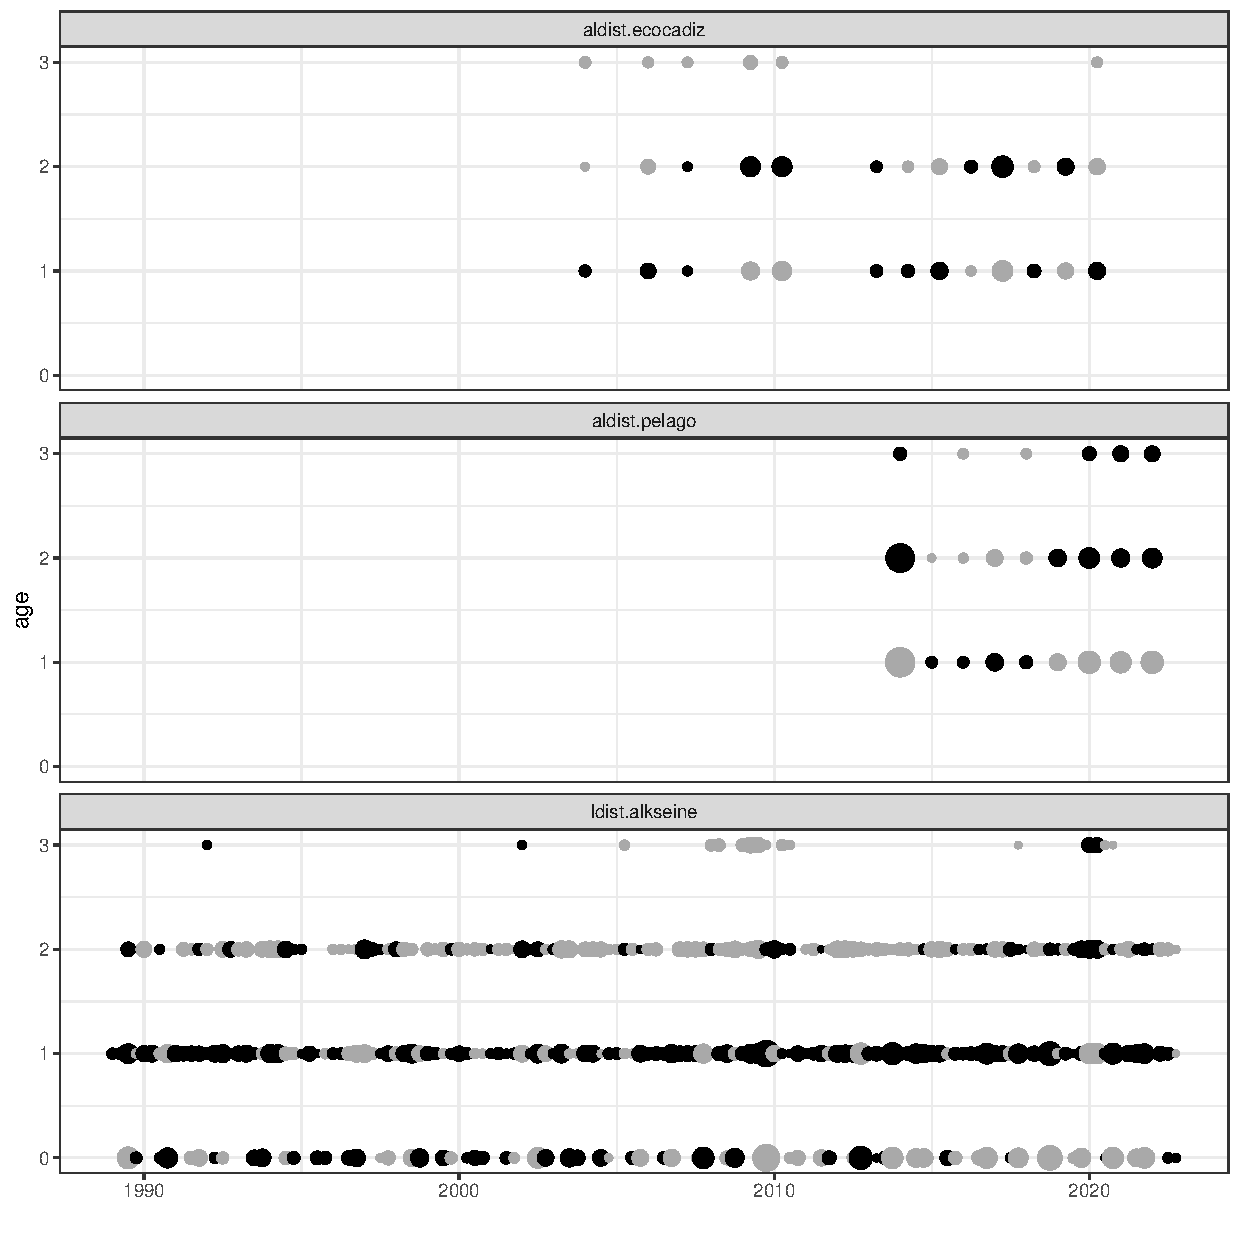
\includegraphics{./resialdist.pdf}
 % agedist.pdf: 667x841 pixel, 72dpi, 23.53x29.67 cm, bb=0 0 667 841
 \caption{ Standardised residual plots for the fitted age distribution
from the ECOCADIZ survey, PELAGO survey and commercial fleet. Black points denote a model underestimate and
gray points an overestimated. The size of the points denote the scale of the standardised
residual.}
 \label{resialdist}
\end{figure}


\begin{figure}[h!]
 \centering
 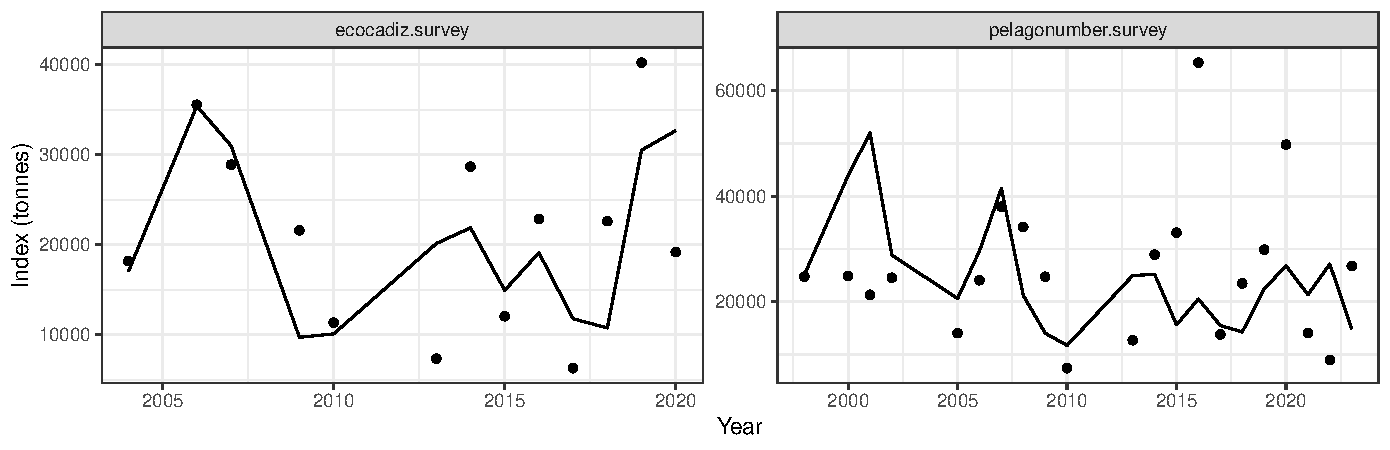
\includegraphics[bb=0 0 667 432]{./surveyfit.pdf}
 % lendist.pdf: 667x841 pixel, 72dpi, 23.53x29.67 cm, bb=0 0 667 841
 \caption{ Comparison between observed and estimated survey indices. Black points represent observed data while black line represent estimated data}
 \label{surveyfit}
\end{figure}

\clearpage
\section{Model estimates}

Parameter estimates after optimization are presented in Table \ref{Symbols}. Detailed model outputs are available in \href{https://github.com/ices-taf/2022_ane.27.9a_assessment/tree/main/results}{Results folder on TAF repository}, where each file corresponds to the following description:
\begin{itemize}
\item{sidat: }{Model fit to the surveyindices}
\item{suitability: }{Model estimated fleet suitability}
\item{stock.recruitment: }{Model estimated recruitment }
\item{res.by.year: }{Results by year}
\item{catchdist.fleets: }{Data compared with model output for the length and age-length distributions}
\item{stock.full: }{Modeled abundance and mean weight by year,step, length and stock}
\item{stock.std: }{Modeled abundance, mean weight, number by age consumed by the fleet, stock and year}
\item{stock.prey: }{Consumption of the fleet by length, year and step}
\item{fleet.info: }{Information on catches, harvest rate and harvestable biomass by fleet, year and step}
\item{params: }{parameter values used for the fit}
\end{itemize}




\subsection{Catchability}

Figure \ref{catchability} shows the catchability estimated by the model for the different surveys indices

\begin{figure}[h!]
 \centering
 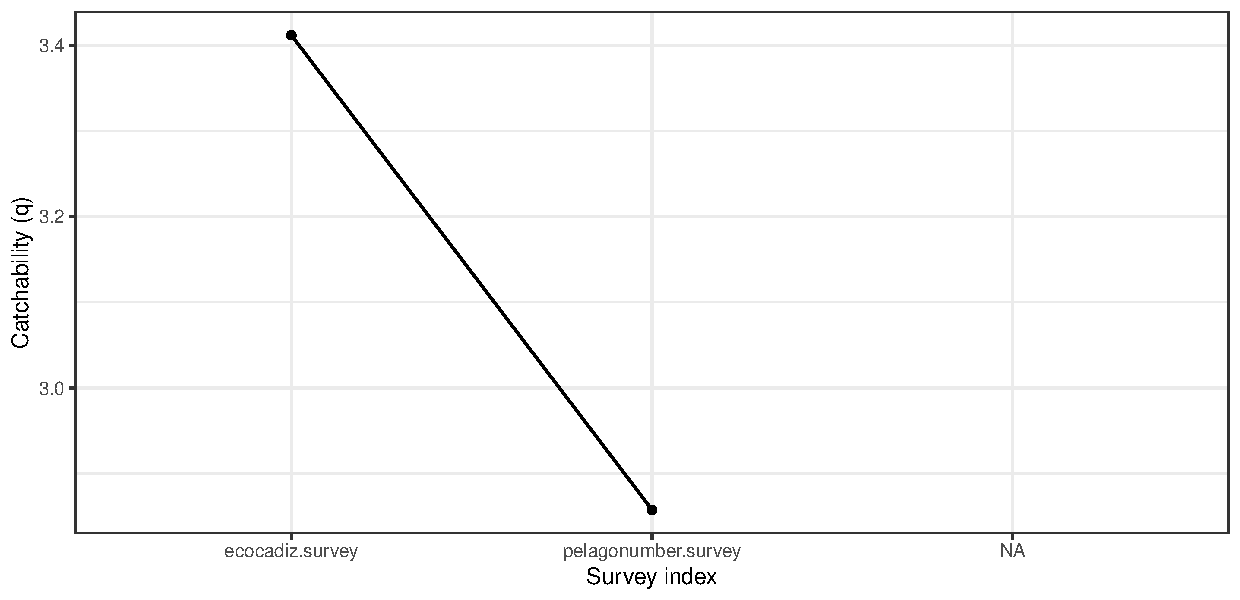
\includegraphics[bb=0 0 595 288]{./catchability.pdf}
 % lendist.pdf: 667x841 pixel, 72dpi, 23.53x29.67 cm, bb=0 0 667 841
 \caption{Estimated catchability parameters for the different survey indices}
 \label{catchability}
\end{figure}

\subsection{Estimated age composition}

Figure \ref{cohortevol} shows the estimated age composition of the population.
\begin{figure}[h!]
 \centering
 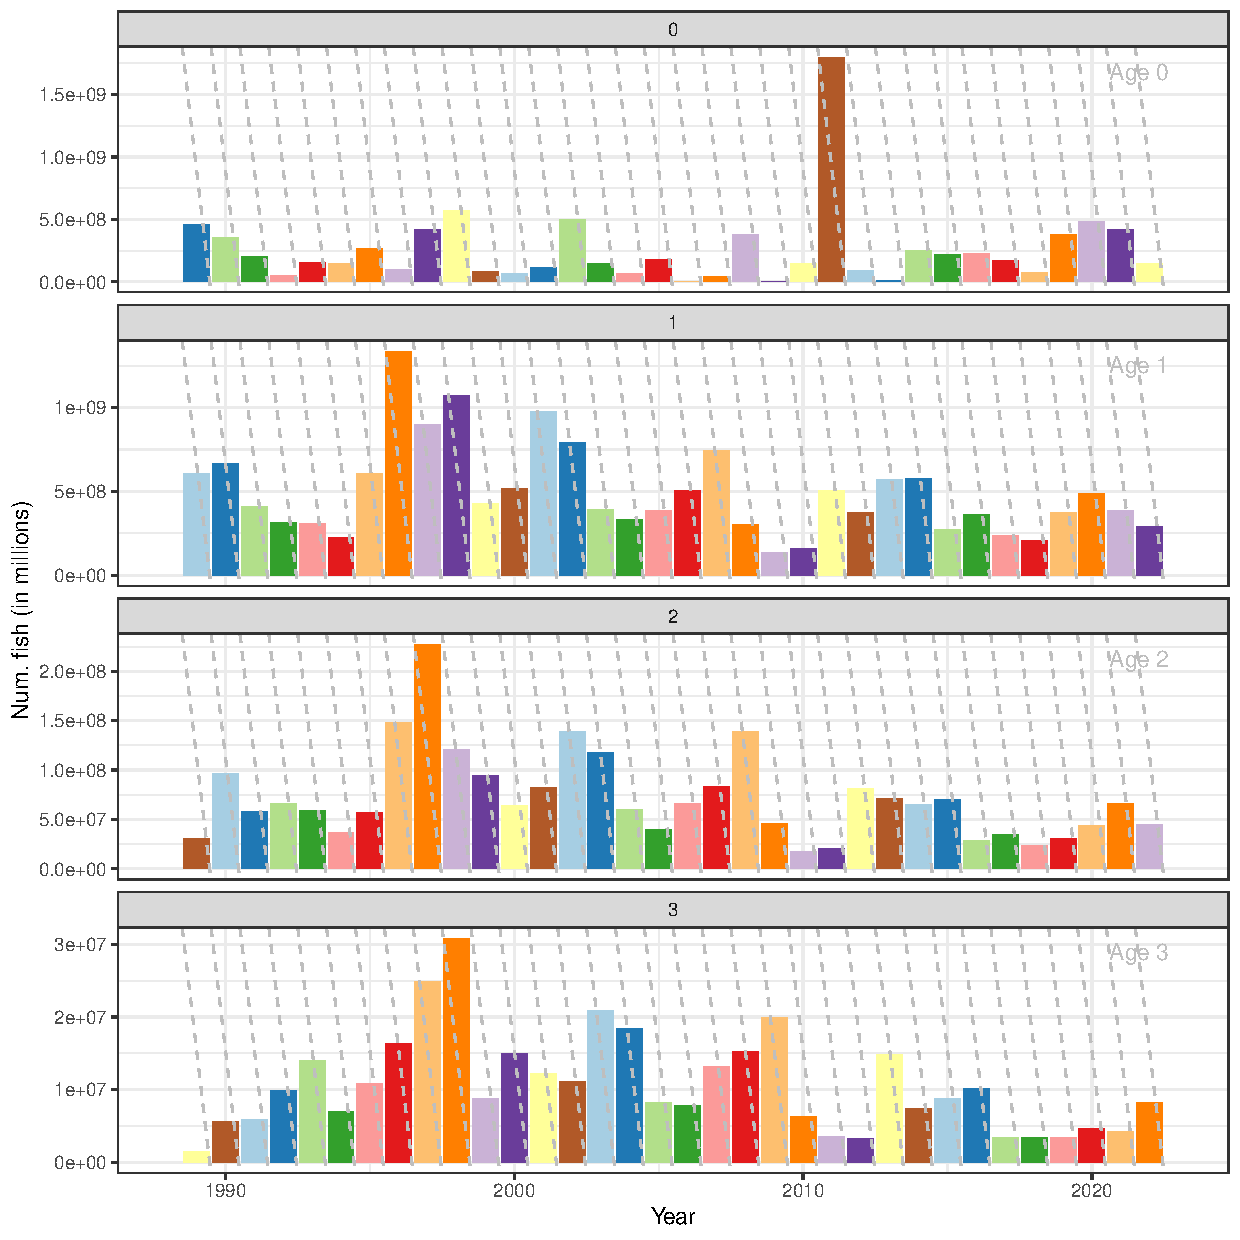
\includegraphics{./cohortevol.pdf}
 % lendist.pdf: 667x841 pixel, 72dpi, 23.53x29.67 cm, bb=0 0 667 841
 \caption{Estimated age composition of the population at the end of the second quarter for each year}
 \label{cohortevol}
\end{figure}

\subsection{Suitability}

Figure \ref{suitability} shows the fleet suitability functions estimated by the model for the commercial fleet and different surveys 
\begin{figure}[h!]
 \centering
 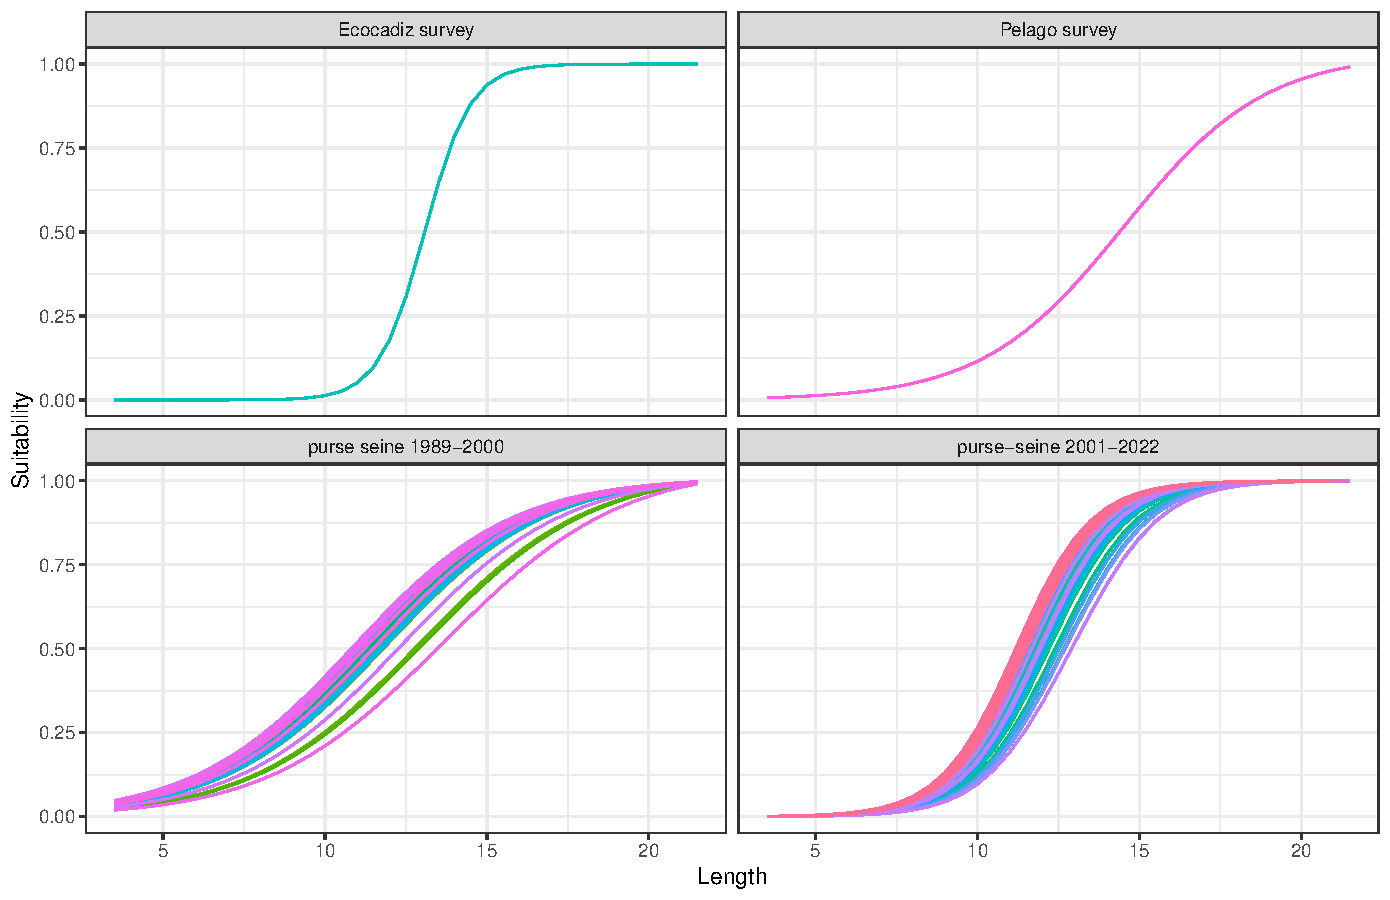
\includegraphics[bb=0 0 667 432]{./suitability.pdf}
 % lendist.pdf: 667x841 pixel, 72dpi, 23.53x29.67 cm, bb=0 0 667 841
 \caption{Estimated fleet suitability functions for the commercial fleet and different surveys.}
 \label{suitability}
\end{figure}



\subsection{Abundance, recruitment and Fishing mortality}\label{ARF}

Figure \ref{ICESplot} presents model annual estimates for biomass, abundance (removing age 0 individuals to be accurate with the time of the assessment, see section \ref{Remark} above for a detailed explanation), recruitment, fishing mortality and catches \textbf{at the end of the second quarter of each year}. Figure \ref{biomassts} shows annual estimates for biomass of individuals of age $1+$ at the end of the second quarter of each year. Due to some inconsistencies in the maturity ogives not noticed during WKPELA 2018, we assume that all individuals with age 1 or higher ($B_1+$), are mature i.e. these abundance estimates result equivalent to spawning stock biomass estimates.

\begin{figure}[h!]
 \centering
 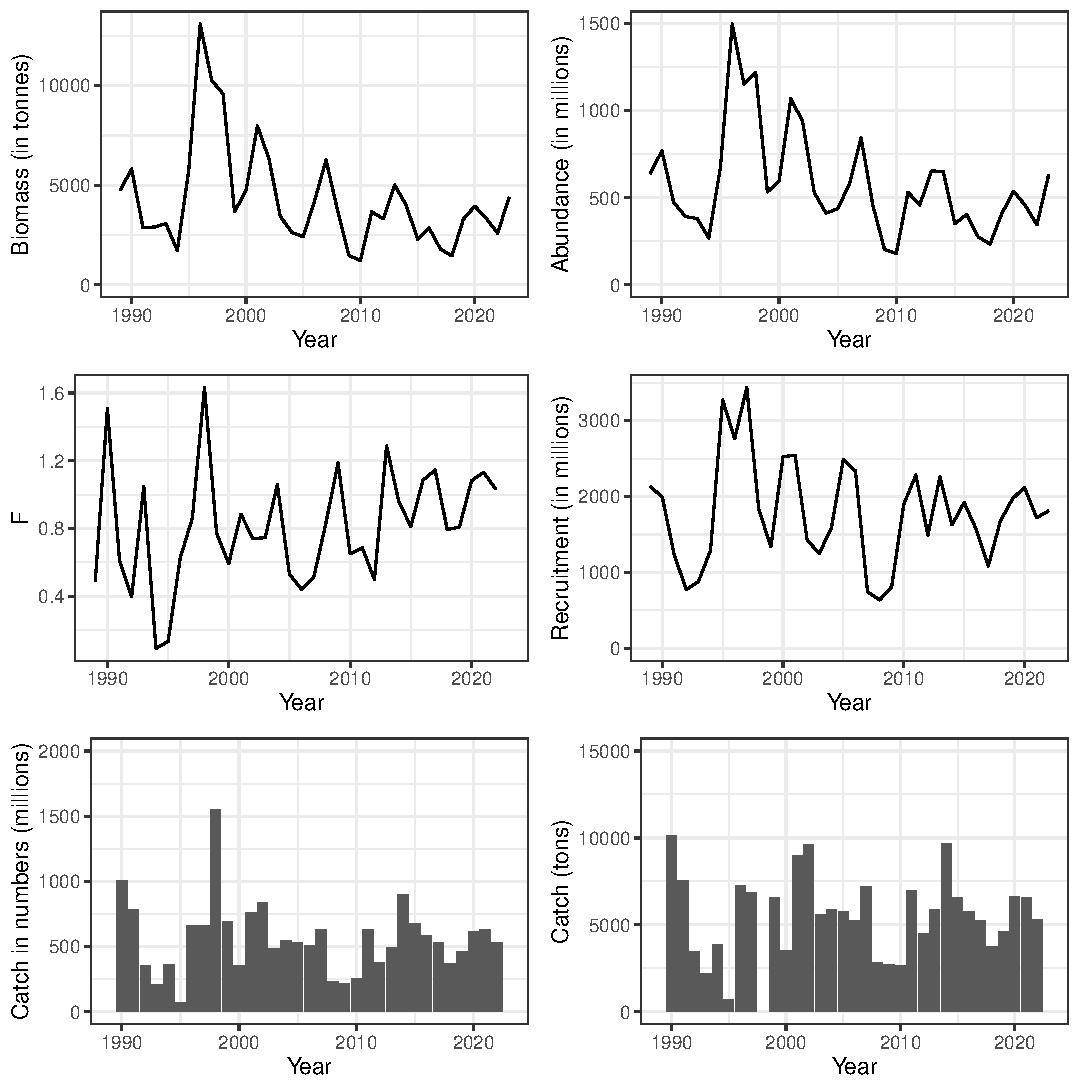
\includegraphics[bb=0 0 518 523]{./ICESplots.pdf}
 \caption{Annual catches time series (in numbers and biomass) compared with annual model estimates for abundance of individuals with more than one year of age(in numbers and biomass) recruitment and fishing mortality. Measures were summarized at the end of June each year, assuming that a year starts in July and ends in June of the next year. Recruitment was calculated including all the recruits of the previous year according to calendar year}
 \label{ICESplot}
 % ICESplots.pdf: 523x379 pixel, 72dpi, 18.45x13.37 cm, bb=0 0 523 379
\end{figure}
\begin{figure}[h!]
 \centering
 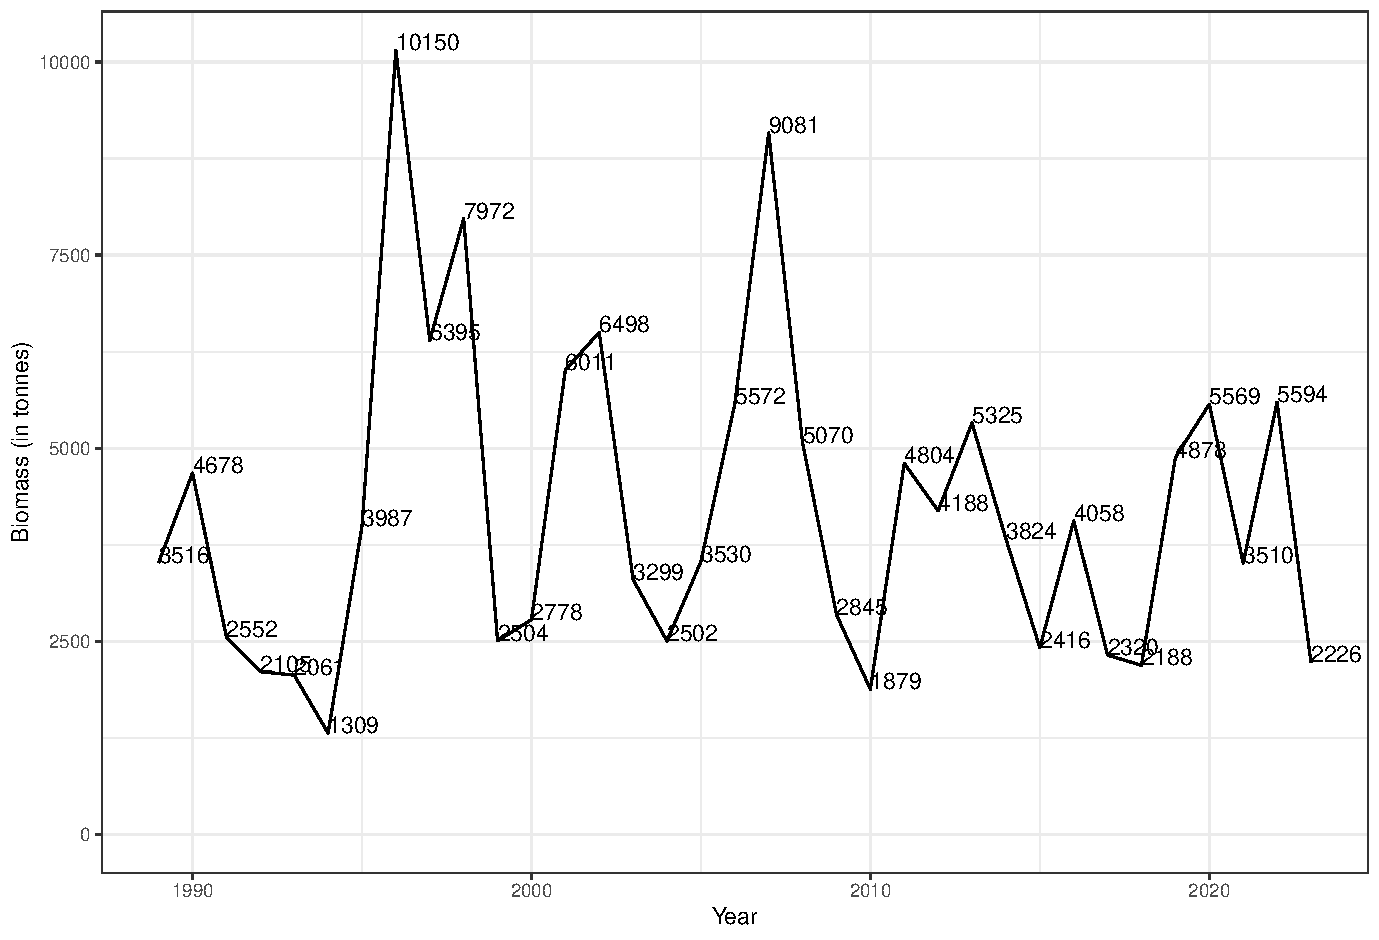
\includegraphics[bb=0 0 662 451]{./biomassts.pdf}
 % lendist.pdf: 667x841 pixel, 72dpi, 23.53x29.67 cm, bb=0 0 667 841
 \caption{Estimated biomass time series at the end of quarter two (Age 0 removed to be consistent with recruitment at the end of the second quarter of the year). Note that under the assumption that all individuals in $B1+$ class are mature, this biomass is equivalent to SSB}
 \label{biomassts}
\end{figure}

\subsection{Comparison with the last two years estimated time series}

A comparison with the last two years estimated time series is presented in Figure \ref{modelcomp}. The pink line represents the current year estimated time series (the one estimated by the model described in this document), the green line, the estimated in 2022 and the blue line, the estimated in 2021. Trends are consistent even considering that each year the model updates the last values with the new information available. %It was observed that the estimated biomass for some of the last years is smaller when including the length distribution missing (green line) but population trend remains very similar. It is also important to remark that the number of iterations for the optimization process in the first model was 2000000, while in the others was just 1000000.

\begin{figure}[h!]
 \centering
 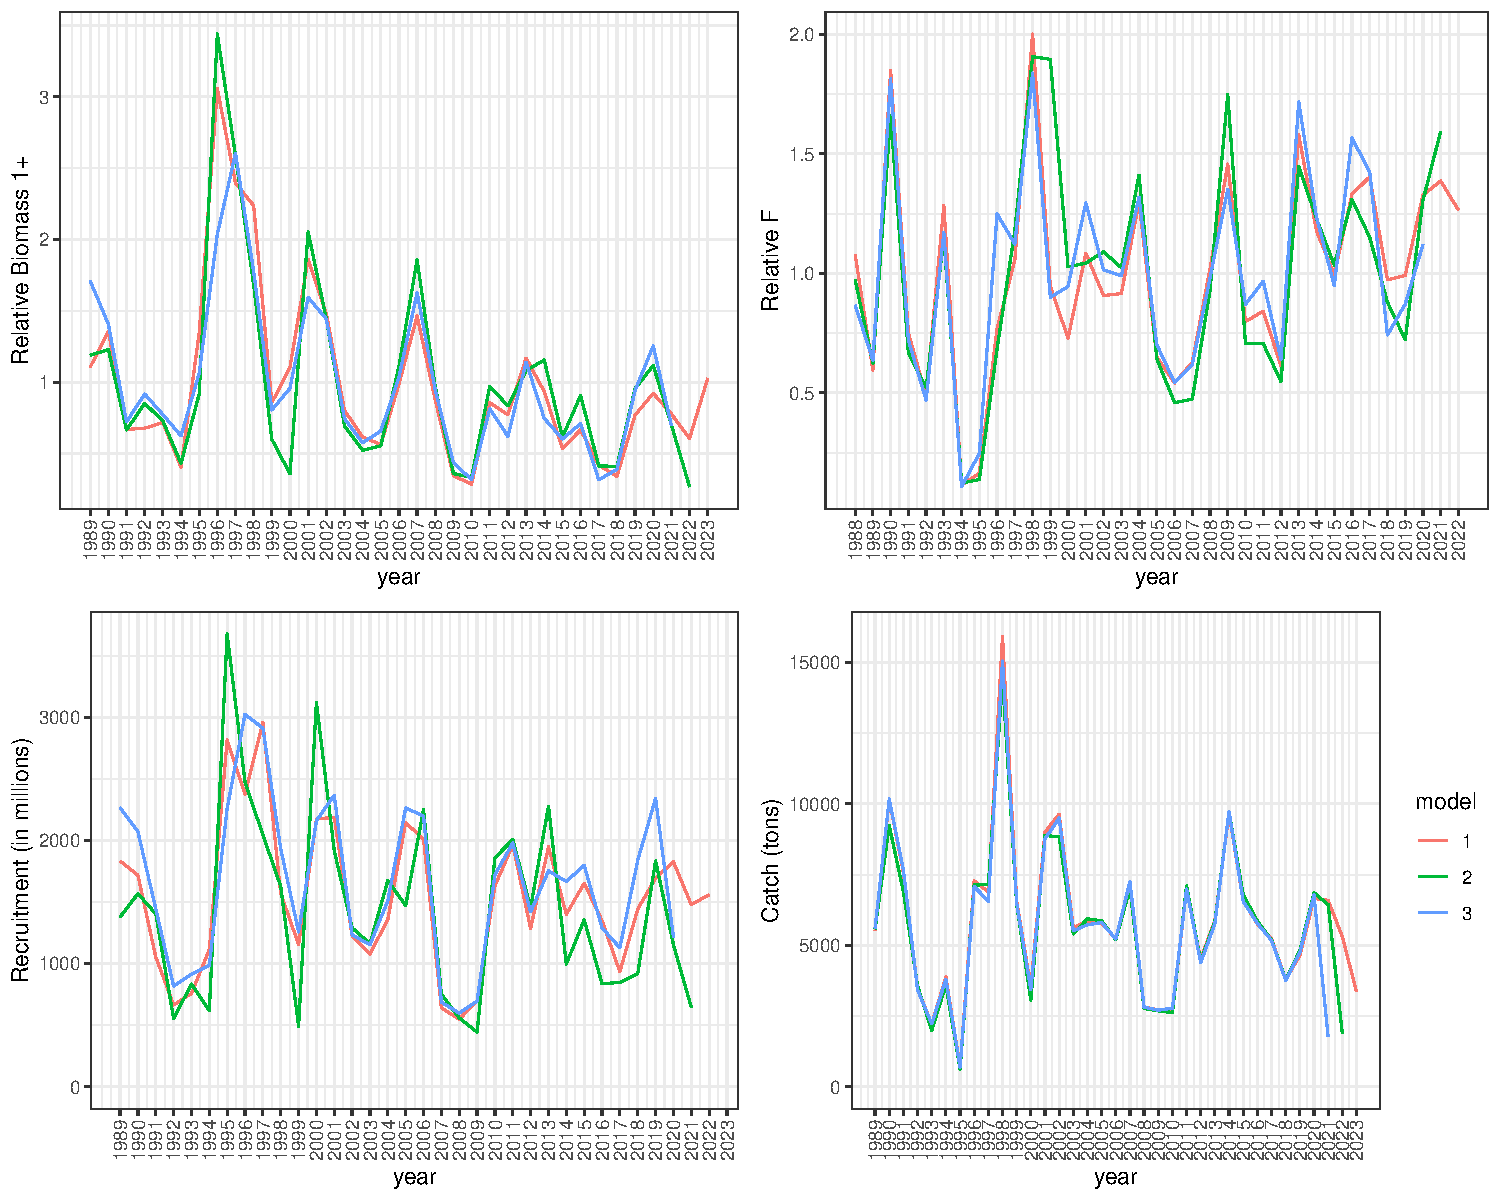
\includegraphics{./ICESplots_modelcomp.pdf}
 % lendist.pdf: 667x841 pixel, 72dpi, 23.53x29.67 cm, bb=0 0 667 841
 \caption{Comparison of estimates from different model implementations.1. Model used last year (pink), 2. Model used last year but including the ECOCADIZ length distribution in 2020 (green), 3. Model described in this document which is the reference for the advice provided in 2022 (blue): Annual model estimates for relative abundance of individuals with more than one year of age, relative fishing mortality, recruitment and catches (in numbers). Measures were summarized at the end of June each year, assuming that a year starts in July and ends in June of the next year. It is also important to remark that the number of iterations for the optimization process in the first model was 2000000, while in the others was just 1000000.}
 \label{modelcomp}
\end{figure}
% \section{Catch advice for July 2018 to June 2019}
% 
% The adviced catches for next year according to the formula decided in WKPELA 2018 (ICES, 2018) would be: $$C_{y+1}=C_{y}\frac{B_{y}}{\overline{B_{y-1}+B_{y-2}}}=\frac{1450}{(4390000+1800)/2}=2520$$, where $B$ represents the estimated abundance by the model as shown in Figure \ref{biomassts} and $C_{y}$ the sum of landings and discards from July of year $y-1$ to June of year $y$.

%3443 capturas algarve y españa 2018 2383.25045 seún Fernando
%para 2017 catches segundo semestre 1224.3816 más discards 122.483

%Para las capturas totales revisar el estesi3_fv_local en GADGET/Assessment/Assessment2018
% TOTALCATCHfv
%       Col1
% 1 3607.638 + discards

%2019 Advice
% \section{Catch advice for July 2019 to June 2020}
% 
% 
% The ratio between the last year biomass estimate and the mean of the two previous years is: $$\frac{B_{y}}{\overline{B_{y-1}+B_{y-2}}}=\frac{3300}{(1450+1800)/2}=3.61$$ for  $B$ representing the estimated abundance by the model as shown in Figure \ref{biomassts}. According to Uriarte et al. (2018) presented in WKLIFEVIII and in accordance with the procedure adopted for Anchovy 9.a. West, it was decided by the group to not apply the rule specified in the Stock annex for 2019 advice, instead, it was decided that adviced catches for the next year would be calculated as follows:  $$C_{y+1}=\hat{C}_{y}\frac{B_{y}}{({B_{y-1}+B_{y-2}})/2}$$ where  $\hat{C}_{y}$ is the value of adviced catches in 2018. Then the adviced catches  (in tonnes) for the next year (July 2019 to June 2020) would be: $$C_{y+1}=4476*\frac{3300}{(1450+1800)/2}  =2520.$$
%2020 advice
% \section{Catch advice for July 2022 to June 2023}
% 
% 
% The ratio between the last year biomass estimate and the mean of the two previous years is: $$\frac{B_{y}}{\overline{B_{y-1}+B_{y-2}}}=\frac{2590}{(3952+3332)/2}=1.486$$ for  $B$ representing the estimated abundance by the model as shown in Figure \ref{biomassts}. According to the report of WKLIFEVX (ICES,2021), if this ratio is above 1.8, the advice would be equal to the latest advice mutiplied by 1.8, and by a biomass safe guard as follows:  $$C_{y+1}=\hat{C}_{y}*\min{1.8,\frac{B_{y}}{({B_{y-1}+B_{y-2}})/2}}*\frac{B_{y}}{I_{trigger}}$$ where  $\hat{C}_{y}$ is the value of adviced catches in the previous year. Then the adviced catches (in tonnes) for the next year (July 2022 to June 2023) would be: $$C_{y+1}=1694*1.49*3.59=2517.3.$$  This procedure modification has been implemented since 2019 and it is not specified in the Stock annex.
%\frac{3950}{(3300+1450)/2}  =2520.$$  This procedure was not specified in the Stock annex for 2020 advice.


%for the next year would be:  $$C_{y+1}=\hat{C}_{y}\frac{B_{y}}{({B_{y-1}+B_{y-2}})/2}$$ where  $\hat{C}_{y}$ is the value of adviced catches in 2019. Then the adviced catches  
 


%=6120$$,  where $\hat{C}_{y}$ is the recommended quota for year $y.$ 

%This ratio is higher than 1.2, then, according to the Stock annex and following the formula decided in WKPELA 2018 (ICES, 2018), the adviced catches  (in tonnes) for the next year would be: $$C_{y+1}=1.2\hat{C}_{y}=2030$$,  where $\hat{C}_{y}$ is the recommended quota for year $y.$ 
%%%%%%%%%For other cases $$C_{y+1}=\hat{C}_{y}\frac{B_{y}}{\overline{B_{y-1}+B_{y-2}}}=1690*\frac{3300}{(1450+1800)/2}=2520$$
%where $B$ represents the estimated abundance by the model as shown in Figure \ref{biomassts}
\section{Reference points}

The methodology applied was the same decided in WKPELA 2018 (page 286 of WKPELA 2018 report (ICES, 2018)) following ICES guidelines for calculation of reference points for category 1 and 2 stocks and the report of the workshop to review the ICES advisory framework for short lived species ICES WKMSYREF5 2017 (ICES, 2017).

According to the above ICES guidelines and the S-R plot characteristics (Figure \ref{SSBt_1rect}), this stock component can be classified as a “stock type 5” (i.e. stocks showing no evidence of impaired recruitment or with no clear relation between stock and recruitment (no apparent $S-R$ signal)). According to this classification, $B_{lim}$ estimation is possible according to the standard method and it is assumed to be equal to $Bloss$ ($B_{lim}=B_{loss}$). For \textbf{2023} the value of $B_{loss}$ for the 9a South anchovy corresponds to the estimated $SSB$ in \textbf{2010} (1226.13 t),  hence $B_{lim}$ is set at 1226.13 t and the relative $B_{lim}$ (divided by the mean value of $B_1+$) results equal to 0.286. Note that due to some inconsistencies in the maturity ogives used in WKPELA2018, age 1+ individuals ($B_1+$) are assumed as mature i.e. $B_1+$ class is equivalent to Stock Spawning Biomass (SSB) (see subsection \ref{ARF} above).
%Note that we are now using 2010 as reference for $Bloss$ instead of 2010 as was done during WKPELA 2018, this is because we found some inconsistencies in the maturity ogives used, and we now assume age 1+ individuals ($B_1+$) as mature (see subsection \ref{ARF} above)
%está en tons 
\begin{figure}[h!]
 \centering
 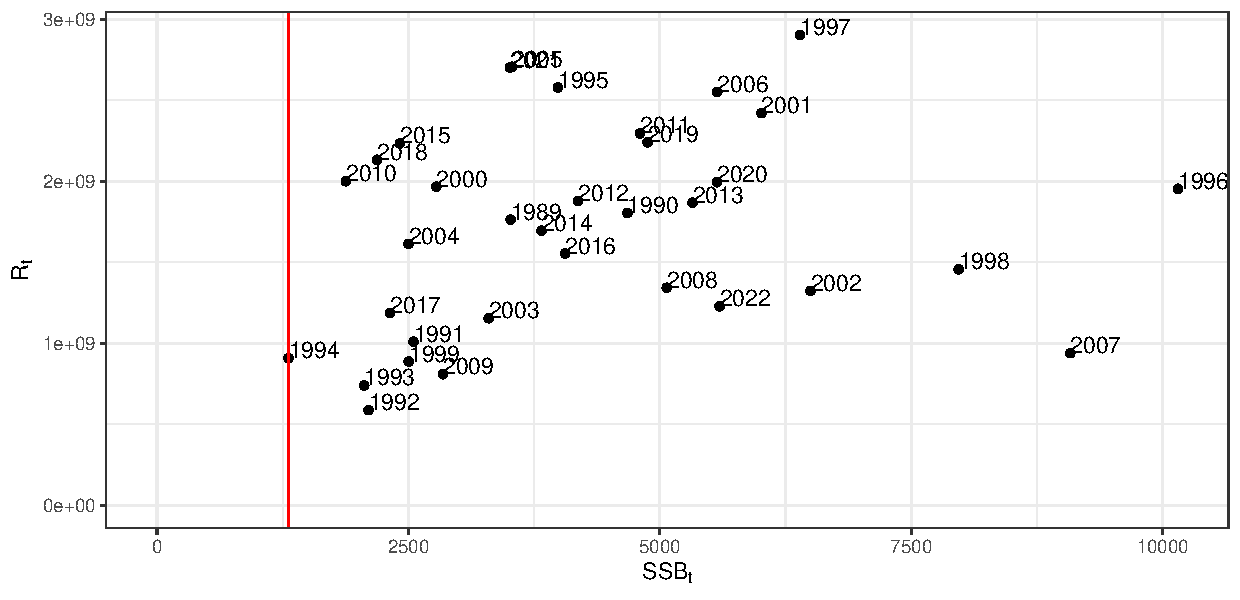
\includegraphics[bb=0 0 595 288]{./SSBt_1rect.pdf}
 % lendist.pdf: 667x841 pixel, 72dpi, 23.53x29.67 cm, bb=0 0 667 841
 \caption{Estimated Stock Spawning biomass ($SSB_{t}$) vs. Recruitment ($R_{t}$), $SSB_{t}$ corresponds to the Stock Spawning Biomass at the end of quarter 2 of year $t$, while $R_{t}$ corresponds to the sum of the recruitment at the beginning of quarters 3,4 and 1 of years $t$ and $t+1,$ respectively.}
 \label{SSBt_1rect}
\end{figure}

ICES recommends to calculate $B_{pa}$ as follows: $$B_{pa} = e^{(1.645\sigma)} B_{lim},$$
where  $\sigma$  is the estimated standard deviation of $ln(SSB)$ in the last year of the assessment, accounting for the uncertainty in $SSB$ for the terminal year.  If $\sigma$ is unknown and for short living species, as it is in our case, it can be assumed that $\sigma = 0.30$ (see page 34 of ICES WKMSYREF5 2017 report (ICES, 2017)), then $B_{pa} = e^{(1.645\sigma)}B_{lim}=1.64B_{lim}$. According to this $B_{pa}$ is set at 2010.8532 t.
% 1.64 can be used as a default for $e^{(1.645\sigma)}$, which corresponds to assume $\sigma = 0.30$ in the (see page 34 of ICES WKMSYREF5 report (ICES, 2017e)) . According to this procedure $Bpa = 1.64Blim$ and $Bpa$ is set at 2.0172 t. 
\section{Catch advice for July 2023 to June 2024}
\subsection{One over two harvest control rule}
The ratio between the last year biomass estimate and the mean of the two previous years is: $$\frac{B_{y}}{\overline{B_{y-1}+B_{y-2}}}=\frac{4402}{(3332+2593)/2}=1.486$$ for  $B$ representing the estimated abundance by the model as shown in Figure \ref{biomassts}. According to the report of WKLIFEVX (ICES,2021), if this ratio is above 1.8, the advice would be equal to the latest advice mutiplied by 1.8, if not,  the latest advice would be multiplied by this ratio. In case the estimated abundance is below a biomass trigger, which in this case is $B_{lim}$, it is also multiplied by a biomass safe guard as follows:  $$C_{y+1}=\hat{C}_{y}*\min\left(1.8,\frac{B_{y}}{(B_{y-1}+B_{y-2})/2}\right)$$ where  $\hat{C}_{y}$ is the value of adviced catches in the previous year. Then the adviced catches (in tonnes) for the next year (July 2023 to June 2024) would be: $$C_{y+1}=1694*1.49=2517.3.$$  This procedure modification has been implemented since this year and it is not specified in the Stock annex.
\subsection{Constant harvest rate rule}
%Sufficient evidence was provided showing that a constant harvest rate of 0.5 is precautionary allowing for a higher catch in the short, medium and long term
According to this rule, adviced catches (in tonnes) for the next year (July 2023 to June 2024) would be the product of the last year biomass estimate and a constant harvest rate. In this case a rate of 0.5 was considered like the most suitable rate for this stock, as follows:
$$C_{y+1}=B_{y}*0.5=4402*0.5=2201.$$
This procedure modification has been implemented since this year and it is not specified in the Stock annex.

%  ICES
% uses Bpa = 1.4 Blim for many of the longer-lived stocks (1.4 is an upward rounding of
% e
% 1.645
% , where =0.2), and it was suggested that a candidate default value for short-lived
% stocks could be σ0.3 (approximately the average of the values in Table 3.2.1) corresponding
% to Bpa = 1.64 Blim




% Figure \ref{SSBt_1rect} presents a comparison between SSB and recruitment, assuming, as mentioned before, that all individuals with age 1 or higher ($B_1+$) are mature. According to that, $Blim$ is equal to 1.23 and relative $Blim$ (divided by the mean value of $B_1+$) equal to 0.286. There are no clear relationship between SSB and recruitment, then according to ICES guidelines for reference points this can be considered as a type 5 case, then $Blim=Bloss$ and $B_{PA}=1.4*Blim=$1.722

%SSB were calculated from estimated total biomass by age using a maturity ogive for the second quarter of each year. Maturity ogive for years 1994,1995 and 1997 weren't available and for those year we used the last year data available. According to that Blim is equal to 1.23 and relative Blim (divided by the man value of ) equal to 0.286
%Parameter estimates and model outputs for age and length distributions of catches and surveys can be found in the Appendix. 
% Frequency distributions  match reasonably well with available data as could be seen in Figures \ref{like}, \ref{agedist} and \ref{lendist}. All the likelihood scores are below 1.5 except for the age distribution of the catches in year 1996, correspondingly there is also a lack of fit in length distribution for that year compared with the other years. According to Figure \ref{ICESplot}, 1996 was the first year with a good recruitment after a 4 years period of bad records. %This remarkable fluctuation could be seen also in the discharges time series (Figure \ref{Displot}), because in 1996 discharges also increased sharply after a severe drought in 1994 and 1995. %A connection between this stock collapse of the fishery in 1995 and the decreases of dam discharges was suggested previously in \citep{Ruiz06}. 











% \begin{figure}[h!]
%  \centering
%  \includegraphics[bb=0 0 595 288]{./discharges88_15Hm3month.pdf}
%  % discharges88_15Hm3month.pdf: 595x288 pixel, 72dpi, 20.99x10.16 cm, bb=0 0 595 288
%  \caption{Quaterly accumulated cubic hectometers that are discharged from Alcalá del Río dam in logarithmic scale.}
%  \label{Displot}
% \end{figure}





%Total mortality $Z$ was approximated using catch at age data with the following equation: $$\log(\frac{C_{1}^{y-1}}{C_{2}^{y}}), y=1990,\dots,2016,$$ where $C_{a}^{y}$ denotes catches in numbers at age $a$ during year $y.$ The results are presented in Figure \ref{Ffromcatches}. Analogously, the same estimation was performed using the age data provided by the ECOCADIZ survey and the results are presented in Figure \ref{Zfromecocadiz}.

%Estimated F for age 1, mean estimated F for Ages 1 and 2 and estimated $Z_{1,2}$ are presented in figure \ref{F1_F12_Z12}.

%High values for $F$ are consistent with the values of $\log(\frac{C_{1}^{y-1}}{C_{2}^{y}}), y=1989,\dots,2015$ where $C_{a}^{y}$ denotes catches in numbers at age $a$ during year $y,$ (see Figure \ref{Ffromcatches}).
% \begin{figure}[h!]
%  \centering
%  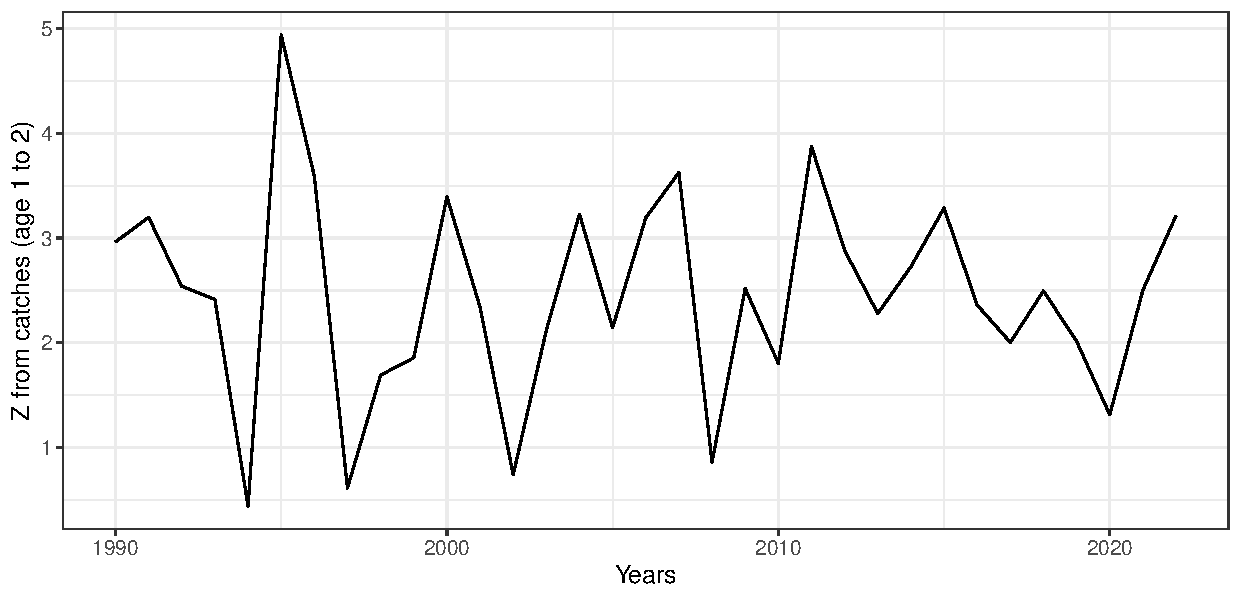
\includegraphics[bb=0 0 595 288]{./Ffromcatches.pdf}
%  \caption{Estimation of Z using information from yearly catch in numbers from individuals of age 1 and 2.}
%  % Ffromcatches.pdf: 307x288 pixel, 72dpi, 10.83x10.16 cm, bb=0 0 307 288
%  \label{Ffromcatches}
% \end{figure}
% 
% \begin{figure}[h!]
%  \centering
%  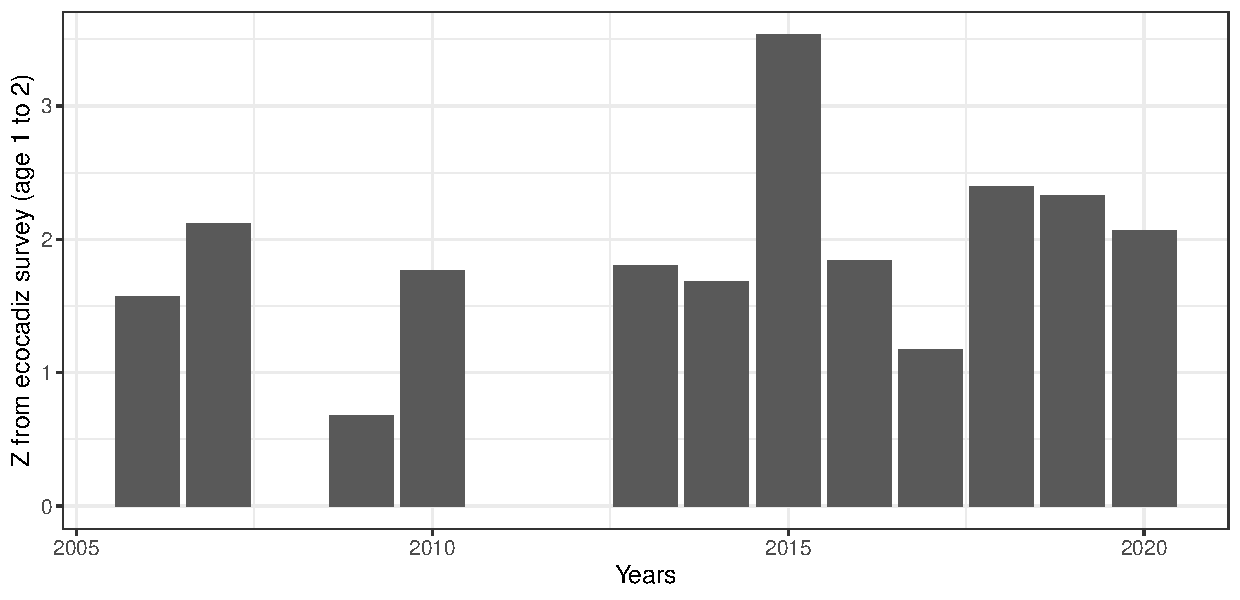
\includegraphics[bb=0 0 595 288]{./Zfromecocadiz.pdf}
%  \caption{Estimation of Z using information from ECOCADIZ age samples from individuals of age 1 and 2.}
%  % Ffromcatches.pdf: 307x288 pixel, 72dpi, 10.83x10.16 cm, bb=0 0 307 288
%  \label{Zfromecocadiz}
% \end{figure}

% \begin{figure}[h!]
%  \centering
%  \includegraphics[bb=0 0 518 432]{./F1_F12_Z12.pdf}
%  \caption{Estimated F for age 1, mean estimated F for Ages 1 and 2 and estimated $Z_{1,2}$ }
%  \label{F1_F12_Z12}
%  % ICESplots.pdf: 523x379 pixel, 72dpi, 18.45x13.37 cm, bb=0 0 523 379
% \end{figure}

% \section{Scenarios to explore}
% \begin{enumerate}
% \item Natural mortality obtained by expert elicitation $M_{0}=1.5, M_{1}=1, M_{2}=1.5, M_{3}=1:$ A bad fitting was obtained showing the sensitivity of the model results to this value. Some variations of this scenario should be explored.
% \item Natural mortality at age estimated by the model
% \item Forecast assuming that the advice is provided:
% \begin{itemize}
% %\item In February of year ‘y+1’ for year ’y+1’ including all the available surveys indices (i.e. for recruitment informed on estimates from ECOCADIZ-RECLUTAS). 
% %\item In June of year ‘y’ for year ‘y+1’ without consider the estimates provided by that survey (i.e. for an assumed scenario of recruitment-uninformed by surveys). 
% \item In June of year ‘y’ for year ‘y+1’ %without consider the estimates provided by that survey and updated in April/May of year 'y+1' by 
% including the PELAGO survey performed in March/April.
% \end{itemize}
% \end{enumerate}
% % The results of the Gadget model presented in the Appendix and in Figure \ref{ICESplot} provides valuable information about the status of the stock,  even not accounting for the influence of environmental covariates on recruitment. From Figure \ref{ICESplot}, it could be claimed that high values of fishing mortality seems to appear as a result of an increase of recruitment (1998, 2002) or as previously stated in \citep{ruiz_biological_2017}  as a result of the fixed quota management where $F$ tends to increase where the recruitment is low (1994, 2004, 2007, 2010) and viceversa (1996, 2011). The model confirms the  BotTop population dynamics regime described before in \citet{ruiz_anchovy_2007} where recruitment is transfered from one year to the next,  together with a very high annual exploitation rate (Between 1 and 4, Figure \ref{ICESplot}, top right panel) that hampers them to survive from one year to the next. In particular, we can see that Gadget explains 1995 collapse as a consequence of a bad recruitment and huge $F$ on the previous year. The trend of abundance estimation is also coherent with the one estimated in \citet{ruiz_bayesian_2009}, but the scale is different, Gadget model yearly abundace estimates are between 0 and 750 millions while the other model quarterly estimates are between 0 and 1500 millions. This difference it is difficult to explain because of the way that fishing mortality ($F$) is accounted in both models, Gadget offers the possibility to estimate $F$ directly in order to make catches forward projections while $F$ is not explicitly defined in the other model, therefore $F$ is easily tracked in Gadget and the estimates are very high while in the other model there is no way to get an output that relates abundance with catches. 
% 







%R
%The final question: How Gadget accounts for the variability added by the environment in stages previous to recruitment?






%This suitability have  used also estimationto be estimated such as 

%Gadget or SS3 are mainly focused in modeling biological processes and their interaction with fishing dynamics 


















%\subsection{Management Strategy Evaluation comparison framework}
%Using the 
% From the recruitment time series modelled with Gadget it is possible to extract a numerical relationship with environmental covariates and make forward projections under different management strategies. This follows from the approach developed by the International Whaling Commission, a management strategy evaluation (MSE) \citep{kirkwood_1997, butterworth and Punt_1999, Kell_2005} that have been extensively used in stock assessment \citep{Kell_2007}.
% 
% 
% 
% 
% The flexibility of this platform allow the analysis of different management scenarios, an and  to provide information on anchovy year classes that constitute the magnitude of the biomass and catches.
% 
% 
% 
% in a robust statistical framework to provide information on year classes.
% 




% dthey have been used separately 
% 
% that can be used together to provide information on year classes
% re isn't an appropriate assessment needs a model that supports the incorporation
% ``the lack of available data on year classes that constitute the bulk of the biomass and catches 
% '' the lack of advice in the last two years \citep{ICES2015} relies on This was due to the lack of 
% available data on year classes that constitute the bulk of the biomass and catches 
% 
% 
% 
% That kind of approach is needed for analysis of anchovy population in the Gulf of Cadiz
% 
% available have estimulate a coherent integration of the information 
% 
% 
% the inclusion 
% of auxiliary  information (i.e. survey indexes, fishing effort, length-weight relationships) in modelling framework have result in
% 
% Estimating likelihood components weights and model parameter optimization as described in \citet{taylor_a_simple_2007} incorporates the information provided by different datasets simultaneously and have been used in multiple fisheries applications
% 
% 
% 
% 
% to estimate parameters have been proved to be useful 
% \section{Front matter}
% 
% The author names and affiliations could be formatted in two ways:
% \begin{enumerate}[(1)]
% \item Group the authors per affiliation.
% \item Use footnotes to indicate the affiliations.
% \end{enumerate}
% See the front matter of this document for examples. You are recommended to conform your choice to the journal you are submitting to.
% 
% \section{Bibliography styles}
% 
% There are various bibliography styles available. You can select the style of your choice in the preamble of this document. These styles are Elsevier styles based on standard styles like Harvard and Vancouver. Please use Bib\TeX\ to generate your bibliography and include DOIs whenever available.
% 
% Here are two sample references: \cite{Feynman1963118,Dirac1953888}.
\newpage

\section{Acknowledgements}
%The research leading to these results has received funding from the European Union Seventh Framework Programme (FP7-KBBE-2013) under the grant agreement 613571/MAREFRAME project and  Margarita M. Rincón was funded by P09-RNM-5358 of the Junta de Andalucía. However, the document does not necessarily reflect EC views and in no way anticipates the Commission's future policy in the area. 
We thank Jamie Lentin from Shuttlethread for the automatization of data input,  Bjarki Elvarsson for having an open repository with very useful Gadget data processing routines and his valuable help, and to the members of WGHANSA group for their guidance and support.

We gratefully thank CESGA (Galician Supercomputing Center) for computational time at the FTII Supercomputer and technical assistance.












%\cleardoublepage

\section{References}

\bibliography{totalfv,Granger,paper1,paper1zotero,RUIZetal,paper2,total}

\appendix
%\numberwithin{equation}{section}
%\numberwithin{figure}{section}
%\numberwithin{table}{section}
% \section{Model description}
% 
% % Here we present the technical details for the implementation of Gadget and simple models using real and simulated data for the Gulf of Cádiz anchovy stock. Real data were extracted from ICES reports as well as from different records that the Instituto Español de Oceanografía has compiled on this stock along the last decades and simulated data were obtained from the minimum realistic model described in \cite{rincon_economic_2016}. 
% 
% The general Gadget model description and all the options available can be found in Gadget manual \citep{begley_gadget_2004} and some specific examples can be found in \citet{taylor_simple_2007} and \citet{elvarsson_bootstrap_2014}. The Gadget model implementation consists in three parts, a simulation of biological dynamics of the population (simulation model), a fitting of the model to observed data using a weighted log-likelihood function (observation model) and the optimization of the parameters using different iterative algorithms.   
% 
% %The simple models chosen are part of a summary of data-limited methods described in \textbf{DLMtool manual} and there is an interactive way to use them available at \url{http://www.datalimitedtoolkit.org/}
% 
% A list of the symbols used and a graph with the Gadget model structure are presented in  Table \ref{Symbols} and Figure \ref{fig:Diagram}, respectively.
% 
% 
% %\subsection{Gadget model using real data}
% 
% 
% 
% %\begin{itemize}
% \subsection{Simulation model}
% %\end{itemize}
% 
% The model consists of one stock component of anchovy (\textit{Engraulis encrasicolus}) in the ICES subdivision, IX.a South-Atlantic Iberian waters, Gulf of Cádiz. Gadget works by keeping track of the number of individuals, $N_{a,l,y,t},$ at age $a = 0, \dots,3$, at length $l = 3,3.5,4,4.5, \dots,22$, at year $y=1988,\dots,2015$, and each year divided into quarters $t =1, \dots, 4.$. The last time step of a year involves increasing the age by one year, except for the last age group, which its age remains unchanged and the age group next to is added to it, like a 'plus group' including all ages from the oldest age onwards \citep{taylor_simple_2007}.
% 
% 
% 
% % specific region defined by $ r $ = IXa (Division 9.a South-Atlantic Iberian waters, Gulf of Cádiz). Gadget works by keeping track of the number of individual and mean weight at age $ a$ = 0.3, at reference weight  , at length $l$ = 3.22 with a step size$ dl $= 0.5 between each length group, with a specified timestep$ t $= 4 for each year ($y$) from 1988 to 2015. The length of the timestep is denoted by $\Delta t$.
% 
% \subsubsection*{Growth}
% The growth function is a simplified version of the Von Bertalanffy growth equation, defined in \citet{begley_gadget_2004} as the LengthVBSimple Growth Function (\textit{lengthvbsimple}).
% Length increase for each length group of the stock is given by the equation below:
% 
% \begin{equation}
% \label{eq:inlen}
% \Delta l =(l_\infty - l)(1-e^{k\Delta t}),
% \end{equation}
% 
% where $\Delta t$ is the length of the timestep, $l_\infty=19 cm$ is the terminal length and $k$ is the growth rate parameter.
% 
% The corresponding increase in weight of the stock is given by:
% 
% \begin{equation}
% \label{eq:inwei}
% \Delta w=a ((l + \Delta l)^b - l^b),
% \end{equation}
% 
% whit $a=2.9e^{-5}$ and  $b=3.3438$ set as fixed and extracted from \citet{millan_reproductive_1999}.
% The growth functions described above calculate the mean growth for the stock within the model. In a second step the growth is translated into a beta-binomial distribution of actual growths around that mean with a parameter $\beta$ to be fitted by the model as described in  \citet{taylor_simple_2007}.% with a parameter $\beta$ to be fitted by the model and defined as in the appendix of \citet{elvarsson_bootstrap_2014}. 
% 
% 
% 
% \subsubsection*{Initial abundance and recruitment}
% 
% Stock population in numbers at the starting point of the simulation is defined as:
% $$N_{a,l,1,1}=10000\nu_{a}q_{a,l}, \quad a=0,\dots,3, l=3,\dots,20$$
% 
% Where $\nu_{a}$ is an age factor to be calculated by the model and $q_{a,l}$ is the proportion at lengthgroup $l$ that is determined by a normal density with a specified mean length and standard deviation for each age group. Mean length at age and standard deviation was extracted from the age-length key calculated with Powell-Weterall methods in \cite{bellido_use_2000}, the standard deviation was chosen as the same for all age groups and equal to the maximum standard deviation (1.5). The mean weight at age for this initial population is calculated by multiplying the reference weight corresponding to the length by a relative condition factor assumed as 1. Reference weight at length $l=3,3.5,\dots,20$ was approximated with an exponential fit ($w=6.74e^{-4}e^{0.23*l}$) using data from length at age (Seasonal Von Bertallanfy growth \cite{bellido_use_2000}) and transforming them to weight with the formula $w=al^{b}, a=0.0038$ and $b=3.19$ for individuals from 1-10 months old and $a=2.9e^{-5}, b=3.3438,$ for individuals older than 10 months \citep{millan_reproductive_1999} . In Gadget files this was specified as a normal condition distribution (\textit{Normalcondfile}).
% % 
% % 
% % The initial conditions section of stock file specifies the stock population at the start of the simu-
% % lation (ie. at the beginning of the first timestep specified in the ”time” file). This includes setting
% % up the population size, the length distribution and the mean weight for each length group. This
% % is done by specifying the minimum and maximum age and length for the stock on this timestep,
% % and either specifying parameters to allow Gadget to create a stock distribution based on a Normal
% % distribution, or the numbers that make up the stock distribution required.
% % The format for the initial conditions section of the stock file is given below:
% % initialconditions
% % minage <minimum age for the initial stock>
% % maxage <maximum age for the initial stock>
% % minlength <minimum length for the initial stock>
% % maxlength <maximum length for the initial stock>
% % dl <step size for the initial length groups>
% % sdev <standard deviation multiplier>
% % <initial stock distribution data>
% % The optional
% % <
% % sdev
% % >
% % value is used to scale the standard deviation of the length of the initial
% % stock. The standard deviation used in calculating the length distribution will be multiplied by
% % this value. If it is not specified, then it is assumed to have a value of 1 (ie, no scaling will take
% % place). The optional
% % <
% % dl
% % >
% % value is used to set the length group divisions for the initial stock
% % population. If this is not specified, then it is assumed that the initial population will have the
% % same value for
% % <
% % dl
% % >
% % as for the stock, as specified in the main stock file.
% % There are three formats for the initial stock distribution data, as given below:
% % Normal Condition - use a Normal function to generate the length distribution, with a relative
% % condition factor to assign a mean weight to the initial population
% % 
% % 
% % 
% % A Normal function is applied to generate the length distribution, with a relative condition factor to assign to the mean weight of the initial population. The first step will be the construction of a population of 10,000 fish for each age group that is then multiplied by an age weighting factor and an area weighting factor to get to the initial population used in the model. Afetr that, a Normal distribution is applied to a specified mean length with a specified standard deviation in order to generate length groups for these age groups. The mean weight for this initial population is calculated by multiplying the reference weight by a relative conditioning factor \cite{bellido2000use}.
% 
% 
% Similarly to the process to calculate the initial abundance described above, the recruitment specifies how the stock will be renewed. Recruits for $t=3,4$ and $t=1,2$ enter to the age 0 and age 1 population, respectively, as follows: $$N_{0,l,y,t}=p_{l,t}R_{y,t}, \quad t=3,4, l=3, \dots,15,$$ and $$N_{1,l,y,t}=p_{l,t}R_{y,t}, \quad t=1,2, l=3, \dots,15,$$ where $R_{y,t}$ represents recruitment at year $y$ and quarter $t,$ and $p_{l,t}$ the proportion in lengthgroup $l$ that is recruited at quarter $t$ which is sampled from a normal density with mean ($\mu$) and standard deviation ($\sigma_t$) calculated by the model. The mean weight for these recruits is calculated by multiplying the reference weight corresponding to the length by a relative condition factor assumed as 1. Reference weight at age was the same used to calculate the initial population mean weight at age explained above.  In gadget files this was specified also as a normal condition distribution (\textit{Normalcondfile}).
% 
% 
% % \subsubsection*{Natural mortality}
% % 
% % In the simulation the natural mortality is simply modelled as the proportion of the stock that is removed due to these additional causes from each age group, on each timestep, as shown in equation below:
% % 
% % \begin{equation}
% % \label{eq:natmor}
% % N_a = e^{- M_a \Delta t}
% % \end{equation}
% % 
% % The natural mortality parameters $M_a$  are specified as a vector, with one parameter per age group.
% 
% \subsubsection*{Fleet operations}
% 
% In the model the fleets act as predators.  There are three fleets inside the model: two for acoustic surveys (ECOCADIZ and PELAGO) and one for commercial landings (purse-seine fleet). Acoustic surveys fleets are assumed to remove 1 $Kg$ in each of the quarters when the surveys take place. Commercial fleet is assumed to remove a number of individuals each quarter based on reported total landings (extracted from ICES reports). Catches are simulated based on these data available for the fleets and a length based suitability function%. Then,
% %landings in number. A suitability function is also to be defined for the predation of the stocks in the model.
%  that splits the total amount landed by surveys (in biomass, totalfleet)  and the commercial fleet (in numbers, numberfleet) between the length groups, according to equations \ref{eq:totfleet} and \ref{eq:nfleet}  respectively, as follows:
% 
% 
% \begin{equation}
% \label{eq:totfleet}
% C_{l,y,t}  =  \frac{E_{y,t} S_{l,T} N_{l,y,t} W_{l}}{\sum\limits_l S_{l,T} N_{l,y,t} W_{l} },
% \end{equation}
% and
% \begin{equation}
% \label{eq:nfleet}
% C_{l,y,t}  =  \frac{E_{y,t} S_{l,T} N_{l,y,t} }{\sum\limits_l S_{l,T} N_{l,y,t} }, 
% %C_{ns(l)} = \frac{E_b S_{s(l)} N_{sl}}{\sum\limits_s \sum\limits_l S_{s(l)} N_{sl} }
% \end{equation}
% 
% where $E_{y,t}$ represents biomass landed (in $Kg$) at year $y$ and quarter $t$ in equation \ref{eq:totfleet} and numbers landed in equation \ref{eq:nfleet}, $W_l$ corresponds to weight at length and $S_{l,T}$ represents the suitability function that determines the proportion of prey of length $l$ that the fleet is willing to consume during period $T, T=1,2,$ where $T=1$ corresponds to the period 1988-2000 and $T=2$ to 2001-2015.
% 
% %how the fleets act on the stock and it is defined as:
% For this model the suitability function is specified in Gadget manual as an ExponentialL50 function (\textit{expsuitfuncl50}), and it is defined as follows:
% 
% \begin{equation}
% \label{eq:sut}
% S_{l,T}  =  \frac{1}{1+e^{-4 \alpha_{T} (l-l_{50,T})}} 
% \end{equation}
% 
% where $l_{50,T}$ is the length of the prey with a 50\% probability of predation during period T and $\alpha_{T}$ a parameter related to the shape of the function, both parameters are estimated from the data within the Gadget model. The whole model time period (1988-2015) has been splited into two different periods for suitability parameters because of changes in size regulation for the fishery around 1995 that become effective around 2001. 
% 
% %Parameters $\alpha$ and $l_{50}  Parameters 
% 
% 
% % in th and $S_{s(l)}$ is the suitability function of length group that determines how the predators act on the preys, defined according to the equation below:
% % 
% % \begin{equation}
% % \label{eq:sut}
% % S_{s(l)} = \frac{1}{1+e^{-4 \alpha (l-l_{50})}}
% % \end{equation}
% % 
% % This is a suitability function that has no dependence on the length of the predator, and a logarithmic dependence on the length of the prey.
% % 
% % In a different manner to the equation (4) above the catches for commercial fleets are simulated based on reported total landings by number and for length group l they are calculated as:
% % 
% % 
% % 
% % where E is the number caught by the fleet and S is the suitability function of length group defined in the equation (5).
% 
% %\begin{itemize}
% \subsection{Observation model}
% %\end{itemize}
% 
% Data are assimilated by Gadget using a weighted log-likelihood function.  The model uses as likelihood components three biomass survey indices (ECOCADIZ, PELAGO and SAR), age - length distributions from two surveys (ECOCADIZ and PELAGO) and one commercial fleet (purse-seine) and mean length at age distribution from that commercial fleet (see Table \ref{likedesc} for an overview of the likelihood data used in the model). 
% 
% \subsubsection*{Biomass Survey indices}
% 
% The survey indices are defined as the total biomass of fish caught in a survey. The survey index is compared to the modelled abundance using a log linear regression with slope  equal to 1  (\textit{fixedslopeloglinearfit}), as follows:
% 
% \begin{equation}
% \label{eq:surind}
% \ell=\sum\limits_t (\log(I_{y,t}) - (\alpha+\log(N_{y,t}))^2
% \end{equation}
% 
% where $ I_{y,t}$ is the observed survey index at year $y$ and quarter $t$ and $ N_{y,t}$ is the corresponding population abundance calculated within the model. Note that the intercept of the log-linear regression, $\alpha=\log (q),$ with $q$ as the catchability of the fleet (i.e $I_{y,t}=q N_{y,t}$).
% 
% \subsubsection*{Catch distribution}
% 
% Age-length distributions are compared using $l$ lengthgroup at age $a$ and time-step $y,t$ for both, commercial and survey fleets with a sum of squares likelihood function (\textit{sumofsquares}):
% 
% \begin{equation}
% \label{eq:catdis}
% \ell= \sum\limits_y \sum\limits_t \sum\limits_l (P_{a,l,y,t} - \pi_{a,l,y,t})^2
% \end{equation}
% 
% where $P_{a,l,t,y}$ is the proportion of the data sample for that time/age/length combination, while $\pi_{a,l,t,y}$ is the proportion of the model sample for the same combination, as follows:
% \begin{equation}
% P_{a,l,t,y}=\frac{O_{a,l,y,t}}{\sum\limits_a \sum\limits_l  O_{a,l,y,t} }
% \end{equation}
% and
% \begin{equation}
% \pi_{a,l,t,y}=\frac{ N_{a,l,y,t}}{\sum\limits_a \sum\limits_l  N_{a,l,y,t} },
% \end{equation}
% where  $O_{a,l,y,t}$ corresponds to observed data. 
% 
% 
% When only length or age distribution is available. It is compared using equation \ref{eq:catdis} described above but considering all ages or all lengths, respectively.
% 
% 
% \subsubsection*{Catch statistic}
% 
% Mean length at age for commercial fleets are compared using an unweighted sum of squares of mean length likelihood function (\textit{lengthnostddev}):
% 
% \begin{equation}
% \label{eq:catstat}
% \ell=\sum\limits_y \sum\limits_t \sum\limits_a ((x_{a,y,t} - \mu_{a,y,t})^2 N_{a,y,t})
% \end{equation}
% 
% where $x_{a,y,t}$ is the sample mean weight from the data for the timestep/age combination, $\mu_{a,y,t}$ is the mean lenght at age calculated from the model for the same combination and $N_{a,y,t}$ is the number of individuals for the same combination.
% 
% \subsubsection*{Understocking}
% If the total consumption of fish by all the predators (fleets in this case) amounts to more than the biomass of prey available, then the model runs into "understocking". In this case, the consumption by the predators is adjusted so that no more than 95\% of the available prey biomass is consumed, and a penalty, given by the equation \ref{eq:under}  below, is applied to the likelihood score obtained from the simulation (Stefansson 2005 sec 4.1).
% 
% \begin{equation}
% \label{eq:under}
% \ell=\sum\limits_t  U_{t}^{2}
% \end{equation}
% 
% where $U_{t}$ is the understocking that has occurred in the model for that timestep.
% 
% \subsubsection*{Penalties}
% The BoundLikelihood likelihood component is used to give a penalty weight to parameters that have moved beyond the bounds in the optimisation process. This component does specify the penalty that is to be applied when these bounds are exceeded.
% 
% 
% \begin{equation*}
% \ell_i= \begin {cases}
% lw_i(val_i - lb_i)^{2} &\text{if $val_i < lb_i$} \\
% uw_i(val_i - ub_i)^{2} & \text{if $val_i > ub_i$} \\
% 0 & otherwise
% \end{cases}
% \end{equation*}
% 
% Where $lw_i=10000$ and $uw_i=10000$ are the weights applied when the parameter exceeds the lower and upper bounds, respectively, $val_i$ is the value of the parameter and, $lb_i$ and $ub_{i}$ are the lower and upper bounds defined for the parameter.
% 


 

% \begin{table}[h]
% \centering
% \small\small
% \label{Symbols}
% \begin{tabular}{l l l}
% \textbf{Index}   \\
% \it t & Timestep, $ t $= 1,...,4 \\
% \it r & Area, $ IX_a$ South division \\
% \it a & Age, $ a $ = 0,...,3  \\
% \it l & Length, $ l $ = 3,...,22 with step size for lenght group $ dl $ = 0.5                    \\                              \it    s       &    Anchovy Stock                              \\
%  \it b       &    Biomass                                    \\
% \it n       &    Number                                     \\
% \textbf{Parameters}    \\
% $m_a$  &   Natural mortality parameters    \\
% $\alpha$ &   Upper asymptote          \\
% $\beta  $ &     Growth range                            \\
% \it k       &   Annual growth rate               \\
% $ l_\infty$  &   Terminal length                \\
% $l_{50} $ & Length of the prey with a 50 \% probability of predation \\
% $P_i$    &  Power coefficient (which should be 2 for sum of squares fit)                \\
% $lw_i$ and $uw_i$   &  Weight applied when the parameter exceeds the lower and upper bound            \\
% $lb_i$ and $ ub_i $  &  Lower and upper bound            \\
% $val_i $    &   Value of the parameter           \\
% \textbf{Data}        \\
% \it $E_n$   & Number catch by commercial fleet \\
% \it $E_b  $ & Biomass catch by survey fleet \\
% $N_{sl}$    &     Number of stock in the length group \\
% $W_{sl}$   &     Mean weight of the stock in the length group \\
% $P_{tral}$  &    Proportion of the data sample for that time/area/age/length combination      \\
% $I_t$  &  Observed survey index \\
% $x_{tra}$  &  Sample mean length from the data   \\
% \textbf{Others}   &  \\  
% $C_{ns(l)}$ &    Number fleet, catches number at stock $ s $ and at lengthgroup $ l $ of commercial fleet          \\
% $C_{bs(l)} $&    Total fleet, catches biomass at stock $ s $ and at lengthgroup $ l $ of survey fleet         \\
% $S_{s(l)}$  &    Suitability of lengthgroup $ l $           \\
% R  &    Recruitment     \\
% $w_l$ & Reference weight of the stock for various length groups \\
% $N_a $  &    Natural mortality \\
% $\Delta L $ &   Increase in the length for each length group   \\
% $\Delta W$  &   Increase in weight  \\
% $U_{trp}$  & Understocking that has occurred in the model  \\
% $\pi_{tral}$ &      Proportion of the model sample for that time/area/age/length combination   \\
% $\mu_{tra}$  & Mean length calculated from model \\
% $N_{tra}$  &  Sample size \\
% $N_t $ &  Survey index calculated in the Gadget  \\
% 
% \end{tabular}
% \caption{List of Symbols used in model specification}
% \end{table}

% \begin{figure}[h]
% \centering
% \includegraphics[page=1,angle=90,width=0.95\textwidth]{Gadget_dia.pdf} 
% \caption{Graph Gadget model}
% \label{fig:Diagram}
% \end{figure}


% \begin{table}[h]
% \centering
% \small\small
% \label{likedesc}
% \begin{tabular}{l| l l l}
% Data source & type & Timespan & Likelihood function  \\
% \hline
% Commercial landings & Length distribution & All quarters, 1988-2015 & See eq. \ref{eq:catdis}\\
% & Age distribution & All quarters, 1988-2015 &  See eq. \ref{eq:catdis}\\
% & Mean length at age of landings & All quarters, 1988-2015 & See eq. \ref{eq:catstat} \\
% ECOCADIZ survey & Biomass survey indexes & Second quarter 2004, 2006 & see eq. \ref{eq:surind}\\
% & & third quarter 2007, 2009, 2010, 2013 and 2014 & \\
% & Age-length distribution & Second quarter 2004, 2006 & see eq. \ref{eq:catdis}\\
% & & third quarter 2007, 2009, 2010, 2013 and 2014 & \\
% PELAGO survey & Biomass survey indexes & First quarter 1999, 2001-2003 &  see eq. \ref{eq:surind}\\
% & & second quarter 2005-2010 and 2014 & \\
% & Age-length distribution &  First quarter 1999, 2001-2003 &  see eq. \ref{eq:catdis}\\
% & & second quarter 2005-2010, 2013 and 2014 & \\
% SAR survey  & Biomass survey indexes & Last quarter 1998, 2000,2001, 2007 and 2012 &  see eq. \ref{eq:surind}\\
% \hline
% \end{tabular}
% \caption{Overview of the likelihood data used in the model}
% \end{table}

% \subsubsection*{Iterative  re-weighting}
% 
% The total objective function is a weighted sum of all likelihoods components. The weight for each component is determined with an iterative process following the approach presented in \citet{taylor_simple_2007} and in the apppendix of \citet{elvarsson_bootstrap_2014} based on the iterative reweighting scheme of \citet{stefansson_comparing_1998} and \citet{stefansson_issues_2003}, which is summarized as follows:
% 
% Let $\mathbf{w_{r}}$ be a vector of length $L$ with the weights of the likelihood components (excluding understocking and penalties) for the run $r,$ and $SS_{i,r}, i=1,\dots,L,$ the likelihood score of component $i$ after run $r.$  First, a Gadget optimization run is performed  to get a likelihood score ($SS_{i,1}$) for each likelihood component assuming that all components have a weight equal to one, i.e., $\mathbf{w_{1}}=(1,1,\dots, 1).$  Then, a separated optimization run for each of the components ($L$ optimization runs) is performed  using  the following weight vectors:
% $$\mathbf{w_{i+1}}=(1/SS_{1,1},\dots, (1/SS_{i,1})*10000,1/SS_{i+1,1},\dots,1/SS_{L,1}), i=1, \dots,L.$$
% Resulting likelihood scores $SS_{i,i+1}$ are then used to calculate the residual variance, $\hat{\sigma}_{i}^{2}=SS_{i,i+1}/df^*$ for each component, that is used to define the final weight vector as $$\mathbf{w}=(1/\hat{\sigma}_{1}^{2},\dots, 1/\hat{\sigma}_{L}^{2}).$$
% 
% Degrees of freedom $df^*$ is approximated by the number of non-zero data points in the observed data for each component.
% 

%inverse of SS for each component as weight and then this run is compared with those from the iterative reweighting scheme of \citet{stefansson_comparing_1998,stefansson_issues_2003}. The general idea is to use the inverse variance of the residuals of the former comparison are assigned as weights .
% Modeling details can be found in the appendix.
%
%
%
%
%
% Sea surface temperature (SST), discharges from the Alcal{\'a} del R{\'i}o reservoir and wind from 1996 to 2004, were obtained as follows: SST was extracted from  the Advanced Very High Resolution Radiometer (AVHRR) sensor data. The nighttime AVHRR PATHFINDER SST v5 weekly means with $4 \times 4 \quad km^{2}$ pixel resolution were taken from NASA PO.DAAC website (http://podaac.jpl.nasa.gov/). The  region of interest was acquired from the global image and arithmetic means were calculated based on all pixels within this region. Discharges  were provided by Confederaci{\'o}n Hidrogr{\'a}fica del Guadalquivir. They correspond to the monthly accumulated cubic hectometers that are discharged from the reservoir each month. Wind data are the weekly accumulated time (in days) that easterlies faster than $30 \quad km h^{-1}$ have been recorded in the meteorological station of C{\'a}diz.
%
%
% obtained from public databases
% Historical records of environmental covariates
%
% Individuals that have survived for five months, % $B_{t,s}(5),$
% are  considered  recruits and  are included in the stock population size owing to their availability to the fishery. The fishery closes from November to February approximately each year to allow growth of individuals spawned from May to September \citep{ices2012}.
%
%
%
%
%
% Gadget implementation
% combines a large pool of data from diverse sources to diagnose the stock dynamics.
%
%
%
% In this section we give a general description of the %data,
% models and data used, as well as the
%
%
% models, and indicators upon which we \textit{have} focused. We have chosen %two
% \textit{some models used for the assessment of data poor stocks}
% %models, a data limited methods (DLMtool)
% and a Gadget model.
%
% % DLMtool is a free R software package for management strategy evaluation and implementation of data-limited fishery stock assessment methods. The simple models used in this case study are models previously developed for data-limited approaches. A user-friendly tool, the Data-Limited Methods Toolkit \url{http://www.datalimitedtoolkit.org}, recognizes which of the acceptable methods can be applied to the data for the stock and then implement them, eventually, estimating indicators.
%
% Gadget is a parametric and deterministic \textit{age-length-structured} forward population dynamics simulation model\textit{. It} %that
% estimates population dynamics parameters based on fisheries data %and allows the coupling of a model with
% \textit{allowing the use of} an extensive set of data comparison and optimisation routines. Gadget works by running \textit{several times} an internal model based on many parameters, and then comparing the data from the output of this model to observed data to get
% \textit{the best}
% %a
% goodness-of-fit
% %likelihood score
% %The parameters can then be adjusted, and the model re-run, until an optimum is found, which corresponds to the model with the lowest likelihood score. Each stock is de???ned by specifying the length groups, age groups, and length-weight relationship to be used, along with the functions required to simulate the biological processes that affect the stock
% \cite{begley&howell2005}. %Gadget models have been developed using a specialised R-package, Rgadget.
% The standard model and the detail of the general model are described in \cite{begley2004gadget} and in \cite{taylor2007simple}.
%
% DLMtool is a free R software package for management strategy evaluation and implementation of data-limited fishery stock assessment methods. The simple models used in this case study are models previously developed for data-limited approaches. A user-friendly tool, the Data-Limited Methods Toolkit \url{http://www.datalimitedtoolkit.org}, recognizes which of the acceptable methods can be applied to the data for the stock and then implement them, eventually, estimating indicators.

%The comparisons across models must be based on value resulting from the estimates, which are called indicators. The indicators were calculated based on the output produced by the models. All the models estimate indicators with different approach to calculate the TAC value. The value obtained were then used to perform model comparisons. We focus upon two comparisons, one using real data and one using a MSE approach with simulated data.
% \subsection{Fit to data}
% 
% Model outputs for length and age distributions are presented in Figures \ref{agedist} and \ref{lendist}.
% 
% 
% \begin{figure}
% \centering
%  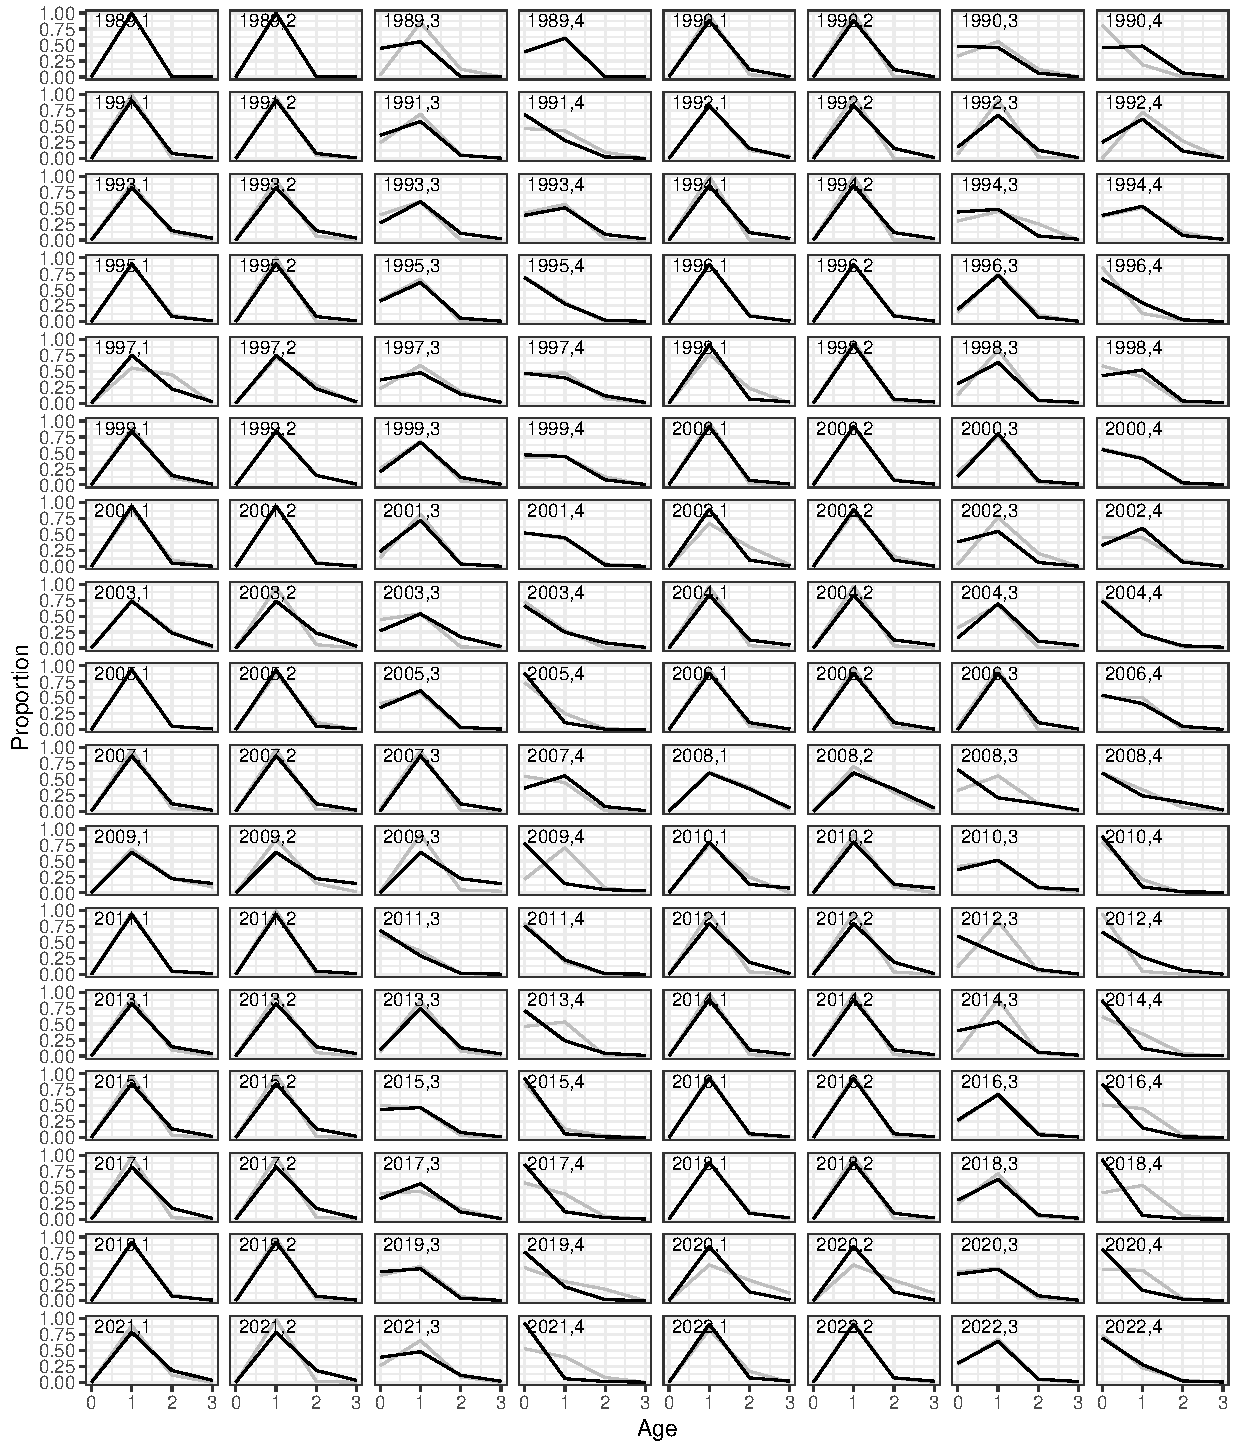
\includegraphics[bb=0 0 523 697]{./agedist.pdf}
%  % agedist.pdf: 667x841 pixel, 72dpi, 23.53x29.67 cm, bb=0 0 667 841
%  \caption{ Comparison between observed and estimated catches age distribution. Black lines represent observed data while gray lines represent estimated data.}
%  \label{agedist}
% \end{figure}
% \begin{figure}[h!]
%  \centering
%  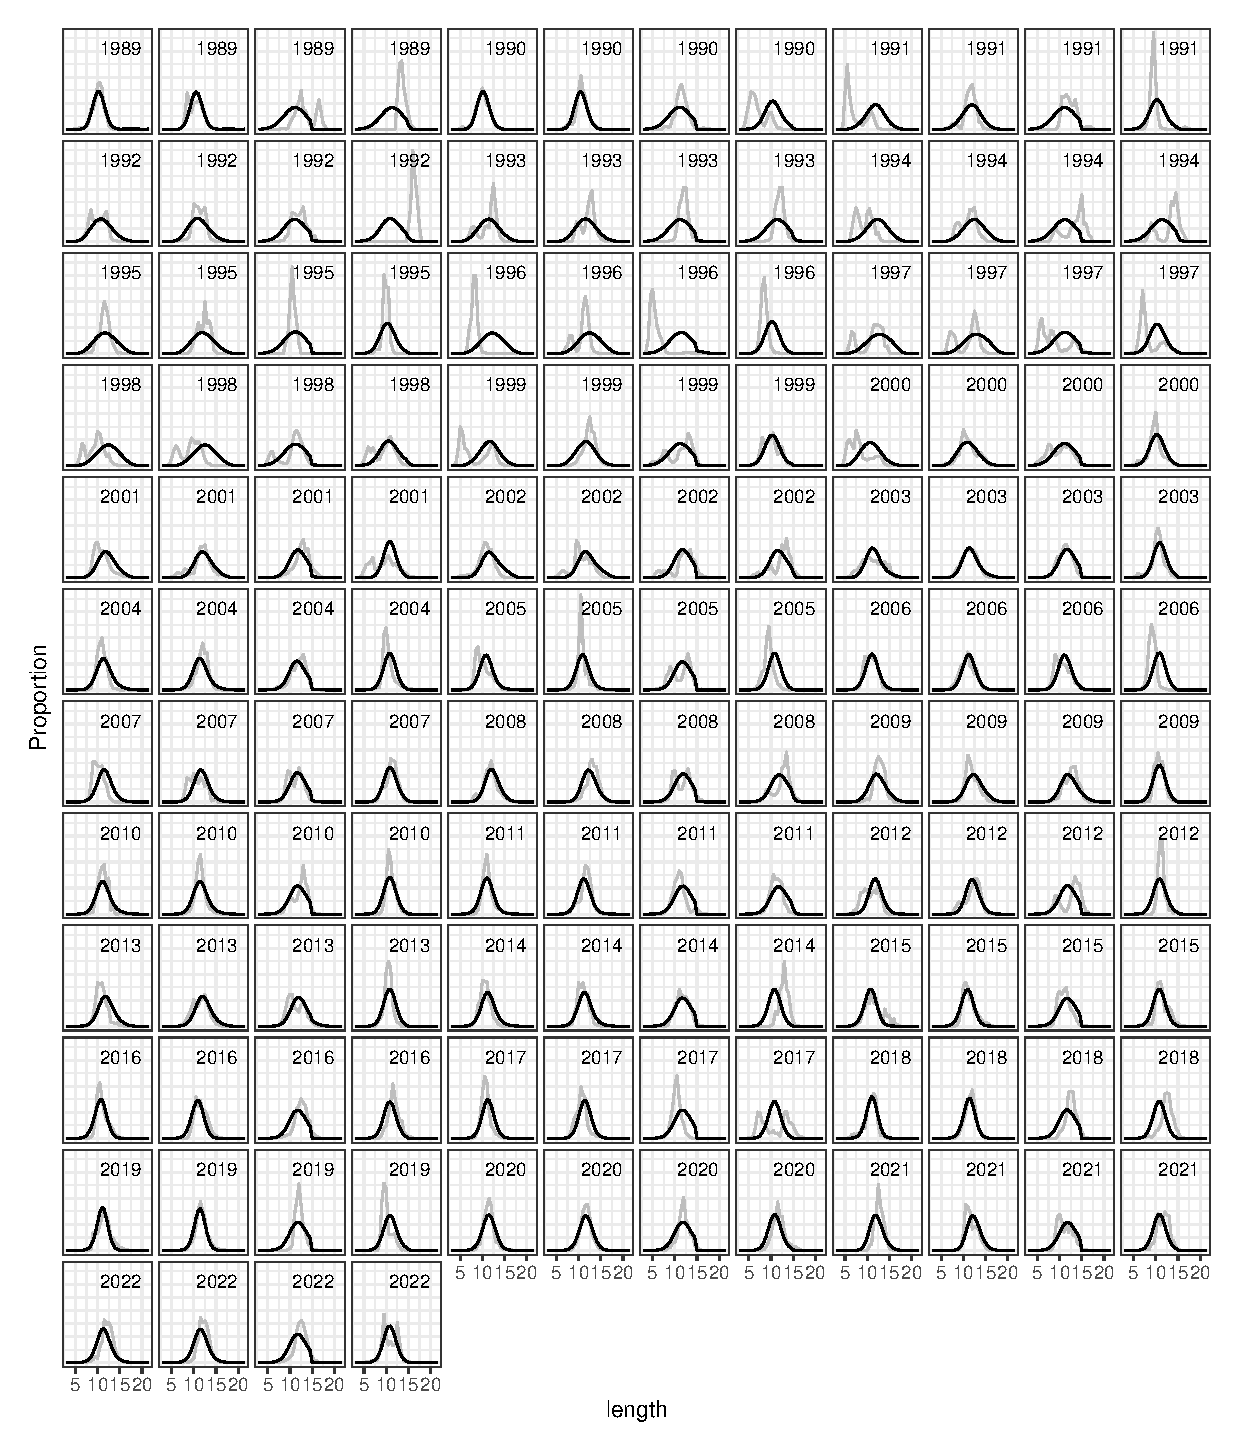
\includegraphics[bb=0 0 523 697]{./lendist.pdf}
%  % lendist.pdf: 667x841 pixel, 72dpi, 23.53x29.67 cm, bb=0 0 667 841
%  \caption{ Comparison between observed and estimated catches length distribution. Black lines represent observed data while gray lines represent estimated data}
%  \label{lendist}
% \end{figure}

% \subsection*{Real data}
% 
% In the comparisons using real data the information were extracted from ICES reports (public) and from IEO datasets (non public).
% 
% The following datasets are used in Gadget for likelihood components. Gadget classify this information as different types of components, time period and component are specified in parenthesis:
% 
% \begin{itemize}
% \item Length distribution of landings (1988-2015, catchdistribution)
% \item Age distribution of landings (1988-2015, catchdistribution)
% \item Landings mean length at age of landings (1988-2015, catchstatistics)
% \item Biomass survey indexes from ECOCADIZ survey. (Second quarter 2004, 2006; third quarter 2007, 2009, 2010, 2013 and 2014, surveyindexes)
% \item Age and length distribution of survey ECOCADIZ (Second quarter 2004, 2006; third quarter 2007, 2009,2010, 2013 and 2014, catchdistribution)
% \item Biomass survey indexes from PELAGO survey. (First quarter 1999, 2001-2003, second quarter 2005-2010 and 2014, surveyindexes)
% \item Age and length distribution of survey PELAGO (First quarter 1999, 2001-2003, second quarter 2005-2010, 2013 and 2014, catchdistribution)
% \item Biomass survey indexes from SAR survey. (Last quarter 1998, 2000,2001, 2007 and 2012, surveyindexes)
% \end{itemize}
% 2010/477/EU: Commission Decision of 1 September 2010 on criteria and methodological standards on good environmental status of marine waters (notified under document C(2010) 5956) Text with EEA relevance


 %European
% Commission
% (2008a).
% Communication
% from
% the
% Commission
% to
% the
% Council
% and
% the
% European
% Parliament:
% The
% role
% of
% the
% CFP
% in
% implementing
% an
% ecosystem
% approach
% to
% marine
% management.
% COM(2008)
% 187,
% 11.4.2008

\end{document}
